
\documentclass[11pt]{jsreport}
%\documentclass{jsreport}
\usepackage[utf8]{inputenc}
\usepackage[dvipdfmx,colorlinks=true, bookmarks=true,bookmarksnumbered=true, bookmarkstype=toc, linkcolor=blue,urlcolor=blue, citecolor=blue]{hyperref}
\usepackage{pxjahyper}
\usepackage[dvipdfmx]{graphicx}
\usepackage[dvipdfmx]{color}
\usepackage{multirow}
\usepackage{here}
\usepackage{amsmath}
\usepackage{float}
\usepackage{url}
\usepackage{setspace}
\usepackage{caption}
\usepackage{subcaption}
\usepackage{lineno}




% ユーザー変数
\newcommand{\myname}{中村 竜也}
\newcommand{\studentid}{211S114S}
\newcommand{\submitdate}{令和5年2月3日}
\newcommand{\papertitle}{LHC-ATLAS実験Run-3における\\初段ミューオントリガーの機械学習を用いた最適化}

\newcommand{\ctext}[1]{\raise0.2ex\hbox{\textcircled{\scriptsize{#1}}}} %丸文字を\ctext{}で入力できるようにする
\newcommand{\unit}[1]{\ \mathrm{#1}} %\unit{}で単位を入力できるようにする。
\newcommand{\siki}[1]{式(\ref{#1})} %式の参照を楽に
\newcommand{\zu}[1]{図\ref{#1}} %図の参照を楽に
\newcommand{\hyou}[1]{表\ref{#1}} %表の参照を楽に
\newcommand{\setu}[1]{\ref{#1}節}
\newcommand{\syou}[1]{第\ref{#1}章}
\newcommand{\pt}{p_\mathrm{T}}

\makeatletter %数式,図,表番号に章番号も含む
\@addtoreset{equation}{chapter}
\def\theequation{\thechapter.\arabic{equation}}
\@addtoreset{figure}{chapter}
\def\thefigure{\thechapter.\arabic{figure}}
\@addtoreset{table}{chapter}
\def\thetable{\thechapter.\arabic{table}}
\makeatother




\begin{document}
\addtocounter{page}{-3}
\thispagestyle{empty}

\vspace*{1.5cm}

\newcommand{\kintou}[2]{%
  \leavevmode
  \hbox to #1{%
    \kanjiskip=0pt plus 1fill minus 1fill
    \xkanjiskip=\kanjiskip
    #2}}

\begin{center}
  \begin{huge}
    修  士  学  位  論  文
  \end{huge}

  \vspace{2cm}

  \begin{huge}
    \begin{spacing}{1.1}
      \fontsize{18.4pt}{20pt}\selectfont
        LHC-ATLAS実験Run-3における\\新ミューオントリガーアルゴリズムの動作検証と改良
    \end{spacing}
  \end{huge}
  
  \vspace{3cm}

  \begin{LARGE}
    \begin{spacing}{1.1}
        \flushright \submitdate\\
        \vspace{1cm}
            \begin{center}
                \begin{tabular}{p{6.5em}p{6.5em}}
                    \kintou{4em}{専攻名}   & 物理学専攻 \\
                    \kintou{4em}{学籍番号} & 220s126s   \\
                    \kintou{4em}{氏名}     & 山下 智愛 \\
                \end{tabular}                
            \end{center}
    \end{spacing}
  \end{LARGE}

  \vspace{4.0cm}

  \begin{LARGE}
    \fontsize{17pt}{20pt}\selectfont
    神戸大学大学院理学研究科博士課程前期課程
  \end{LARGE}
\end{center}
\begin{comment}

\newpage
~
\thispagestyle{empty}
\newpage
\thispagestyle{empty}
\newpage
%\linenumbers

%----abstract----
\begin{center}
    \begin{large}
        令和5年度~修士論文発表会概要 
    \end{large}
\end{center}

\begin{center}
  \begin{Large}
     LHC-ATLAS実験Run-3における\\新ミューオントリガーアルゴリズムの動作検証と改良
  \end{Large}
\end{center}

\begin{flushright}
    粒子物理学研究室~220s126s~山下智愛 \\
    指導教員~山\ajTatsuSaki 祐司
\end{flushright}

\vspace{10pt}

Large~Hadron~Collider~(LHC)は欧州原子核機構~(CERN)によってスイス・ジュネーブの地下に設置された世界最高エネルギーの陽子陽子衝突型加速器である。ATLAS実験は、LHCの陽子陽子衝突点の1つに大型汎用検出器を設置し、新粒子探索や標準理論の精密測定まで幅広い物理を研究対象としている。

LHCの陽子陽子衝突頻度は40MHz、すべての衝突事象に対して処理を行い記録することは不可能である。そのためATLAS実験では、トリガーシステムを用いて膨大のデータの中から興味のある事象のみを選別し取得することによって、データ取得レートの削減を行っている。
本研究で扱うミューオントリガーは、ハードウェアによる高速な判定を行う初段トリガー、ソフトウェアを用いて高速演算を行い飛跡を再構成する後段トリガーの2段階である。

LHCでは2022年から重心系エネルギー~($\sqrt{s}=\SI{13.6}{\TeV}$)で第三期運転~(Run-3)が開始された。
ルミノシティ向上により物理事象のデータをより多く得ることができる一方で、1回のバンチ衝突における多重反応(パイルアップ)や背景事象の増加に伴い検出器へのヒットレートが増加する。
これに対応するために~ATLAS実験では~SWに代わって~NSW~(New~Small~Wheel)を新たに設置した。
加えて、2ミューオン事象ではトリガーに2つのミューオンを要求することで2ミューオン事象のレートを抑えることができるが、2つのミューオン同士が近接している場合2ミューオントリガーのトリガー効率が低下してしまうことが~Run-2まで問題になっていた。


本研究では、Run-3から初段、後段それぞれで新たに加えた近接2ミューオンのためのトリガーについて、実データを用いて初段トリガーと後段トリガーのそれぞれについて~Run-3実データを用いて動作検証を行った。
それらの検証を行った結果、以前のトリガーでは取れていなかった2ミューオンが非常に近接している領域で、効率が回復していた。

また、NSWを用いた後段ミューオントリガーのアルゴリズムの動作検証を行った。モンテカルロシミュレーションの結果をもとに、NSWを用いると運動量分解能がよくなると想定されていたが、実際には改善しなかった。
本論文ではその原因を調べ、改良を試みた。
\newpage
\thispagestyle{empty}
%\newpage

%----table----
\pagenumbering{roman}
\setcounter{tocdepth}{2} %目次:subsectionまで表示
\tableofcontents
\newpage

%----document----
\pagenumbering{arabic}
%\newpage

\chapter{序論}
素粒子とは、物質を構成する最小単位の粒子のことである。
重力相互作用を除いた、強い相互作用、弱い相互作用、電磁相互作用の3つの相互作用を記述するための現代素粒子物理の基本的な枠組みを標準模型と呼ぶ。標準模型には、これまでにその存在が実験的に確かめられた17種類の素粒子が登場する。物質を構成する12種類のフェルミオン、相互作用を媒介する4種類のゲージボソン、他の粒子に質量を与えるヒッグス粒子である。~(図~\ref{fig:1-1})

\begin{figure}[h]
  \centering
  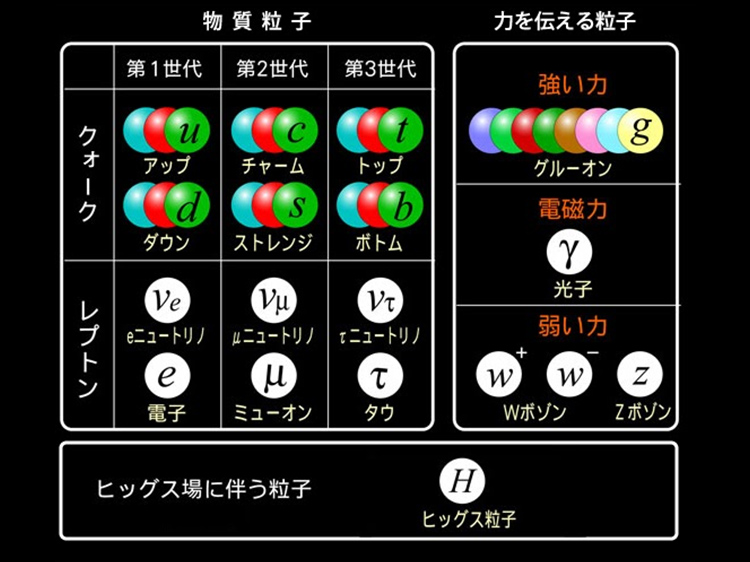
\includegraphics[clip, width=11cm]{fig/1/standardmodel_v2.jpg}
  \caption{標準模型を構成する17種類の素粒子。\cite{article:ATLAS_japan}}
  \label{fig:1-1}
\end{figure}

\newpage

標準模型は多くの実験結果を説明することのできる非常に優れた物理理論であるが、ヒッグスの階層性や宇宙・天体観測から存在がわかっている暗黒物質の正体など標準模型で説明できない問題が多く残っている。
そこで、これらの問題を解決するために世界中で様々な素粒子実験が行われている。

欧州原子核研究機構~(CERN)\cite{article:CERN}によって建設された~Large~Hadron~Collider~(LHC)\cite{article:LHC}を用いた素粒子実験である~ATLAS実験\cite{article:ATLAS}もその1つである。

ATLAS実験では、標準模型の精密測定に加えて超対称性粒子など標準模型を超えた物理現象の解明を目指し世界最高エネルギーでの高エネルギー素粒子実験が行われている。

LHC及びATLAS検出器は2018年から2022年までアップグレードが行われ、2022年7月から陽子陽子衝突の重心系エネルギー~($\sqrt{s}=13.6$)TeVで第三期運転~(Run-3)としてデータ取得が開始された。これまでほかの実験では到達できていないエネルギー領域において、新たな発見を目指す。
\chapter{LHC-ATLAS実験}
\label{chapter2}

LHC-ATLAS 実験は、LHC (Large Hadron Collider)を用いた陽子–陽子衝突によって生成された粒子を ATLAS (A Troidal LHC ApparatuS)検出器によって検出し、標準模型の精密測定や新粒子探索などを行う実験である [5]。LHC は 2018 年に Run-2 を終了し、2019 年から 2021 年にかけて LHC 及び ATLAS 検出器のアップグレードが行われ、2022 年から Run-3 が開始された。

\section{LHC加速器}
\label{section2-1}

Large Hadron Collider (LHC)は、スイスのジュネーブ郊外にある欧州素粒子原子核研究機構 (CERN)の地下に建設された周長約 27 km の世界最大の大型ハドロン衝突型加速器である。LHC加速器の概略図を図\ref{fig:LHC加速器}に示す。
LHC加速器では高いエネルギーで陽子を衝突させることにより、TeV スケールまでの物理事象を広く調べることを目的とし様々な実験を行っている。

\begin{figure}[tb]
  \centering
  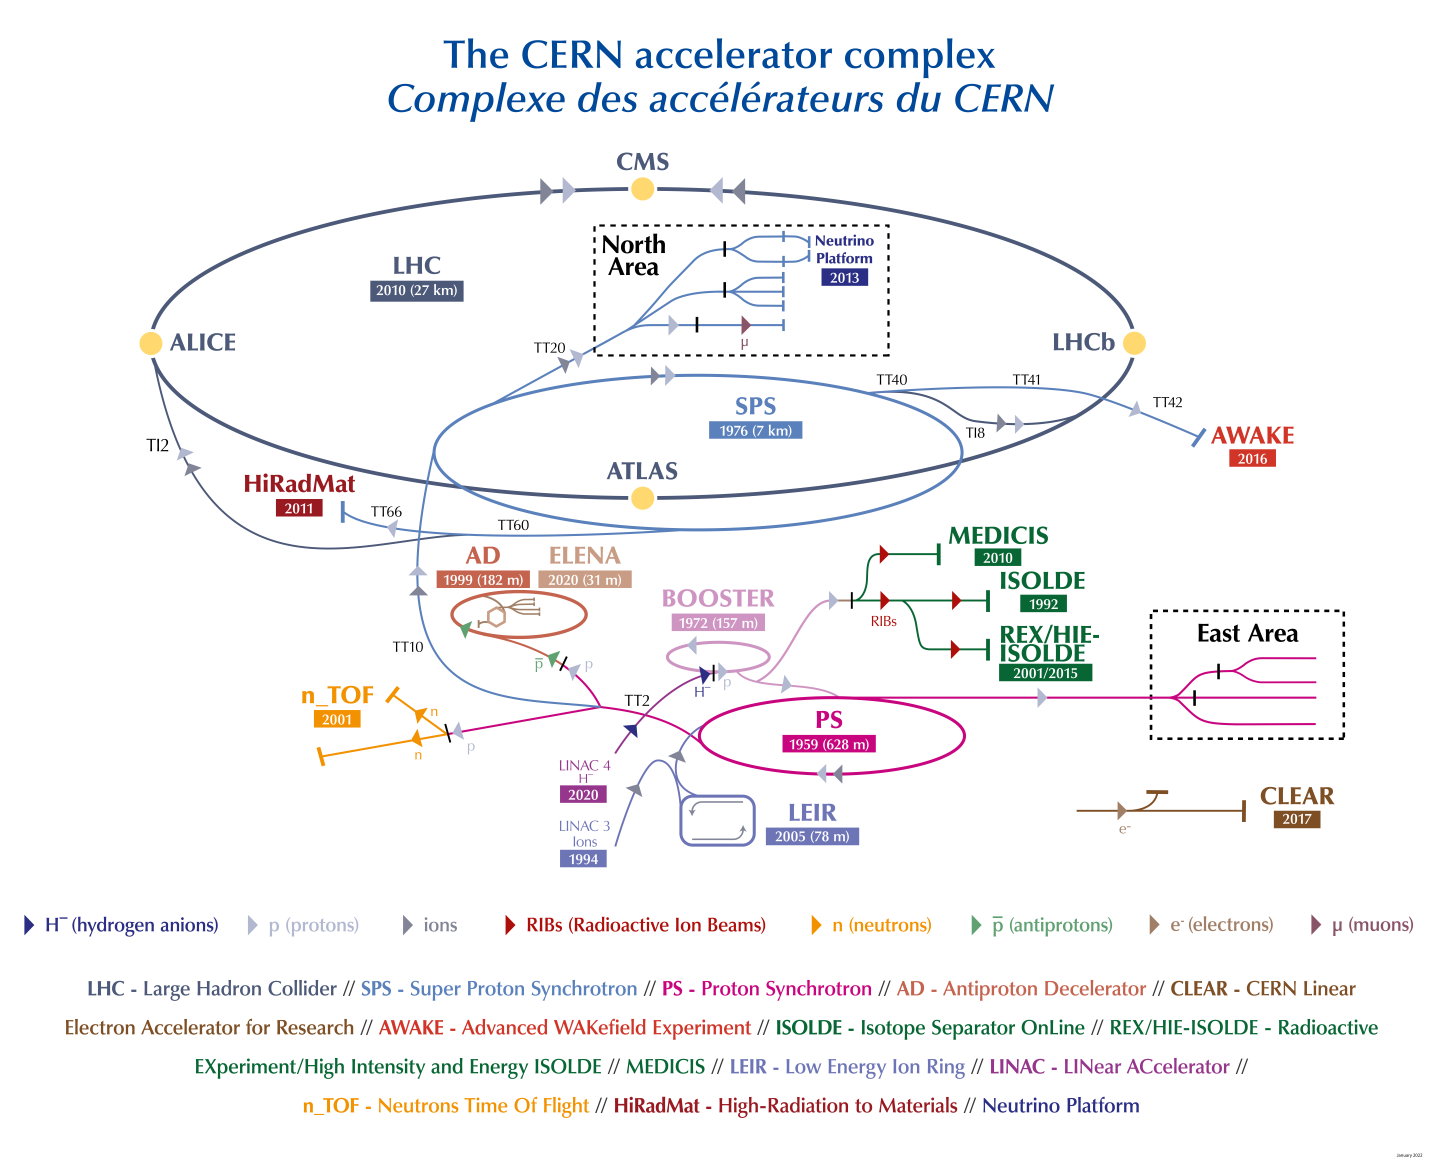
\includegraphics[clip]{fig/2/accel_complex-v2022_complex.png}
  \caption{LHC加速器の概略図}
  \label{fig:LHC加速器}
\end{figure}


LHCに陽子ビームを入射する前に、いくつかの前段加速器を使用し加速される。
初めに線源からの陽子は 線形加速器である LINAC2 で 50MeV まで加速される。第二段階は、Proton Synchrotron Booster (PSB) で1.4GeVまで加速される。Proton Synchrotron (PS) でビームを26GeVまで加速し、40MHzのバンチ構造を形成する。
その後、Super Proton Synchrotron (SPS) で450GeVまで加速された後、ビームはLHCに入射される。
LHCは陽子ビームが反対方向に周回するための2つのリングから構成されており、4か所ある衝突点にそれぞれ検出器が設置されている。
その衝突点の一つにATLAS 検出器が設置され、陽子同士の衝突から生成される粒子を検出する。
 他3箇所にも検出器が設置されており、それぞれCMS(Compact Muon Solenoid)、LHCb (Large Hadron Collider b)、ALICE (A Large Ion Collider Experiment)である。
 ATLAS と CMS の2つの検出器は、標準模型の検証から標準模型を超える現象の探索まで可能な汎用検出器である。
 LHCb と呼ばれる検出器は、B-ハドロン系の物理を研究するために設計されたものである。
 最後の ALICE は、QCD 現象を探るために重イオン衝突の研究に最適化された検出器である。

LHC

\section{ATLAS実験}
\label{section2-2}
\subsection{ATLAS検出器}
ATLAS検出器は、LHCの衝突点の1つに設置された、直径25m、長さ44mの円筒形の大型汎用検出器である。
ATLAS検出器は複数の検出器を組み合わせて構成されており、内側から内部飛跡検出器、カロリメータ、ミューオンスペクトロメータといった検出器が設置されている。また、内部飛跡検出器とカロリメータの間には超電導ソレノイド磁石、カロリメータの外側にはトロイド磁石がそれぞれ設置されており、磁場によって曲げられた荷電粒子の曲率半径から運動量の算出を行っている。

\begin{figure}[tb]
  \centering
  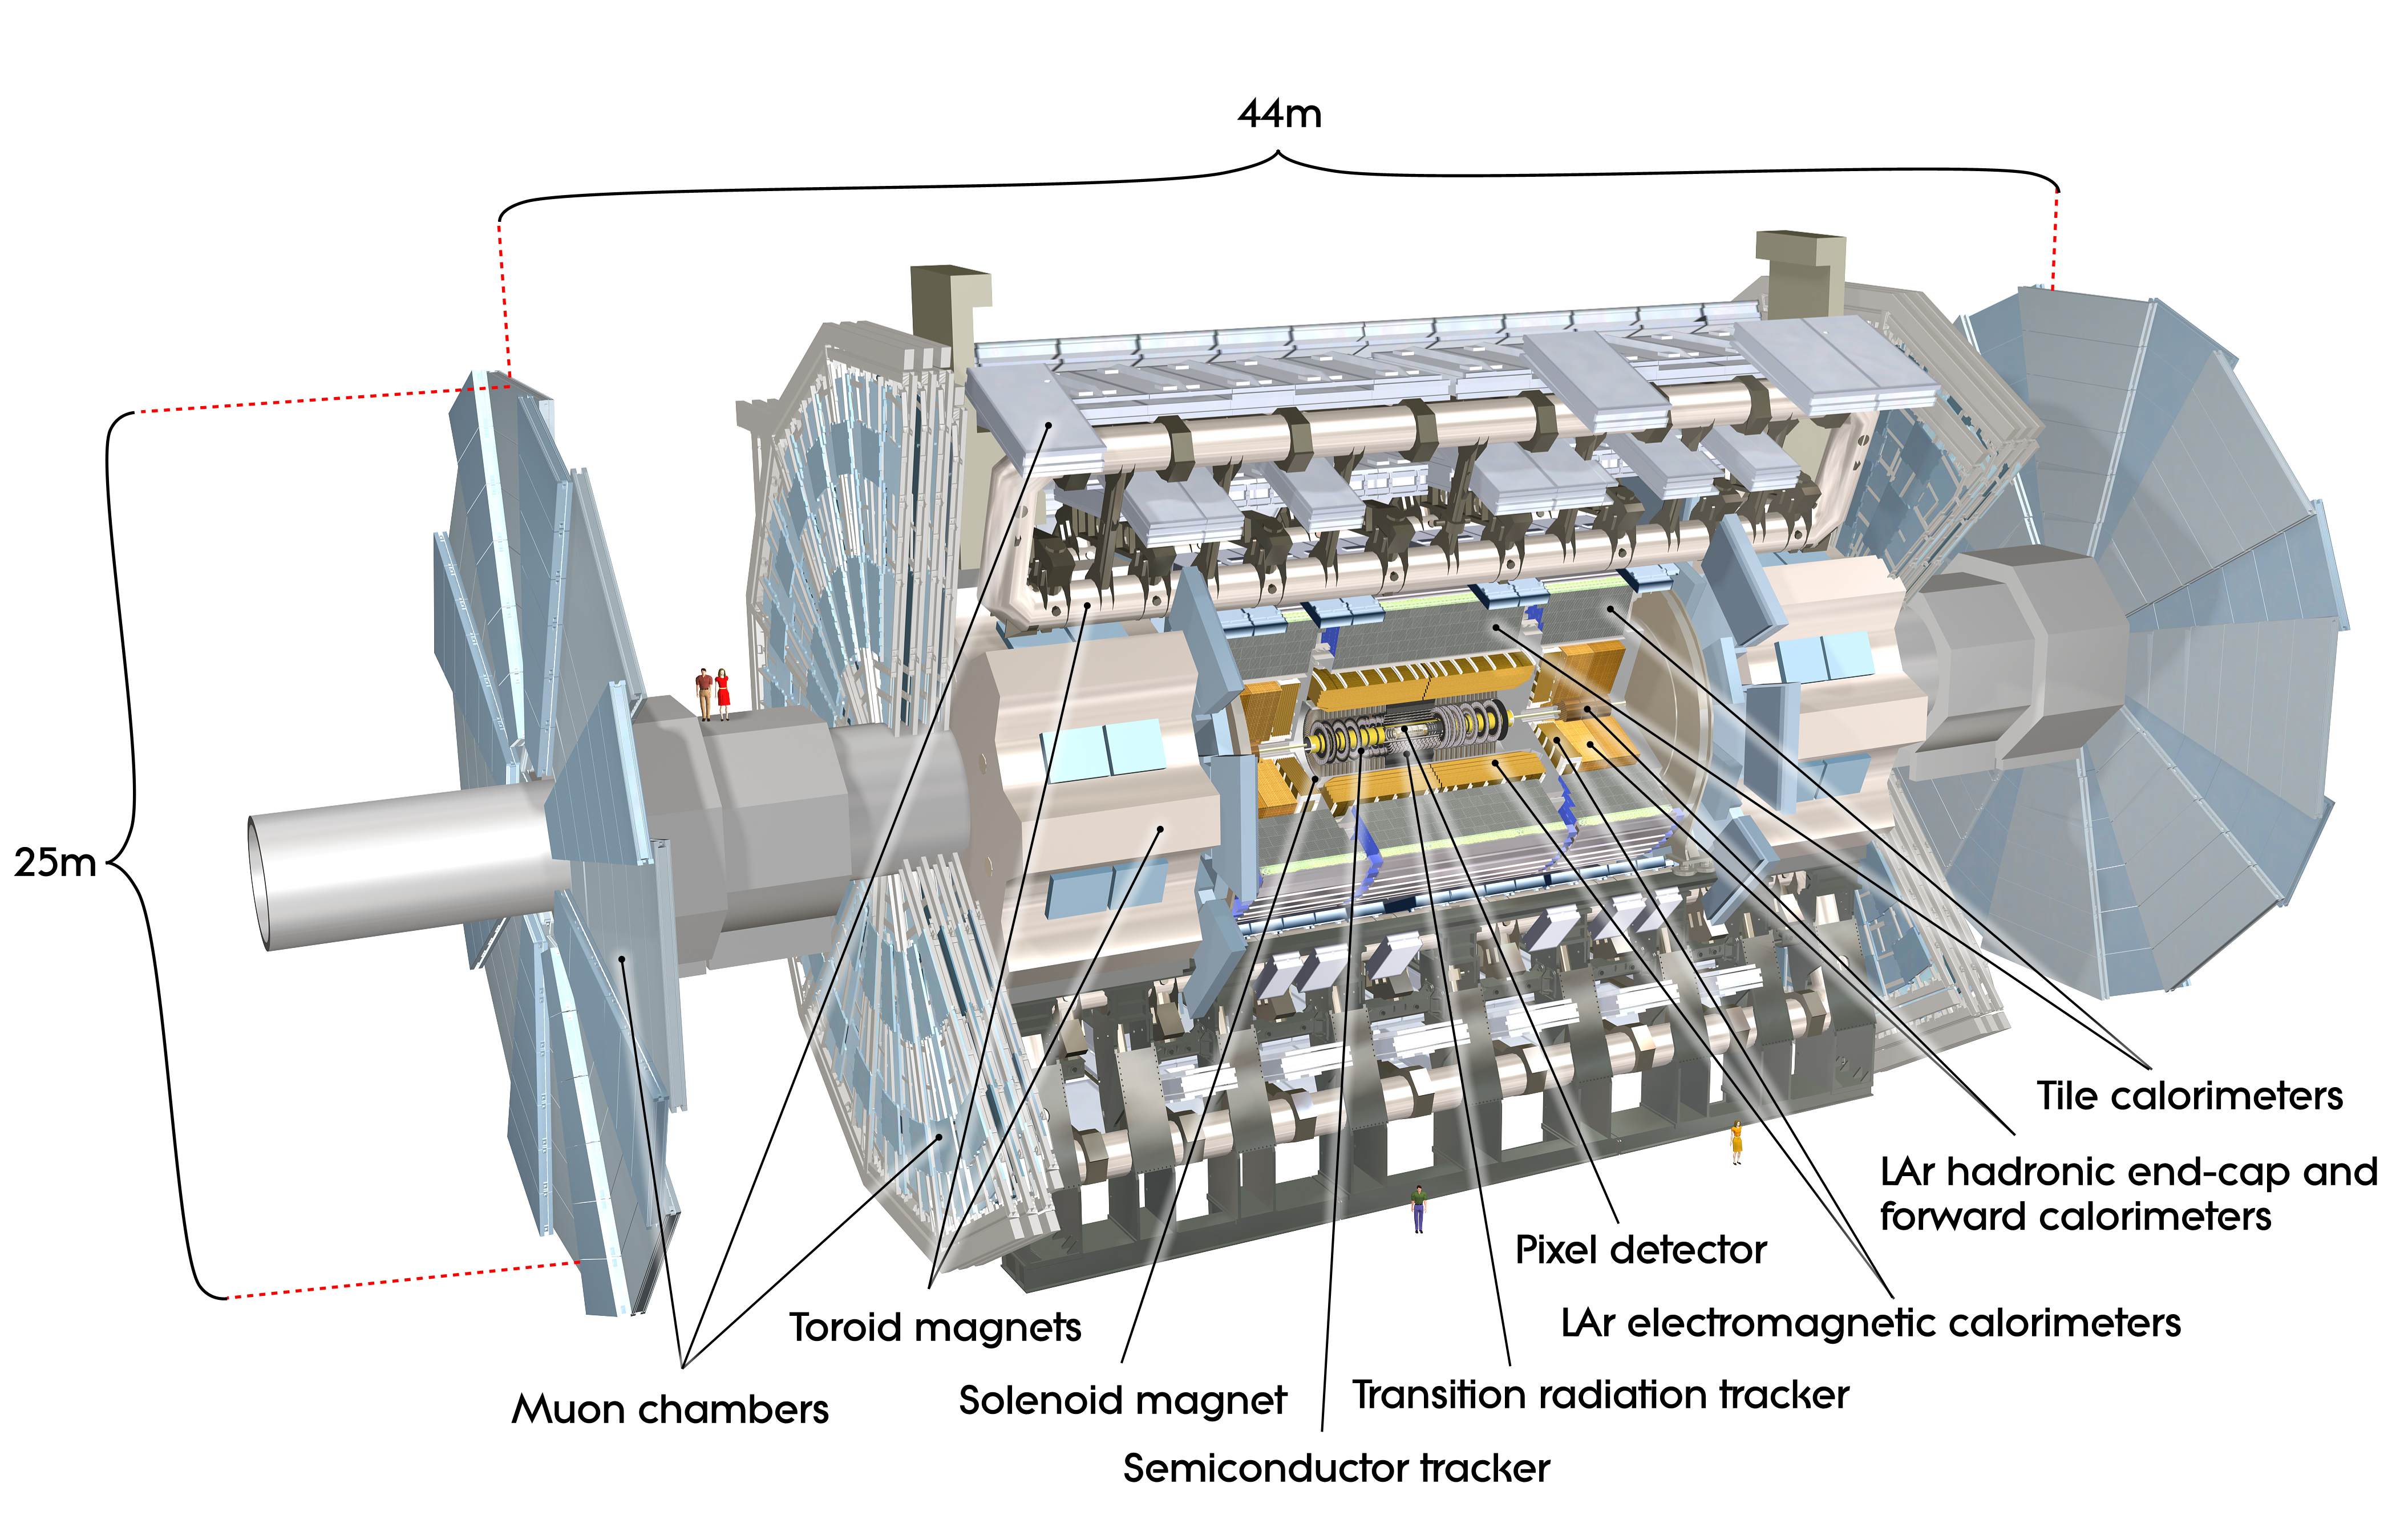
\includegraphics[clip,width=14cm]{fig/2/0803012_01.jpg}
  \caption{ATLAS検出器の全体図}
  \label{fig:ATLAS検出器}
\end{figure}


\subsection{ATLAS検出器における座標系}
ATLAS検出器における座標系を示す(図\ref{fig:a})。検出器の中心を原点とし、ビーム軸に沿ってz軸を取る。地面に対して平行方向にx軸を取り、垂直方向にy軸を取る直行座標系および、円筒座標系を設定する。また、ATLAS実験では、$\eta=-ln(tan\theta/2)$と定義される擬ラピディティ$\eta$を使用する。

\begin{figure}[tb]
  \centering
  \includegraphics[clip, width=14cm]{fig/2/atlas_coordinate_fix.pdf}
  \caption{ATLAS検出器における座標系}
  \label{fig:a}
\end{figure}

衝突点を原点とし、ビーム軸に沿ってz軸を取る。地面に水平方向にx軸を取り、x-z平面に垂直方向にy軸を取る。

\subsection{内部飛跡検出器}

\begin{figure}
    \centering
    \begin{minipage}[b]{0.3\linewidth}
        \centering
        \includegraphics[clip, width=8cm]{fig/2/inner_detectoer1.jpg}
        \vspace{10pt}
        \subcaption{内部飛跡検出器の概略図}
        \label{fig:内部飛跡検出器の概略図1}
    \end{minipage}
    \hfill
    \begin{minipage}[b]{0.5\linewidth}
        \centering
        \includegraphics[clip, width=7cm]{fig/2/inner_detector2.jpg}
        \vspace{10pt}
        \subcaption{内部飛跡検出器の概略図}
        \label{fig:内部飛跡検出器の概略図2}
    \end{minipage}
    \caption{Three simple graphs}
    \label{fig:three graphs}
\end{figure}



\subsection{カロリメータ}
カロリメータは、内部飛跡検出器の外側に設置されており、LHCでの陽子衝突で生成された粒子のエネルギー及び位置を測定する役割を担っている。
ATLAS検出器に設置されているカロリメータは、吸収層と検出層からなるサンプリングカロリメータであり、高密度物質の吸収層で粒子シャワーを起こし、検出層で電気信号に変えることで粒子の同定を行っている。
ATLASのカロリメータは、電磁カロリメータとハドロンカロリメータの2種類設置されている。

\subsubsection{・電磁カロリメータ}
電磁カロリーメーターは、$|\eta|<1.5$をカバーするバレルカロリメータと、$1.4<|\eta|<3.4$をカバーするエンドキャプカロリメータに分かれている。
バレル部とエンドキャプ部ともに、吸収層の鉛と検出層の液体アルゴンで構成されたカロリメータであり、電磁相互作用を起こす光子や電子のエネルギーと位置を測定する役割を担っている。

\subsubsection{・ハドロンカロリメータ}
ハドロンカロリメータは電磁カロリメータの外側に設置されており、タイルカロリーメータ、エンドキャップカロリーメータ、フォワードカロリーメータの3つに分類され、それぞれ異なる$|\eta=$範囲をカバーする。バレル部では、鉛と

\subsection{ミューオンスペクトロメータ}
\label{section2-2-4}
バレル領域は |η| < 1.05、エンドキャップ領域は |η| > 1.05
に対応する。また、η > 0 を A-side、η < 0 を C-side と呼ぶ。


\subsubsection{・Thin Gap Chambers (TGC)}



\subsection{マグネットシステム}
\subsubsection{・ソレノイド磁石}





\chapter{初段ミューオントリガーシステム}
ATLAS 実験におけるミューオントリガーは、RPC を用いるバレル部と TGC を用いるエンドキャップ部に分かれている。
本章では、Run-3 におけるエンドキャプ部初段ミューオントリガーシステムについて述べる。

\section{エンドキャプ部初段ミューオントリガー}
ATLAS 実験におけるミューオントリガーに用いる検出器は、図\ref{fig:muon}に示すように RPC を用いるバレル部と TGC を用いるエンドキャップ部に分かれている。以下では TGC を用いるエンドキャップ部でのトリガーシステムについて説明する。エンドキャプ部はさらに2つの領域に分けられ、$1.05 < |\eta| < 1.9$ をエンドキャップ領域、$1.9 < |\eta| < 2.4$ をフォワード領域と呼ぶ。
\begin{figure}[tb]
  \centering
  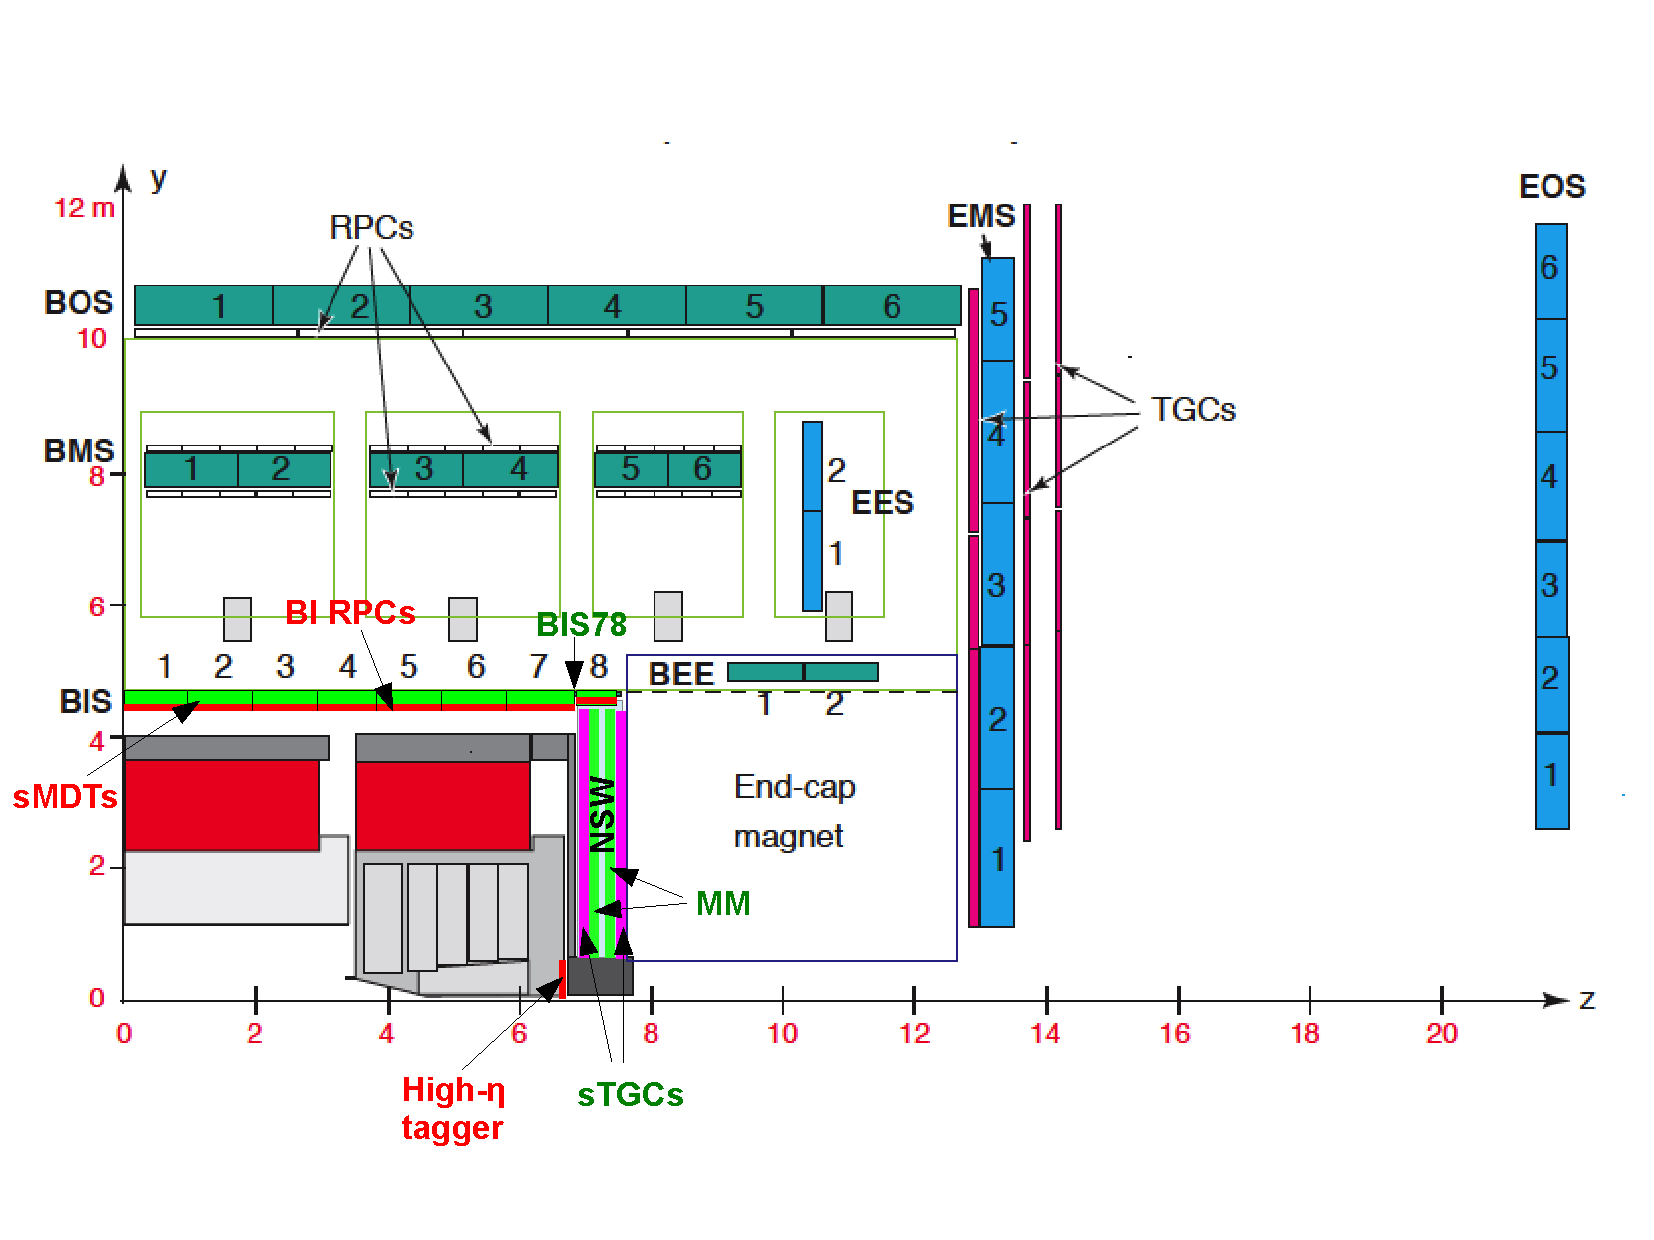
\includegraphics[clip, width=14cm]{fig/2/ch01_fig_03a.pdf}
  \caption{初段ミューオントリガーに用いる検出器の設置位置。}
  \label{fig:muon}
\end{figure}

\subsection{ミューオントリガーの概要}\label{section:CW}
エンドキャップ部の初段ミューオントリガーで用いられるトリガー判定の概要を図\ref{fig:trigger-scheme}に示す。
衝突点で生成されたミューオンはトロイド磁石の磁場領域より内側にある検出器を通過した後、トロイド磁場領域を通り TGC に到達する。トロイド磁石による磁場は $\phi$ 方向にかかっているため、ミューオンの飛跡はトロイド磁場中で$\eta$ 方向に曲げられる。さらに、衝突点付近のソレノイド磁石で生じる $z$ 方向の磁場成分と、トロイド磁石付近で生じた $R$ 方向の磁場成分によって、ミューオンの飛跡は $\phi$ 方向にも曲げられる。ミューオンの飛跡の曲がり具合は 横方向運動量$p_T$ の大きさによって変化するため、飛跡情報からミューオンの$p_T$を算出することができ、トリガー判定に使用することができる。

トロイド磁場によって曲げられたミューオンは TGC BW の M1, M2, M3 を通過し、ヒット情報から飛跡を再構成される。ここで、衝突点と M3 のヒット位置を結んだ直線をミューオンが無限運動量で通過したと仮定した場合の飛跡として扱う。この無限運動量を持つミューオンの飛跡と磁場によって曲げられた実際の飛跡を比較し、M1 におけるヒット位置の $R$ 方向と $\phi$ 方向のずれ ($dR$, $d\phi$) を計算する。この ($dR$, $d\phi$) は磁場による飛跡の曲がり具合を表している。
この $dR$ と $d\phi$ の値が大きいミューオンは、磁場中で大きく曲げられたことを意味しており、小さい $p_T$ として判定される。逆に $dR$ と $d\phi$ の値がが小さいほど、磁場中ではあまり曲がらないミューオンの飛跡であるため、大きな $p_T$ として判定される。
そして、事前に ($dR$, $d\phi$) に対応する $p_T$ の関係を Look-Up Table (LUT) として保存しておき、トリガー判定の際に LUT を参照する事で短時間での $p_T$ の出力を可能としている。

\begin{figure}[tb]
  \centering
  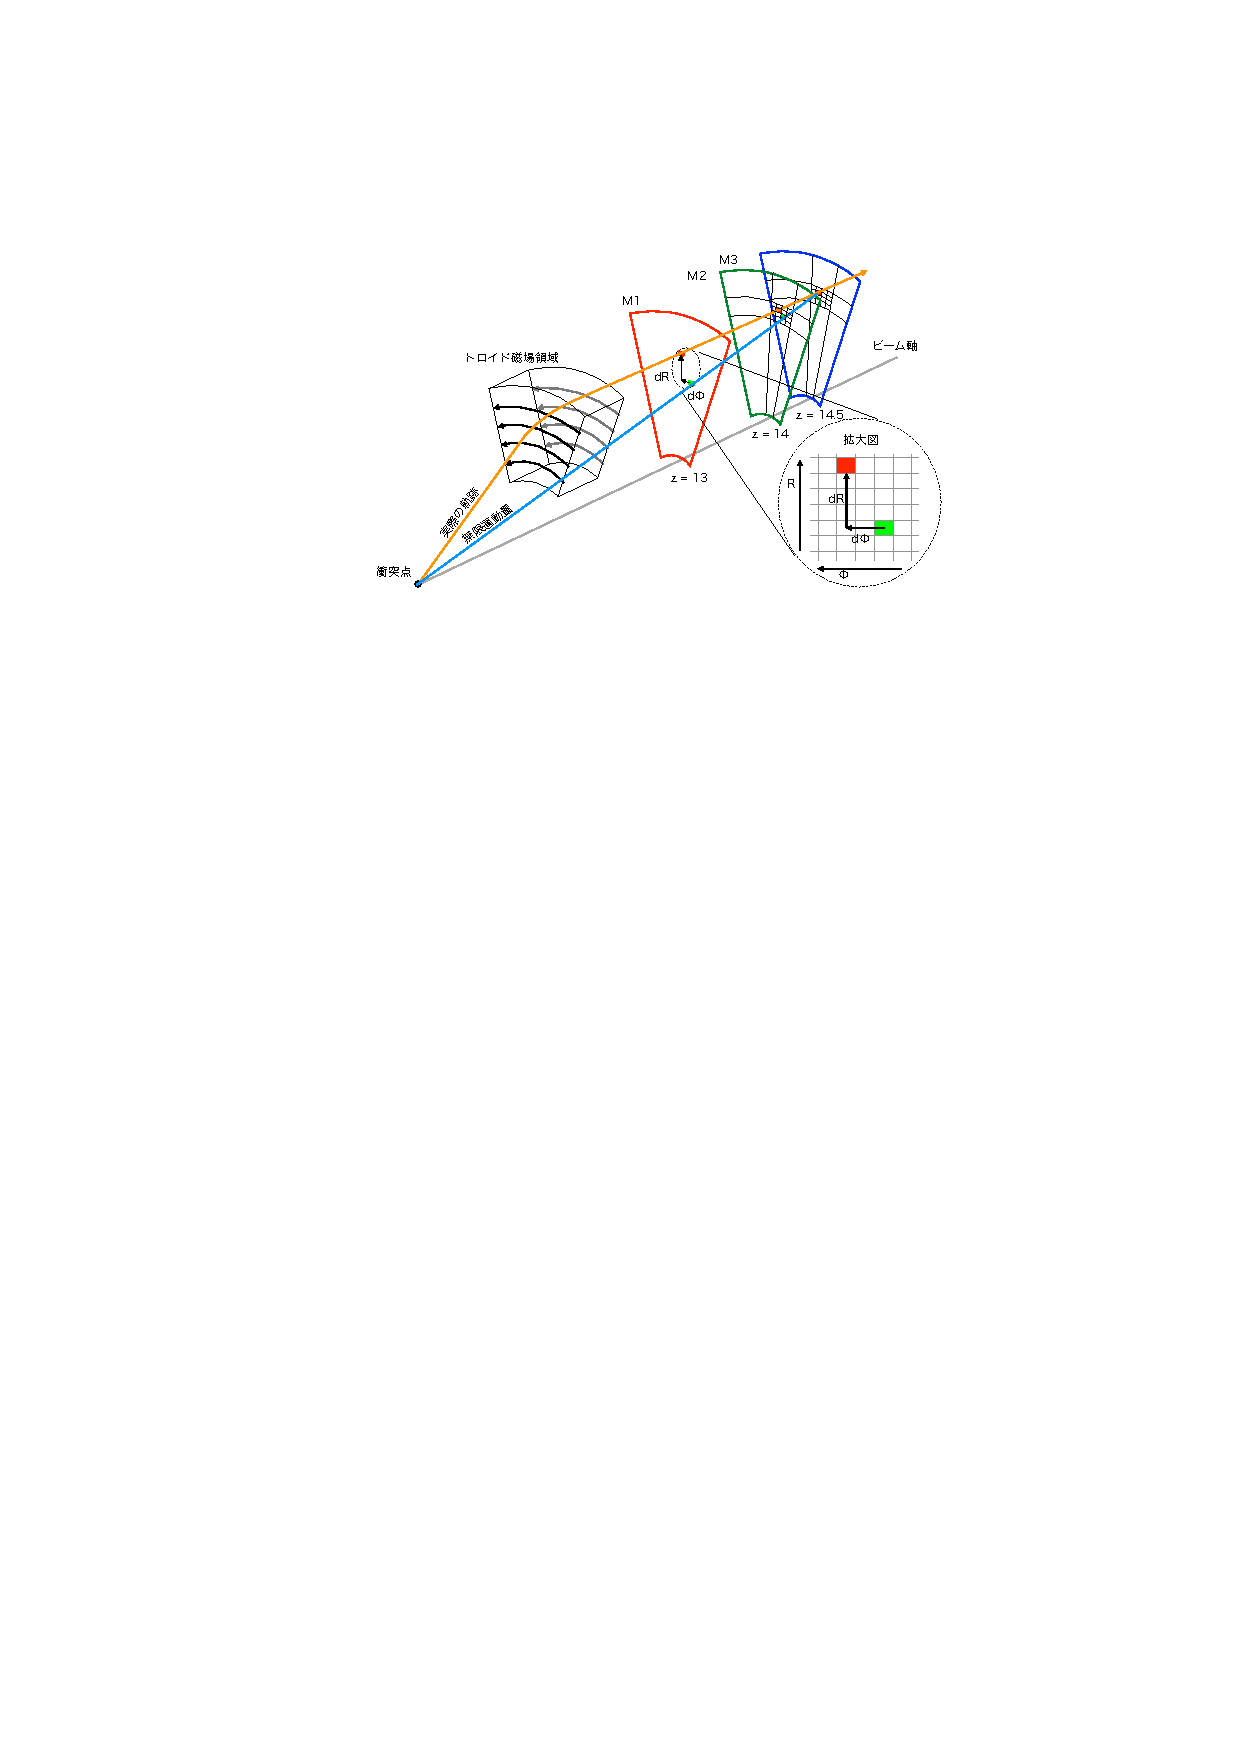
\includegraphics[clip, width=15cm]{fig/3/akatsuka_mt_trigger_scheme.pdf}
  \caption{ATLAS検出器エンドキャップ領域におけるトリガースキームの概念図\cite{article:akatsuka-mron}。無限大の運動量を持つミューオンを仮定し、磁場によって曲げられたミューオンとの位置の差 ($dR$, $d\phi$) を用いて$p_T$を計算する。}
  \label{fig:trigger-scheme}
\end{figure}

LUT とは入力データに対応する出力データを参照するための表のことを指し、初段ミューオントリガーでは、($dR$, $d\phi$) を入力として $p_T$ を出力する LUT を FPGA に保存している。

\subsubsection{coincidence Window}
この LUT は Coincidence Window (CW) と呼ばれており、初段ミューオントリガーでは事前にシミュレーションデータを用いて ($dR$, $d\phi$) に対応する $p_T$ を算出し、Run-3では図\ref{fig:CW}のように 15 段階の $p_T$ 閾値を判定できる形式でで FPGA に保存している。

Run-3 で使用される CW は図\ref{fig:CW}の色のように 15 個に分類されている。この各色が 15 段階の $p_T$ 閾値に対応しており、マスの中の数字は表\ref{pt_number} に示す $p_T$ number と対応している。また、各 $p_T$ 閾値の符号はミューオンの電荷に対応している。図\ref{fig:CW}の
エンドキャップ部のトロイド磁場や TGC は理想的には 8 回対称であるが、磁場の向きや TGC チェンバーの設置位置のズレなどがあるため、CW は TGC-BW のトリガー判定に用いられる単位位置情報ごとに独立に作成されている。


\begin{figure}[tb]
  \centering
  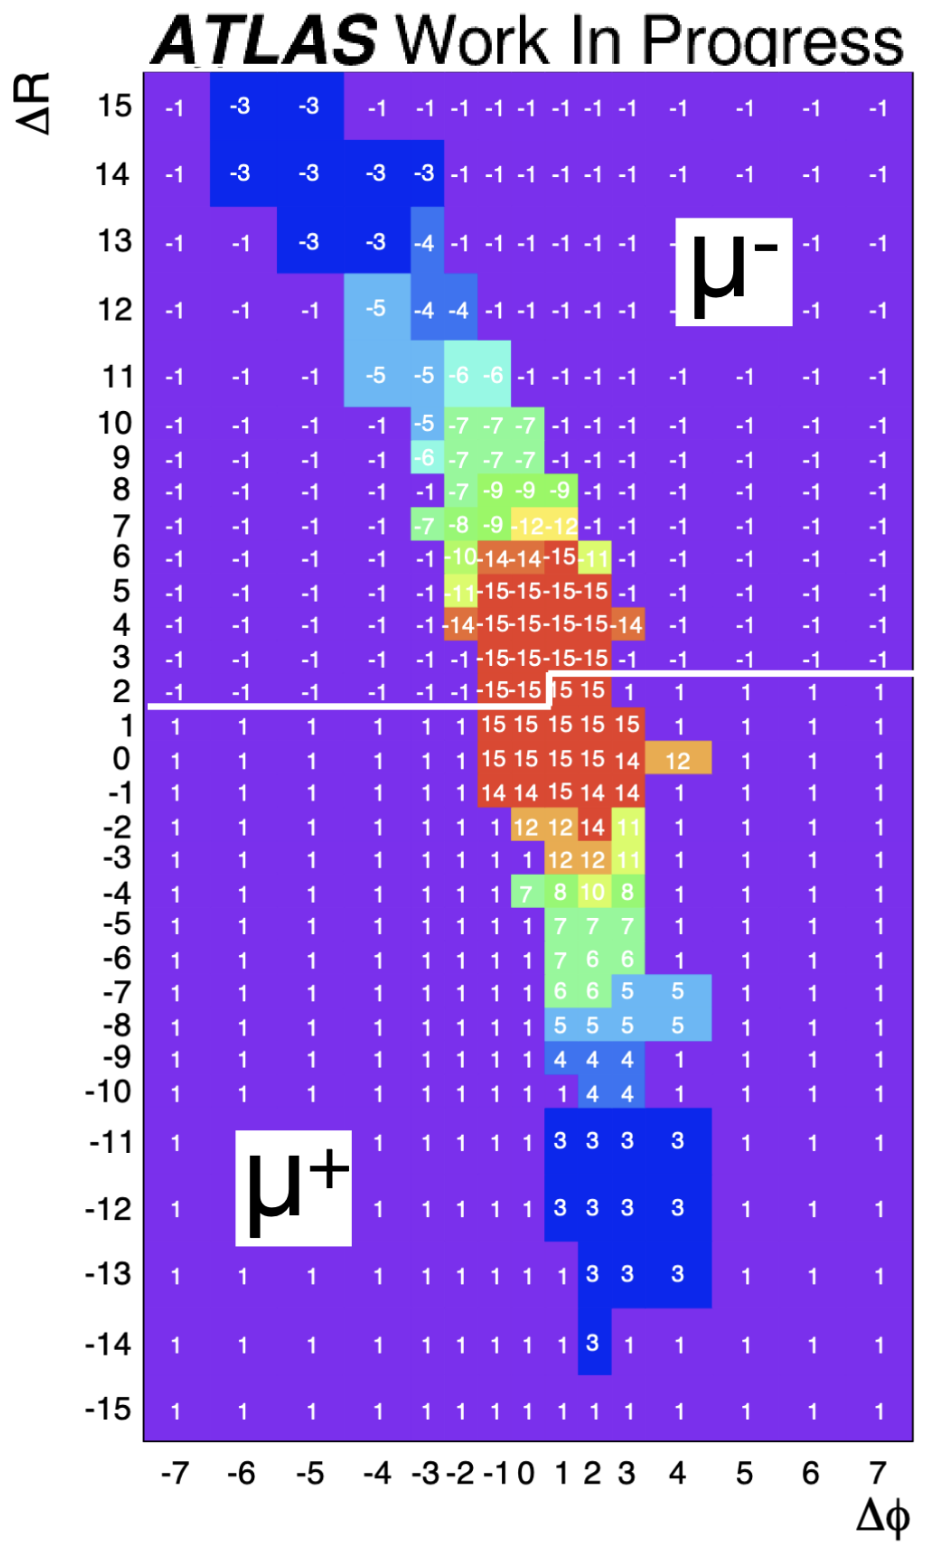
\includegraphics[clip, width=7cm]{fig/3/cw_run3_shiomi.png}
  \caption{Run-3 での TGC における Coincidence Window の例。ミューオンのヒットがあった時にそれぞれの検出位置のの CW を参照し、$dR$、$dφ$ からミューオンの $p_T$ を 15 段階で見積もる。}
  \label{fig:CW}
\end{figure}

\begin{table}[]
    \caption{Run-3 初段ミューオントリガーにおける 15 段階の $p_T$ 閾値。}
    \label{pt_number}
    \centering
    %\begin{tabular}{|c|c|c|c|c|c|c|c|c|c|c|c|c|c|c|c|c|c|c|c|c|c|c|c|}
    \begin{tabular}{|c|c|c|c|}
        \hline
        $p_T$ number & Threshould name & Status\\
        \hline
        1 & L1$\_$MU3 & $p_T \geq$ 3 GeV \\
        \hline
        2 & L1$\_$MU4 & $p_T \geq$ 4 GeV \\
        \hline
        3 & L1$\_$MU5 & $p_T \geq$ 5 GeV \\
        \hline
        4 & L1$\_$MU6 & $p_T \geq$ 6 GeV \\
        \hline
        5 & L1$\_$MU7 & $p_T \geq$ 7 GeV \\
        \hline
        6 & L1$\_$MU8 & $p_T \geq$ 8 GeV \\
        \hline
        7 & L1$\_$MU9 & $p_T \geq$ 9 GeV \\
        \hline
        8 & L1$\_$MU10 & $p_T \geq$ 10 GeV \\
        \hline
        9 & L1$\_$MU11 & $p_T \geq$ 11 GeV \\
        \hline
        10 & L1$\_$MU12 & $p_T \geq$ 12 GeV \\
        \hline
        11 & L1$\_$MU13 & $p_T \geq$ 13 GeV \\
        \hline
        12 & L1$\_$MU14 & $p_T \geq$ 14 GeV \\
        \hline
        13 & L1$\_$MU15 & $p_T \geq$ 15 GeV \\
        \hline
        14 & L1$\_$MU18 & $p_T \geq$ 18 GeV \\
        \hline
        15 & L1$\_$MU20 & $p_T \geq$ 20 GeV \\
        \hline
        %$p_t$ number & 1 & 2 & 3 & 4 & 5 & 6 & 7 & 8 & 9 & 10 & 11 & 12 & 13 & 14 & 15\\
        %\hline
        %$p_T$ Threshould[GeV] & 3 & 4 & 5 & 6 & 7 & 8 & 9 & 10 & 11 & 12 & 13 & 14 & 15 & 18 & 20\\
        %$p_T$ Threshould & 3 & 4 & 5 & 6 & 7 & 8 & 9 & 10 & 11 & 12 & 13 & 14 & 15 & 18 & 20\\
        %\hline
    \end{tabular}
\end{table}

また、CW にはコインシデンスのタイプによって 4 種類存在する。
一つ目は M1 から M3 まで 3 つのステーション (M1, M2, M3) 全てにおいてワイヤーとストリップともにヒットが確認された 3-3 ステーションコインシデンス、二つ目がワイヤーは 3 ステーションにヒットが確認されたが、ストリップに関しては 2 ステーション (M2, M3) のヒットのみしか確認できなかった 3-2 ステーションコインシデンス、三つ目がワイヤーは2 ステーション  にしかヒットが確認されなかったが、ストリップでは 3 ステーションにヒットが確認された 2-3 ステーションコインシデンス、四つ目がワイヤーとストリップともに 2 ステーションしかヒットが確認できなかった 2-2 ステーションコインシデンスである。
3 ステーションコインシデンスフラグはストリップ、ワイヤー共に 3 ステーションでヒットがあった場合に立つフラグである。2 ステーションコインシデンスか 3 ステーションコインシデンスかでズレを計算するヒット位置がM2-M3 か、M1-M3 か変わってくるため、dR、dφ の範囲も変わってくる。2 ステーションの場合、$−7 \geq dR \geq 7$、$−3 \geq d\phi \geq 3$、3 ステーションの場合、$−15 \geq dR \geq 15$、$−7 \geq d\phi \geq 7$ の範囲で定義される。


\subsubsection{トリガーセクター}
TGC のトリガー判定に用いられる単位の模式図を図\ref{fig:RoI}に示す。TGC のトリガー判定はトリガーセクターごとに行われ、領域内のミューオンの情報から判定結果が出される。
エンドキャップ部のトリガーセクターは、 $\phi$ 方向にエンドキャプ領域では 48 個、フォワード領域では 24 個に分割している。
これらのトリガーセクターはさらに小さな領域である Region of Interest (RoI) に分割される。
図\ref{fig:RoI} に示すように、エンドキャップ領域のトリガーセクターは $\eta$ 方向に 37 分割、$\phi$ 方向に 4 分割されるため 148 個の RoI で構成されている。フォワード領域のトリガーセクターは $\eta$ 方向に 16 分割、$\phi$ 方向に 4 分割されるため 64 個の RoI で構成されている。また RoI を $\eta$ 方向に 2 つ、$\phi$ 方向に 4 つまとめたものを Sub Sector Cluster (SSC) と呼ぶ。RoI は TGC の持つミューオンの検出位置情報の最小単位であり、$p_T$ 判定に用いる CW はこの RoI ごとに作成している。

\begin{figure}[tb]
  \centering
  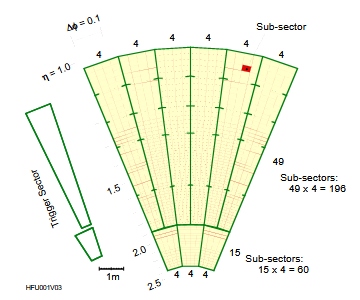
\includegraphics[clip, width=10cm]{fig/3/RoI.png}
  \caption{TGC におけるトリガーセクターと RoI の模式図。緑の線で囲まれた領域が 1 つのトリガーセクターを表し、赤の線で囲まれたマスが 1 つの RoI を表す。}
  \label{fig:RoI}
\end{figure}

\subsubsection{インナーコインシデンス}
エンドキャップ領域ミューオントリガーには衝突点由来でない荷電粒子により発行されたトリガー (フェイクトリガー) が存在し、レートを上げる要因になっている。Run-2 では TGC-EI/FI と Tile カロリメータとコインシデンス (インナーコインシデンス) を取ることでフェイクトリガーを大きく削減することができた。しかし、$1.9 < |\eta| < 2.4$ の領域ではインナーコインシデンスをとるためのトリガー用検出器がないためフェイクトリガーが多く残っている。
Run-3 からは NSW と RPC BIS78 の導入により、より広範囲のインナーコインシデンスをとることが可能になるため、フェイクトリガーをより削減できる。
Tile カロリメータとコインシデンスだけでなく、新たに導入される NSW や RPC BIS78 を用いた場合に期待されるトリガー発行数の分布を図\ref{fig:Rate_innercoincidence}に示す。

\begin{figure}[tb]
  \centering
    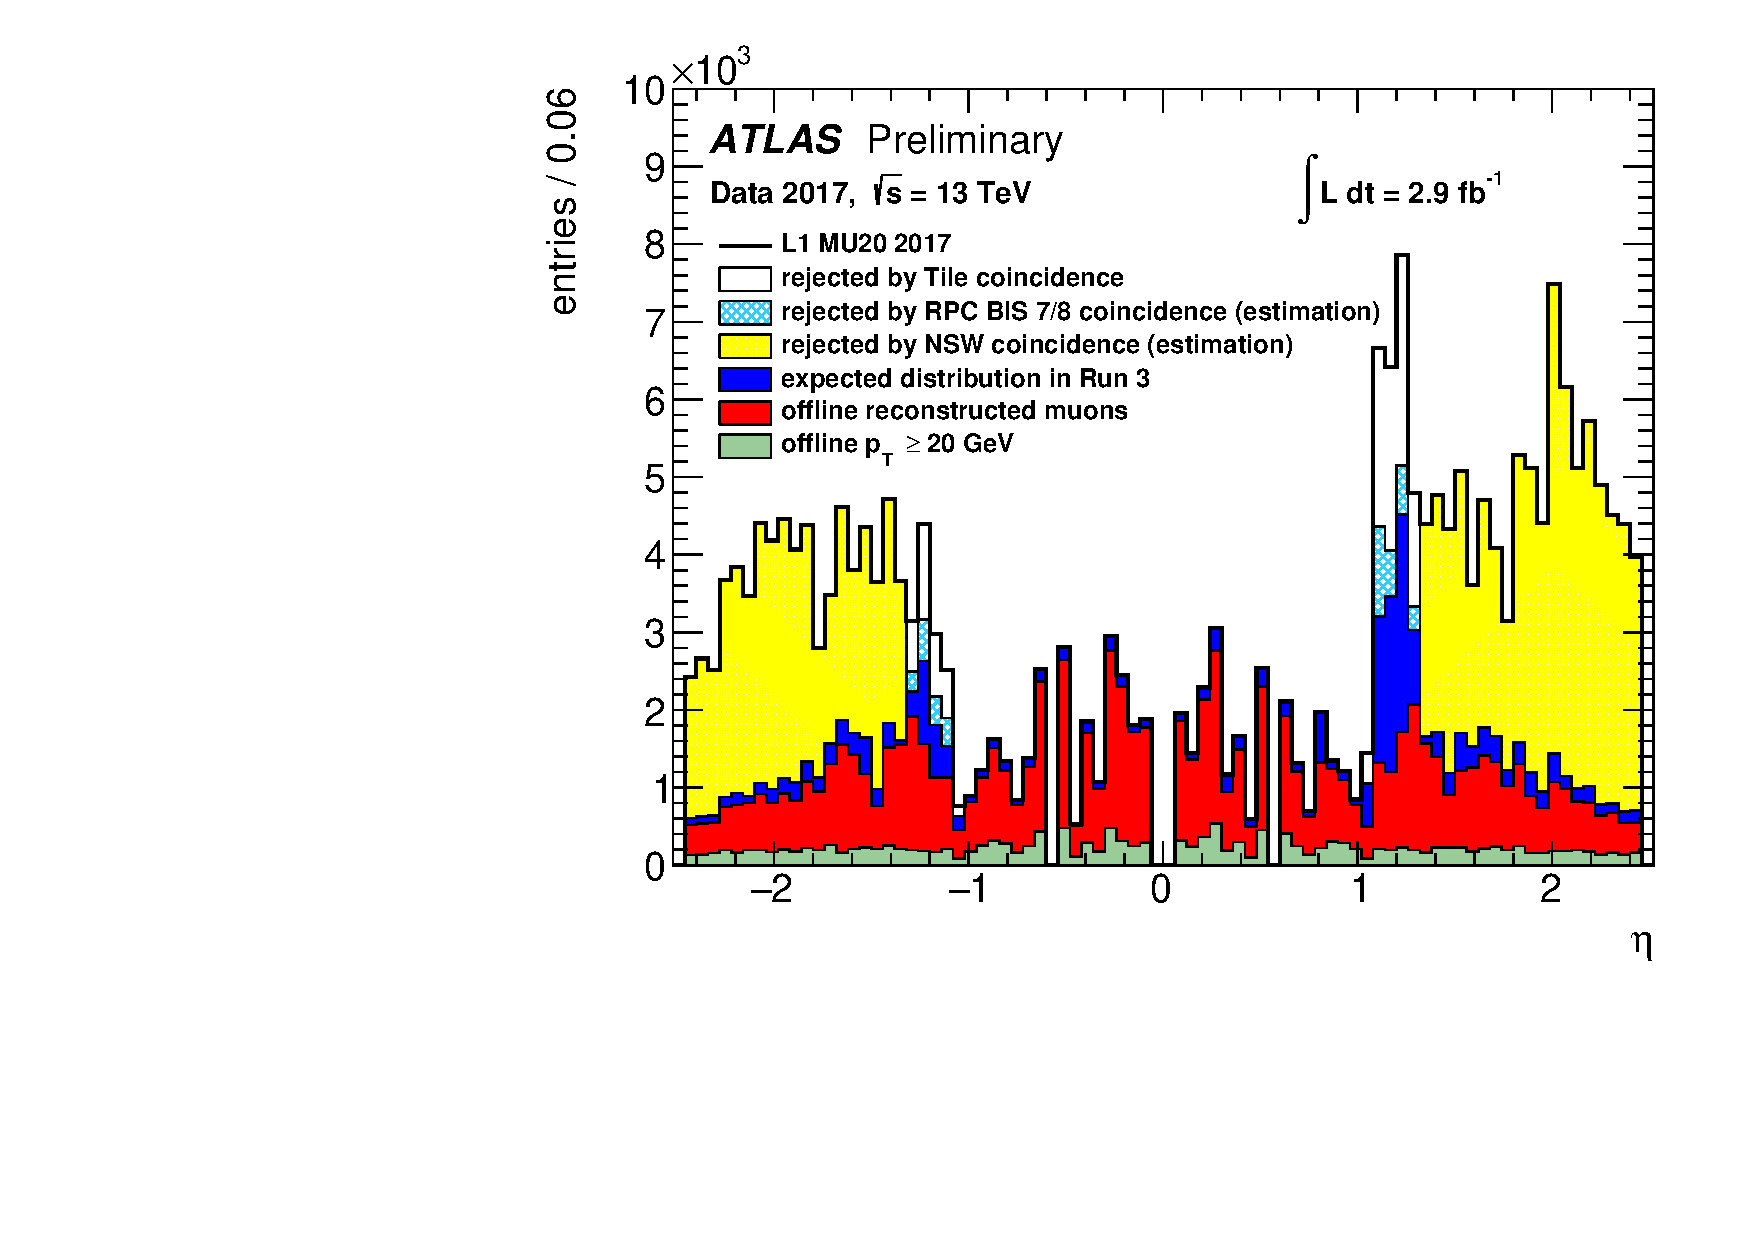
\includegraphics[clip, width=14cm]{fig/3/ATL-COM-DAQ-2018-033-fig2.pdf}
  \caption{Run-3 で期待される $p_T$ 閾値 20 GeV におけるトリガー発行数の $\eta$ 分布。白色、水色、黄色の領域はそれぞれ Tile カロリメータ、RPC BIS78、NSW を用いたインナーコインシデンスを導入した場合に削減できるトリガー発行数を示す。青色の領域は Run-3で期待されるトリガー発行数、赤色の領域は発行されたトリガーのうちオフラインで再構成されるミューオンの数を示す。緑の分布はオフラインで再構成されたミューオンのうち、$p_T$ が 20 GeV 以上のミューオンの数を示す。}
  \label{fig:Rate_innercoincidence}
\end{figure}

\subsection{初段ミューオントリガーにおけるエレクトロニクス}
初段ミューオントリガーでは、ATLAS 検出器から送られてくる情報に対して SectorLogic、MUCTPI、L1Topo、CTP という電子回路を経てトリガーが発行される。
以下では各エレクトロニクスについて説明する。

\subsubsection{Amplifier Shaper Discriminator (ASD) ボード}
Amplifier Shaper Discriminator (ASD) ボードは TGC のワイヤーとストリップからアナログ信号を受け取り、デジタル信号への変換を行う。
ASD ボード上の ASD において TGC からのアナログ信号を増幅・整形し、 閾値電圧を超えた信号のみ LVDS 信号として出力される。1 枚の ASD ボードは 4 つの ASD ASIC を搭載しており、ASD ASIC は 4 つの信号の受信・処理を行う。そのため、同時に 16 チャンネルの信号を処理することが可能である。

\subsubsection{Patch-Panel ASIC (PP ASIC)}
Patch-Panel ASIC は ASD からワイヤーとストリップそれぞれの LVDS 信号を受け取り、タイミングの調整を行うことで、同じ陽子衝突由来の信号を同時に次の SLB ASIC に送る。陽子衝突が起きてからミューオンが検出器に到達する時間や、ケーブルの長さの違いにより、信号のタイミングが各チャンネルごとに異なるため、PP ASIC を用いてタイミングの調整を行う。

\subsubsection{Slave Board ASIC (SLB ASIC)}
Slave Board ASIC は読み出しとトリガー判定の 2 種類の処理を行う。
トリガー判定で行う処理としては、各チャンネルの情報を用いてコインシデンスを取ることである。
TGC Triplet (M1 ステーション) ではワイヤーの場合は 3 層中 2 層にヒットがあることを要求し、ストリップの場合は 2 層中 1 層にヒットがあることを要求する。
2 つの TGC Doublet (M2、M3 ステーション) では、各ステーションから信号を受け取りワイヤーとストリップで独立に 4 層中 3 層以上にヒットがあることを要求する。 これらのコインシデンス結果はLVDS 信号で後段の High PT ボードに送る。

\subsubsection{High PT (HPT) ボード}
High PT ボードは、M1 の SLB と M2,M3 の SLB からのコインシデンス結果を受け取り、 M1,M2,M3 の 3つのステーション間のコインシデンスを行う。M1 と M3 の位置情報から ($\Delta R$, $\Delta \phi$) を計算し、次の Sector Logic に送る。Sector Logic にはボードごとに、位置情報 $R$ と $\phi$ 、位置の差の情報 $\Delta R$ と $\Delta \phi$ を G-Link 通信を用いて送信する。データ通信速度の制限により、1 つの HPT ASIC から最大 2 候補を選んで送信している。

\subsubsection{New Sector Logic (NSL)}
New Sector Logic では TGC-BW とトロイド磁石の内側にある検出器の情報を統合してトリガー判定を行う。
TGC-BW の HPT ボードからは、ミューオン候補の情報が G-Link 規格で送られてくる。
RPC BIS78、Tile カロリメータ、 TGC-EI からは、検出器におけるヒット情報が送られてくる。
NSW からは通過したミューオンの飛跡情報が送られてくる。
NSL はこれらの情報をもとにトリガー判定を行い、トリガー判定の結果を MUCTPI に送信する。

NSL ボードでは、 HPT ボードから受け取った TGC BW の位置情報 $R$ と $\phi$ 、位置の差の情報 $\Delta R$ と $\Delta \phi$ を用いて $p_T$ の判定を行う。各 ($R$, $\phi$) からミューオンのヒット位置を表す RoI を決定し、($\Delta R$, $\Delta \phi$) から NSL 上に実装されている Coincidence Window を用いて $p_T$ に変換する。






\section{2022年 Run-3 における初段ミューオントリガーの性能}
本節では2022年 Run-3 で使用されている CW のトリガー性能について述べる。

\subsection{解析手法}
実際の実験データはトリガーによって選別された粒子の情報のみが保存されているため、そのままのデータを用いてトリガーの性能評価や解析を行うとバイアスがかかる可能性がある。そこで解析の手法として Tag$\&$Probe 法を用いる。

本研究では、内部飛跡検出器とミューオン検出器でそれぞれ独立に再構成され、その後飛跡が結合できたZ ボソン由来のミューオン候補を用いて評価を行う。1回の衝突事象に対し、2 つ以上のミューオン候補が存在するイベントのみを用いる。それらのミューオン候補のうち、任意の2つの電荷が異符号となっているミューオンペアを選び出し、不変質量を再構成する。再構成の条件は、$80 GeV < M_Z < 100 GeV$ とする。
これらのミューオンのうち、一方を Tag ミューオン、もう一方を Probe ミューオンと定義する。
まず、Tag ミューオンがトリガーを発行したかどうかを判定する。Run-2 での実験データを解析に使用する際のトリガー判定には、HLT のシングルミューオントリガーである 「HLT$\_$mu26$\_$ivarmeduium」 を使用する。
ここでトリガー発行の判定を行うために $\Delta R = \sqrt{(\Delta \eta)2 + (\Delta \phi)2}$ を定義する。ここで $\Delta \eta$, $\Delta \phi$ はそれぞれデータの保存されているトリガーを発行した飛跡と Tag ミューオンの $\eta$ 方向、$\phi$ 方向の差である。図\ref{fig:tag_HLT}にTag ミューオンと HLT の $\Delta R$ 分布を示す。本研究では$\Delta R < 0.001$ を満たせば Tag ミューオンがトリガーを発行したとみなす。Tag ミューオンが HLT を発行しているとみなされた時、もう一つのミューオンを Probe ミューオンとして解析に使用する。

\begin{figure}[tb]
  \centering
  %\rule{8cm}{6cm}
  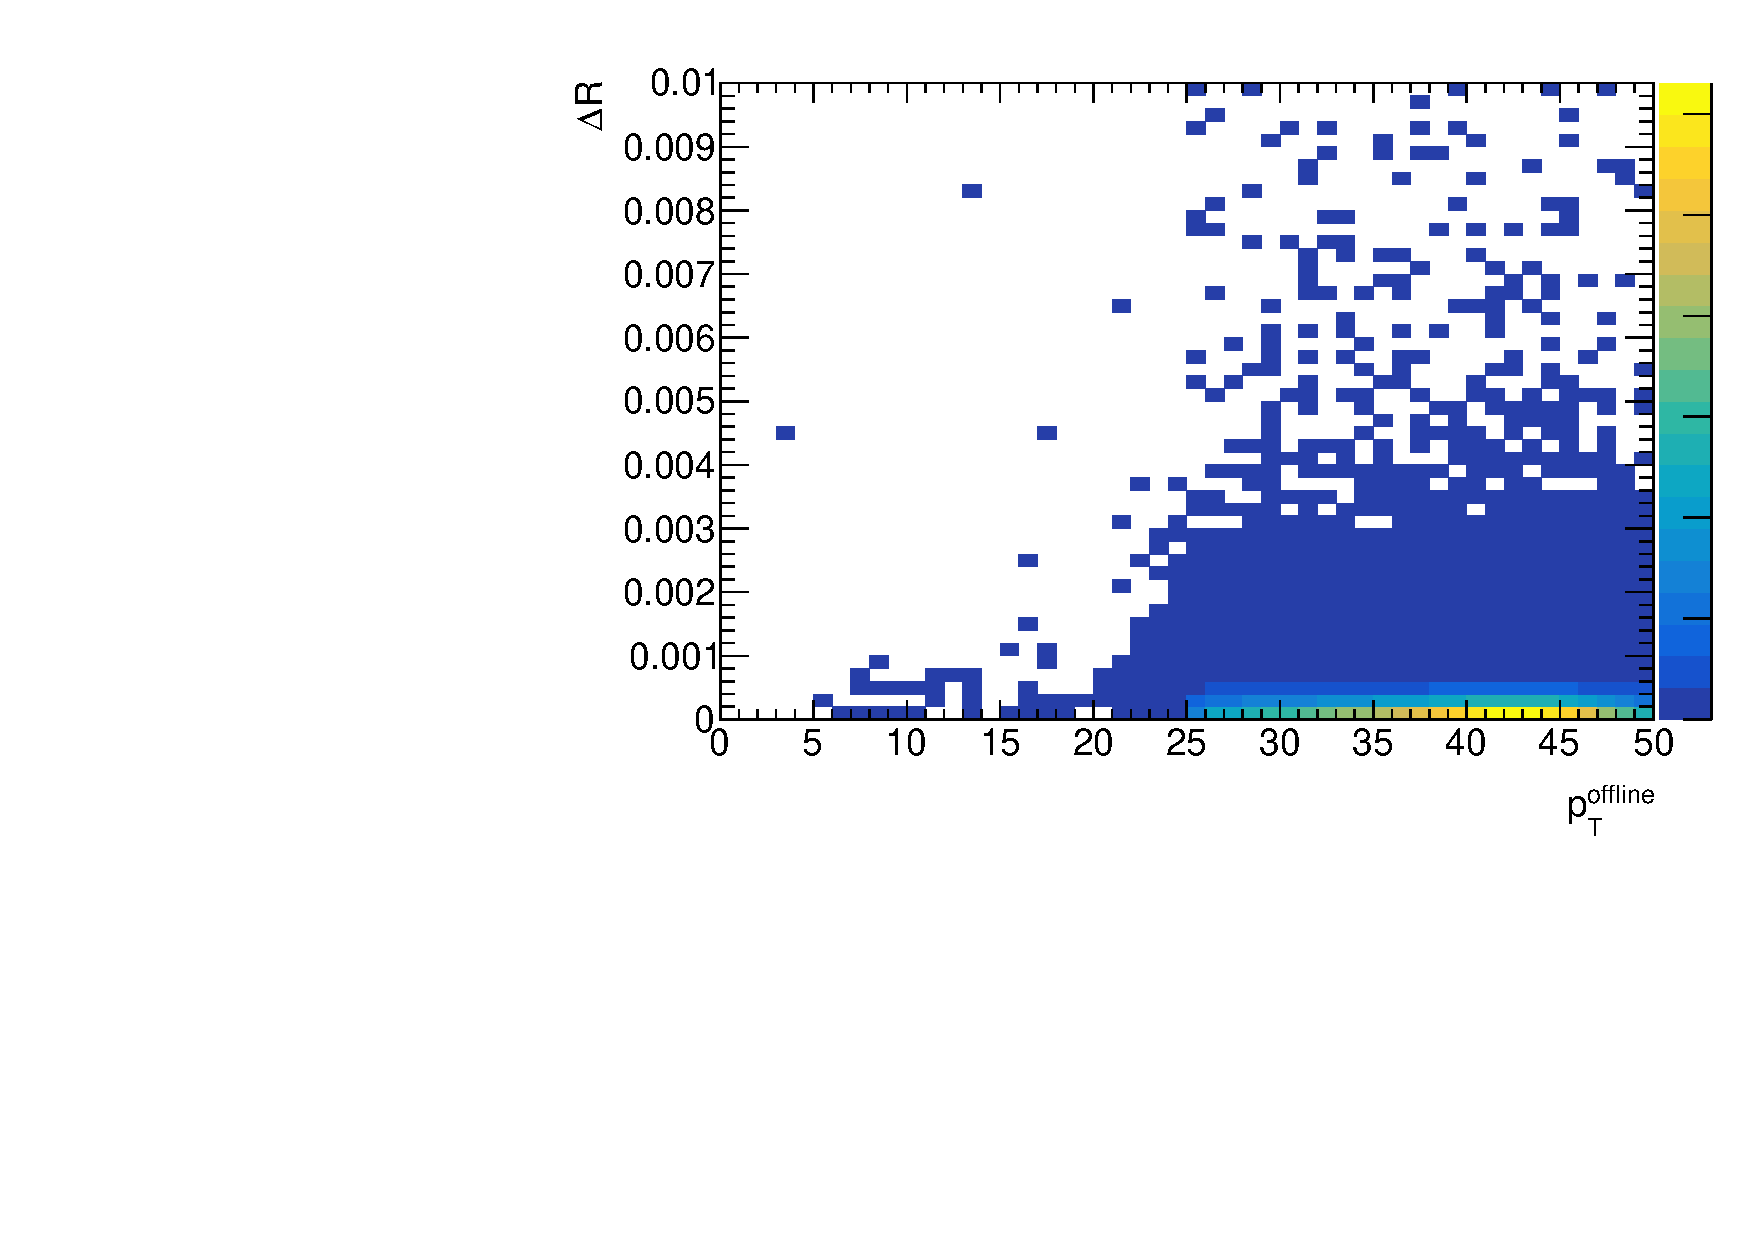
\includegraphics[clip, width=11cm]{fig/3/dR_tag_HLT.pdf}
  \caption{Tag ミューオンと HLT の $\Delta R$ 分布。$\Delta R < 0.001$ ならば Tag ミューオンが HLT を発行したものとする。}
  \label{fig:tag_HLT}
\end{figure}

Probe ミューオンは正しく再構成され、発行されたトリガーとは独立なミューオンである。
Probe ミューオンを使用してエンドキャプ部のトリガー性能を評価するために、Probe ミューオンと TGC のヒット情報を一致させる。図\ref{fig:Probe_TGC}に Probe ミューオンと TGC のヒット情報 の $\Delta R$ 分布を示す。本研究では$\Delta R < 0.04$ を満たせば Probe ミューオンが TGC のヒット情報と一致したものとする。
Probe ミューオンの情報とこのミューオンと一致したTGC のヒット情報を使って解析を行う。

\begin{figure}[tb]
  \centering
  %\rule{8cm}{6cm}
  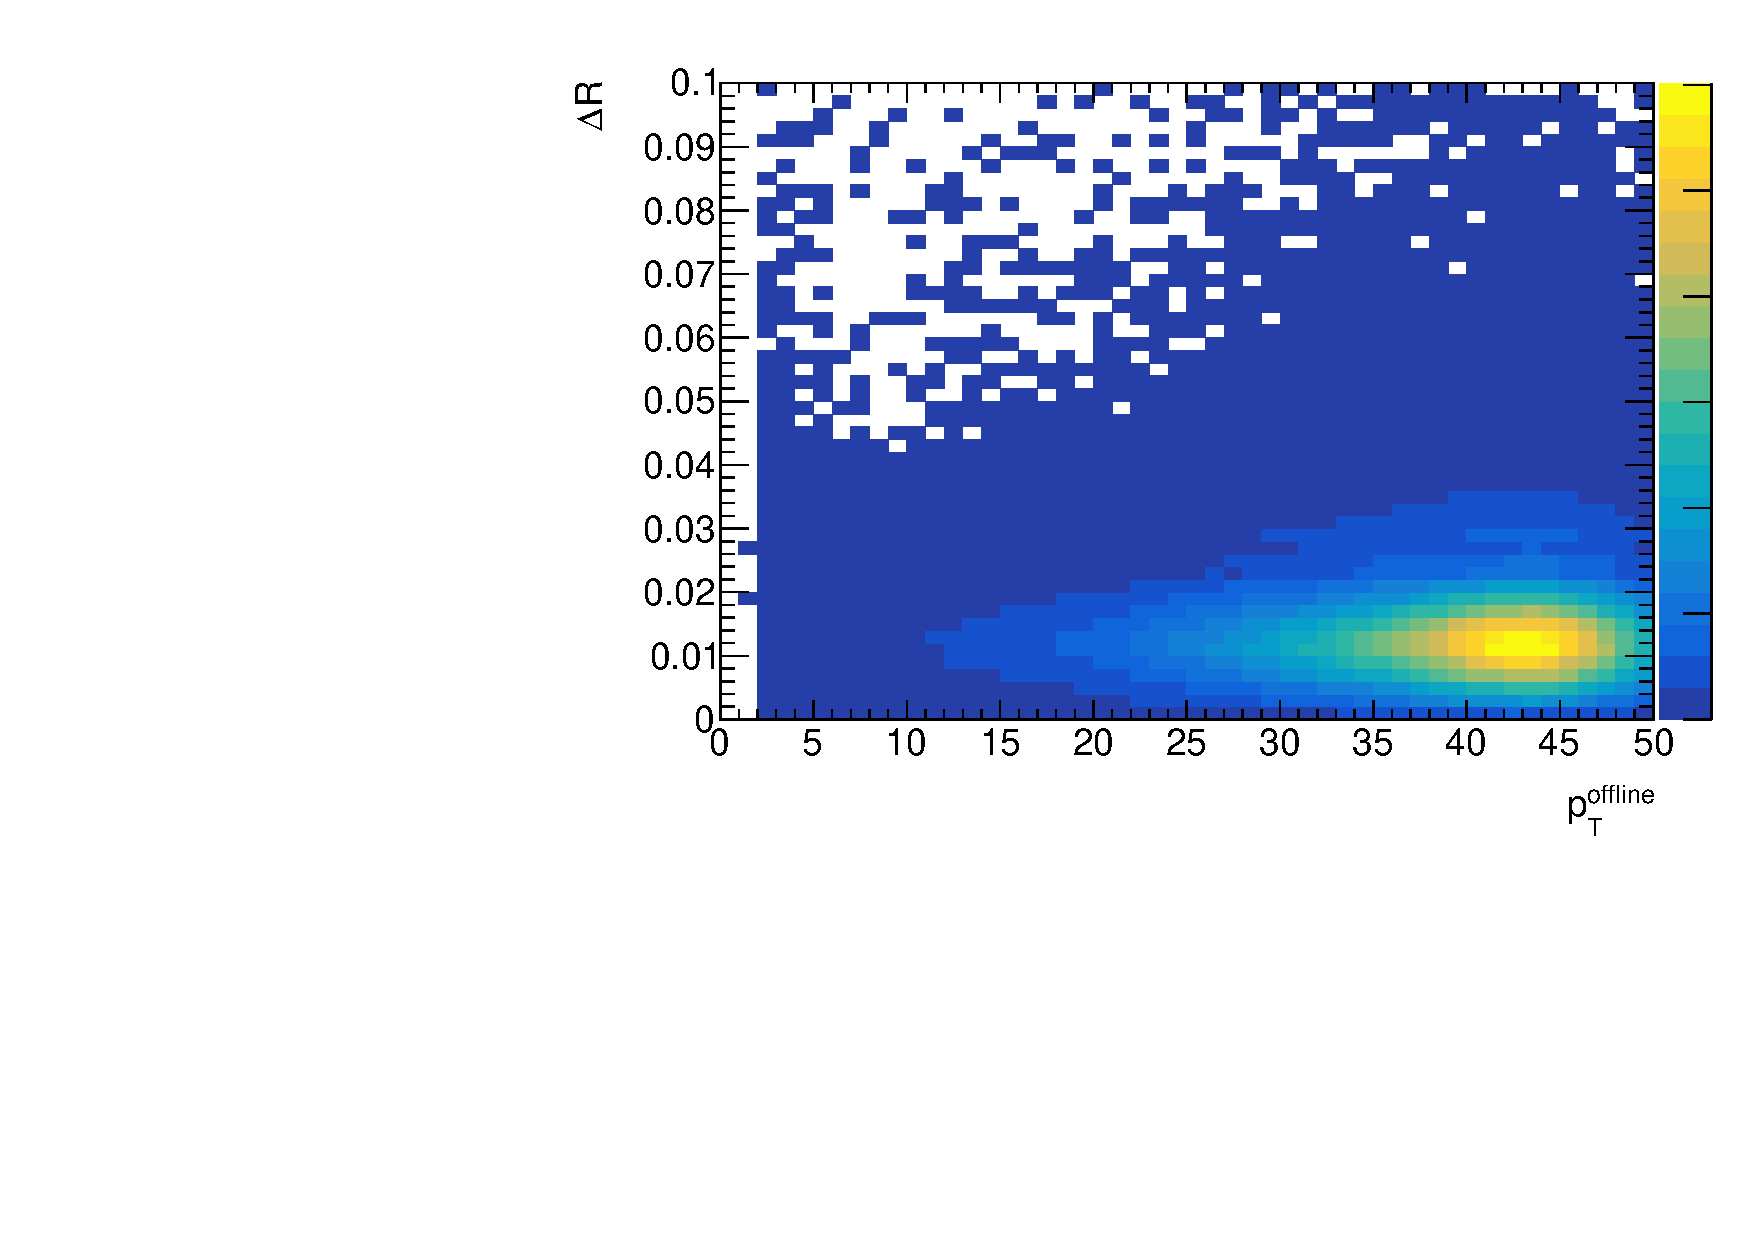
\includegraphics[clip, width=10cm]{fig/3/dR_probe_RoI.pdf}
  \caption{Probe ミューオンと TGC 1ヒット情報との $\Delta R$ 分布。$\Delta R < 0.04$ ならば Probe ミューオンが TGC のヒット情報と一致したものとする。}
  \label{fig:Probe_TGC}
\end{figure}



\subsection{トリガーの効率の算出}
トリガー効率$\epsilon$について式\ref{equ:Eff}を用いて評価を行う。
ここで、全ミューオン数はTGC にヒットした全オフラインミューオンと定義し、その中でトリガーを発行したミューオンの数を調べ、トリガー効率を計算する。
このとき得られるトリガー効率を $p_T$ の関数で表したプロットを Turn-on curve と呼ぶ。
\begin{equation}
 \epsilon=\frac{ある閾値のトリガーを発行したミューオンの数}{TGCにヒットした全ミューオンの数}
 \label{equ:Eff}
\end{equation}
シングルミューオンのシミュレーションサンプルに対してトリガー効率を計算し、2022年Run-3 で使用されているトリガーの各閾値における Turn-on curve を図\ref{fig:Run3_15_MC}に示す。
\begin{figure}[tb]
  \centering
  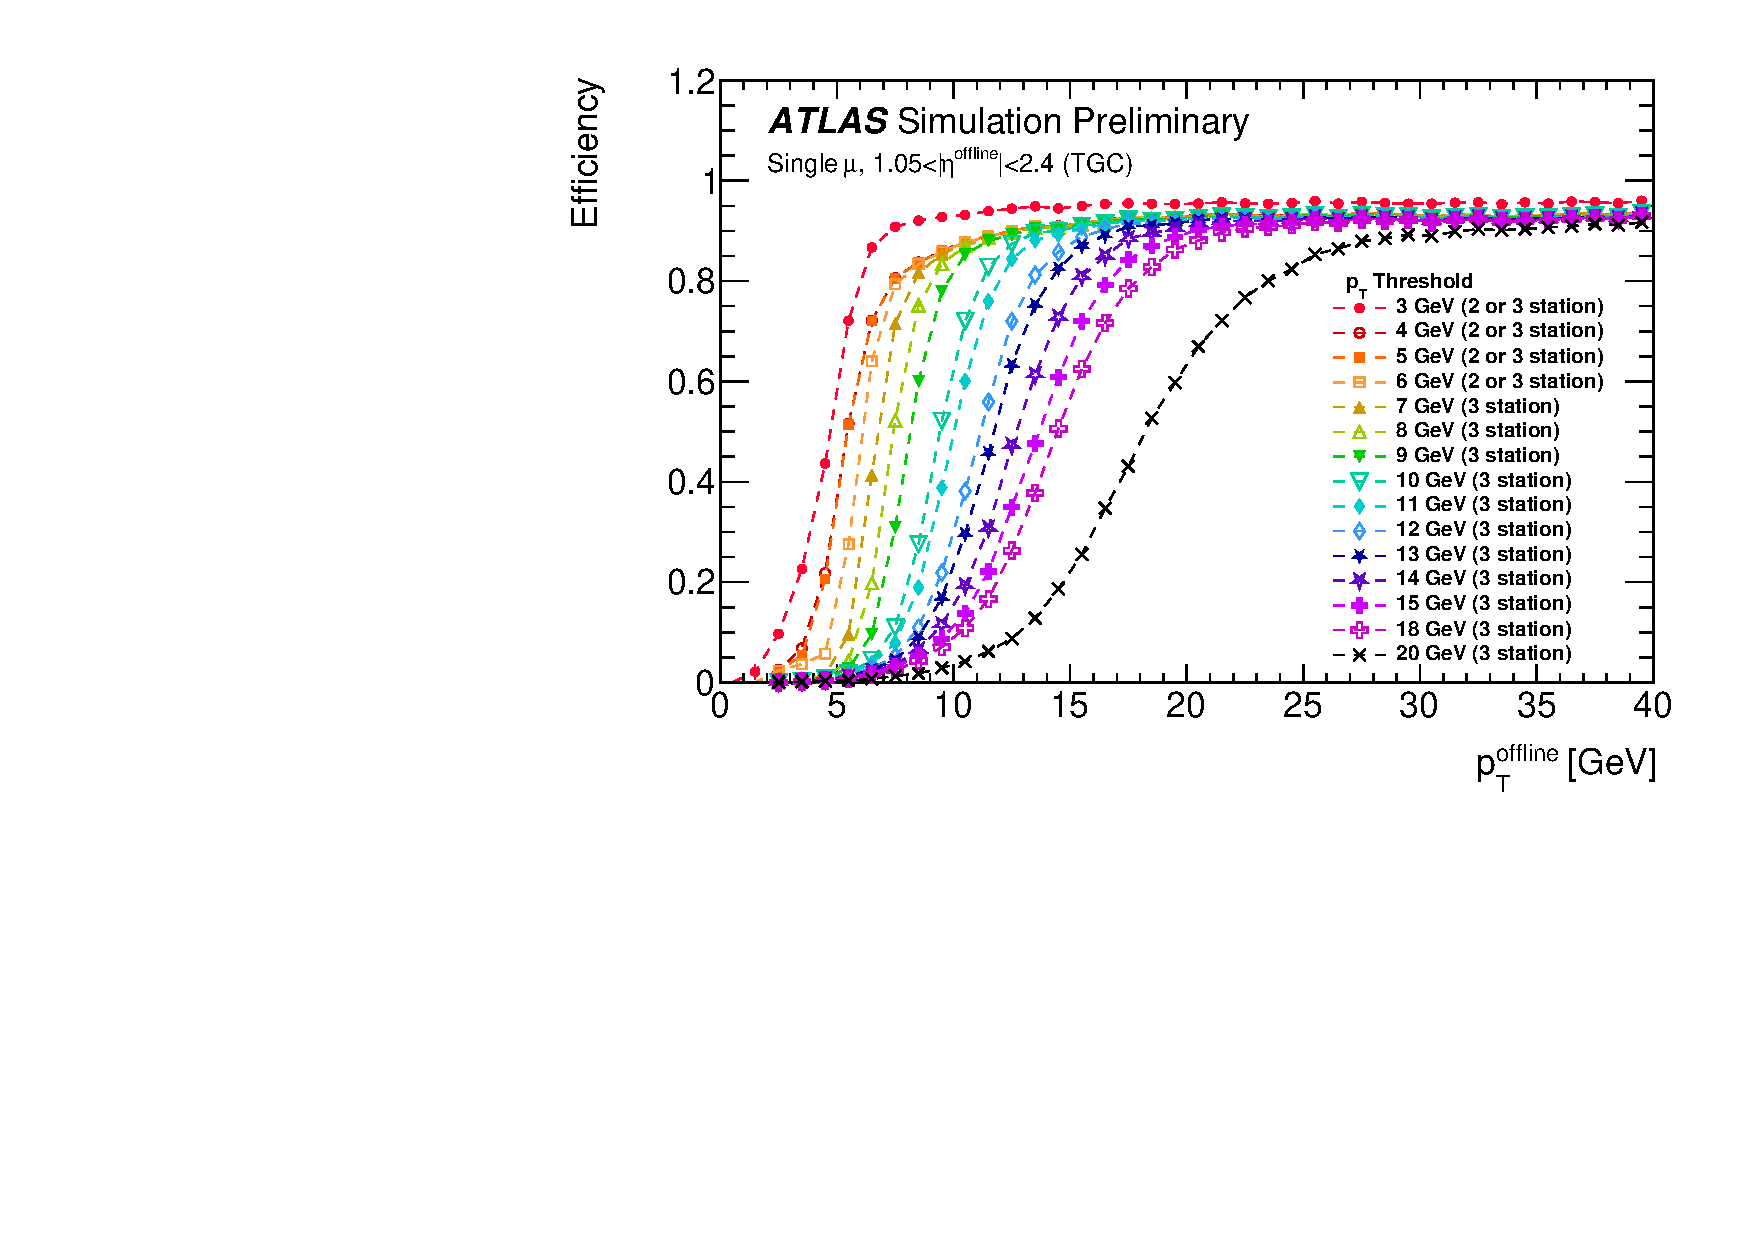
\includegraphics[clip, width=15cm]{fig/3/PLOT-TRIG-2020-01-fig1.pdf}
  \caption{Run-3 における15段階閾値のTurn-on curve。シングルミューオンのシミュレーションサンプルに対してのトリガー効率を示している。}
  \label{fig:Run3_15_MC}
\end{figure}
また、Run-3 の実データに対してトリガー効率を計算し、各閾値におけるトリガー効率を pT の関数として表した結果を図\ref{fig:Run3_15_Data}に示す。
\begin{figure}[tb]
  \centering
  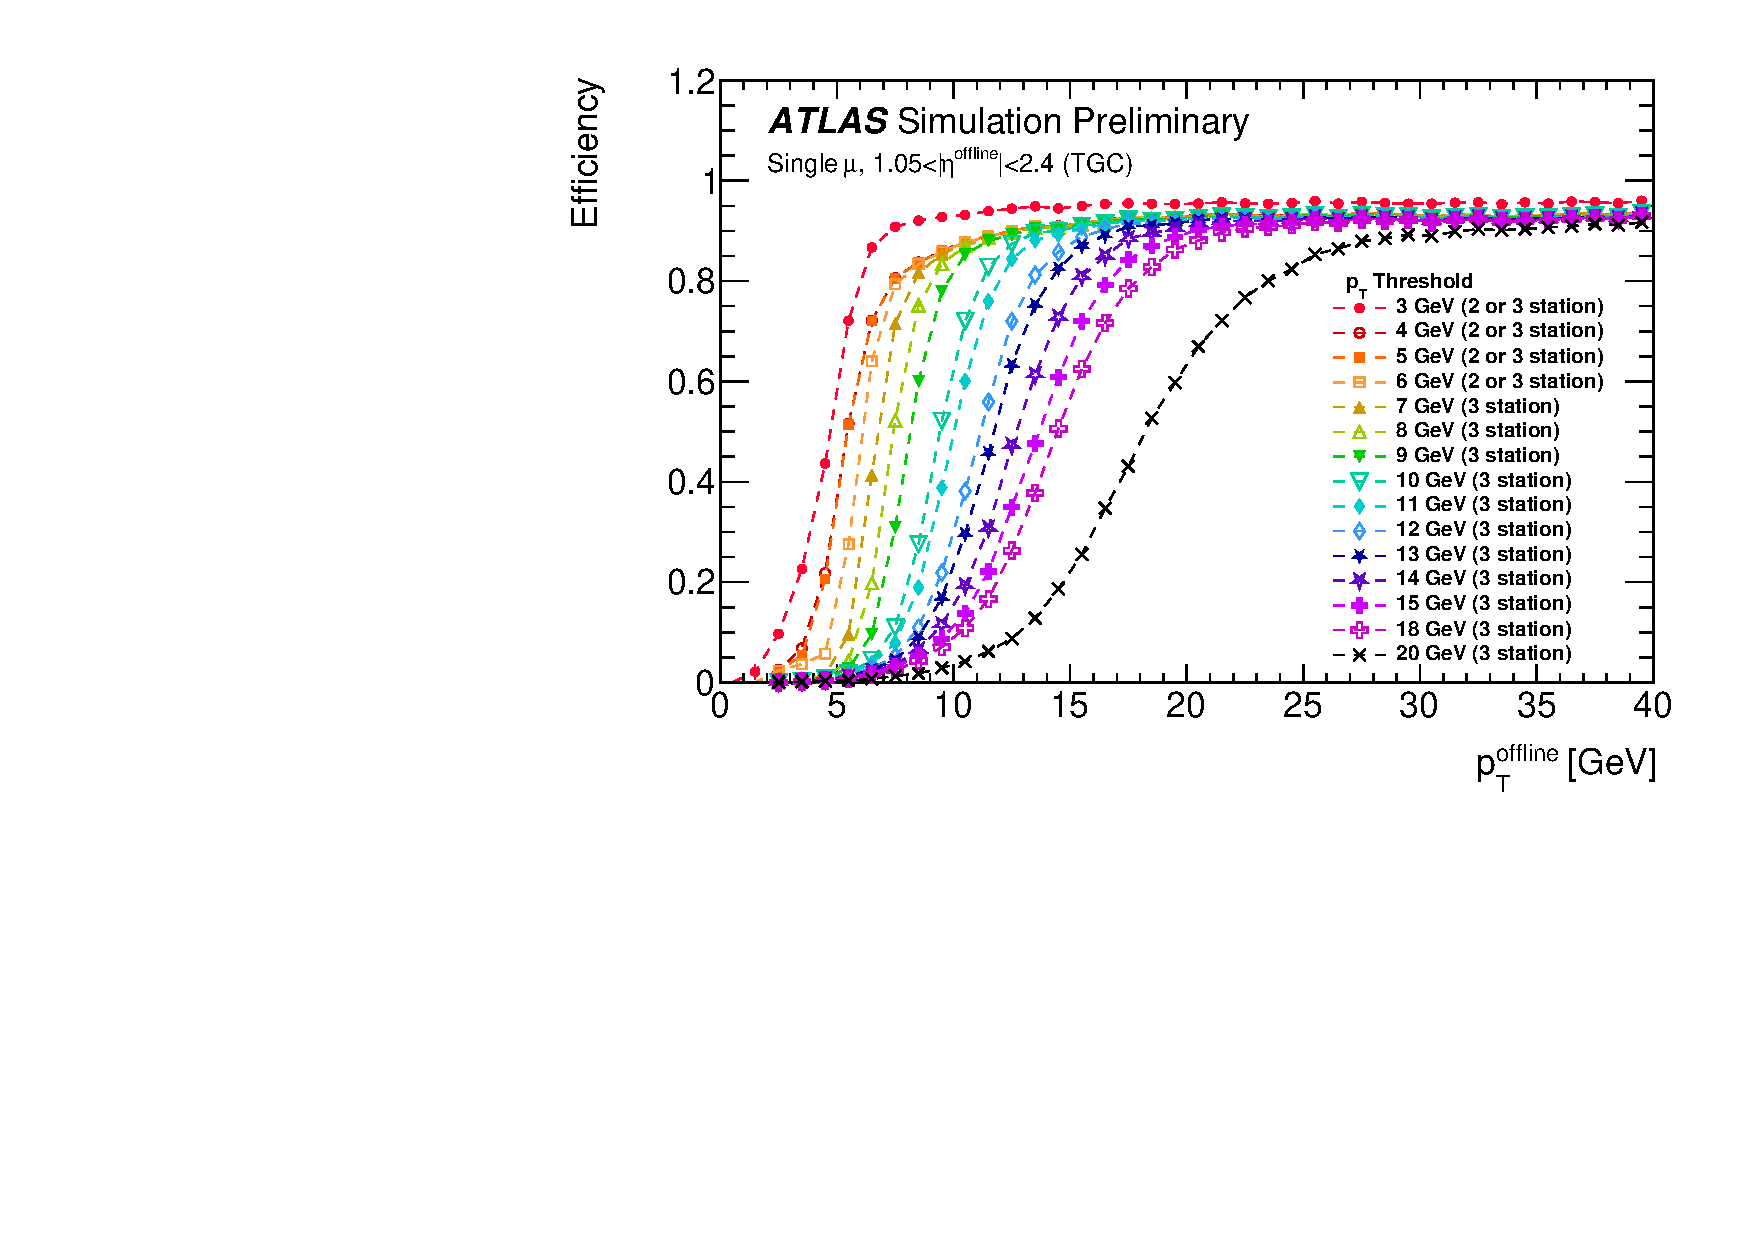
\includegraphics[clip, width=15cm]{fig/3/PLOT-TRIG-2020-01-fig1.pdf}
  \caption{Run-3 における15段階閾値のTurn-on curve。Run-3 の実データに対してのトリガー効率を示している。}
  \label{fig:Run3_15_Data}
\end{figure}

\subsection{トリガーレートの算出}
トリガーレートとは、実験データにおけるトリガーが発行された事象数である。ここでは HLT でのトリガー発行のバイアスを防ぐために、L1 Trigger のみを要求し、HLT は passthrough のトリガーである 「HLT$\_$noalg$\_$L1MU20」を要求する。 は 2016 年で取得されたデータを用いて算出したトリガーレートの $\eta$ 依存性である。

\begin{figure}[tb]
  \centering
  \rule{8cm}{6cm}
  \caption{Rate}
  \label{fig:Run3_rate}
\end{figure}



\subsection{CW の作成及び最適化手法}\label{section:最適化}
\subsection{15段階閾値に対応した Coincidence Window の作成手法}
Run-3 に向けた 15 段階の $p_T$ 閾値に対応した Coincidence Window (CW) は先行研究で作成されており、本節では先行研究で行われた作成手法について述べる。

シングルミューオンの MC サンプルを用いてミューオンの運動量と TGC におけるヒット位置の関係から CW を作成する。ミューオンの $p_T$ を用いて 1 GeV から 40 GeV まで 1 GeV 刻みに CW を作成し、その中から 15 段階の CW を選定し $p_T$ を決定する。




シミュレーションにおいて TGC は設計通りの位置に設置されているが、実際の検出器では、設置位置 (アライメント) にズレが生じている。CW はシミュレーションから作成するため、作成された CW には TGC の設置位置によるズレが考慮されていない。そのため、想定されていたミューオンの飛跡から外れてしまうため、 CW を用いた運動量判定に影響が出てしまい、トリガーの運動量分解能の低下を招く原因となる。さらに、背景事象によるトリガーレートの向上にも影響する。
また、ミューオンの電荷にも影響がある。

\begin{figure}[tb]
  \centering
  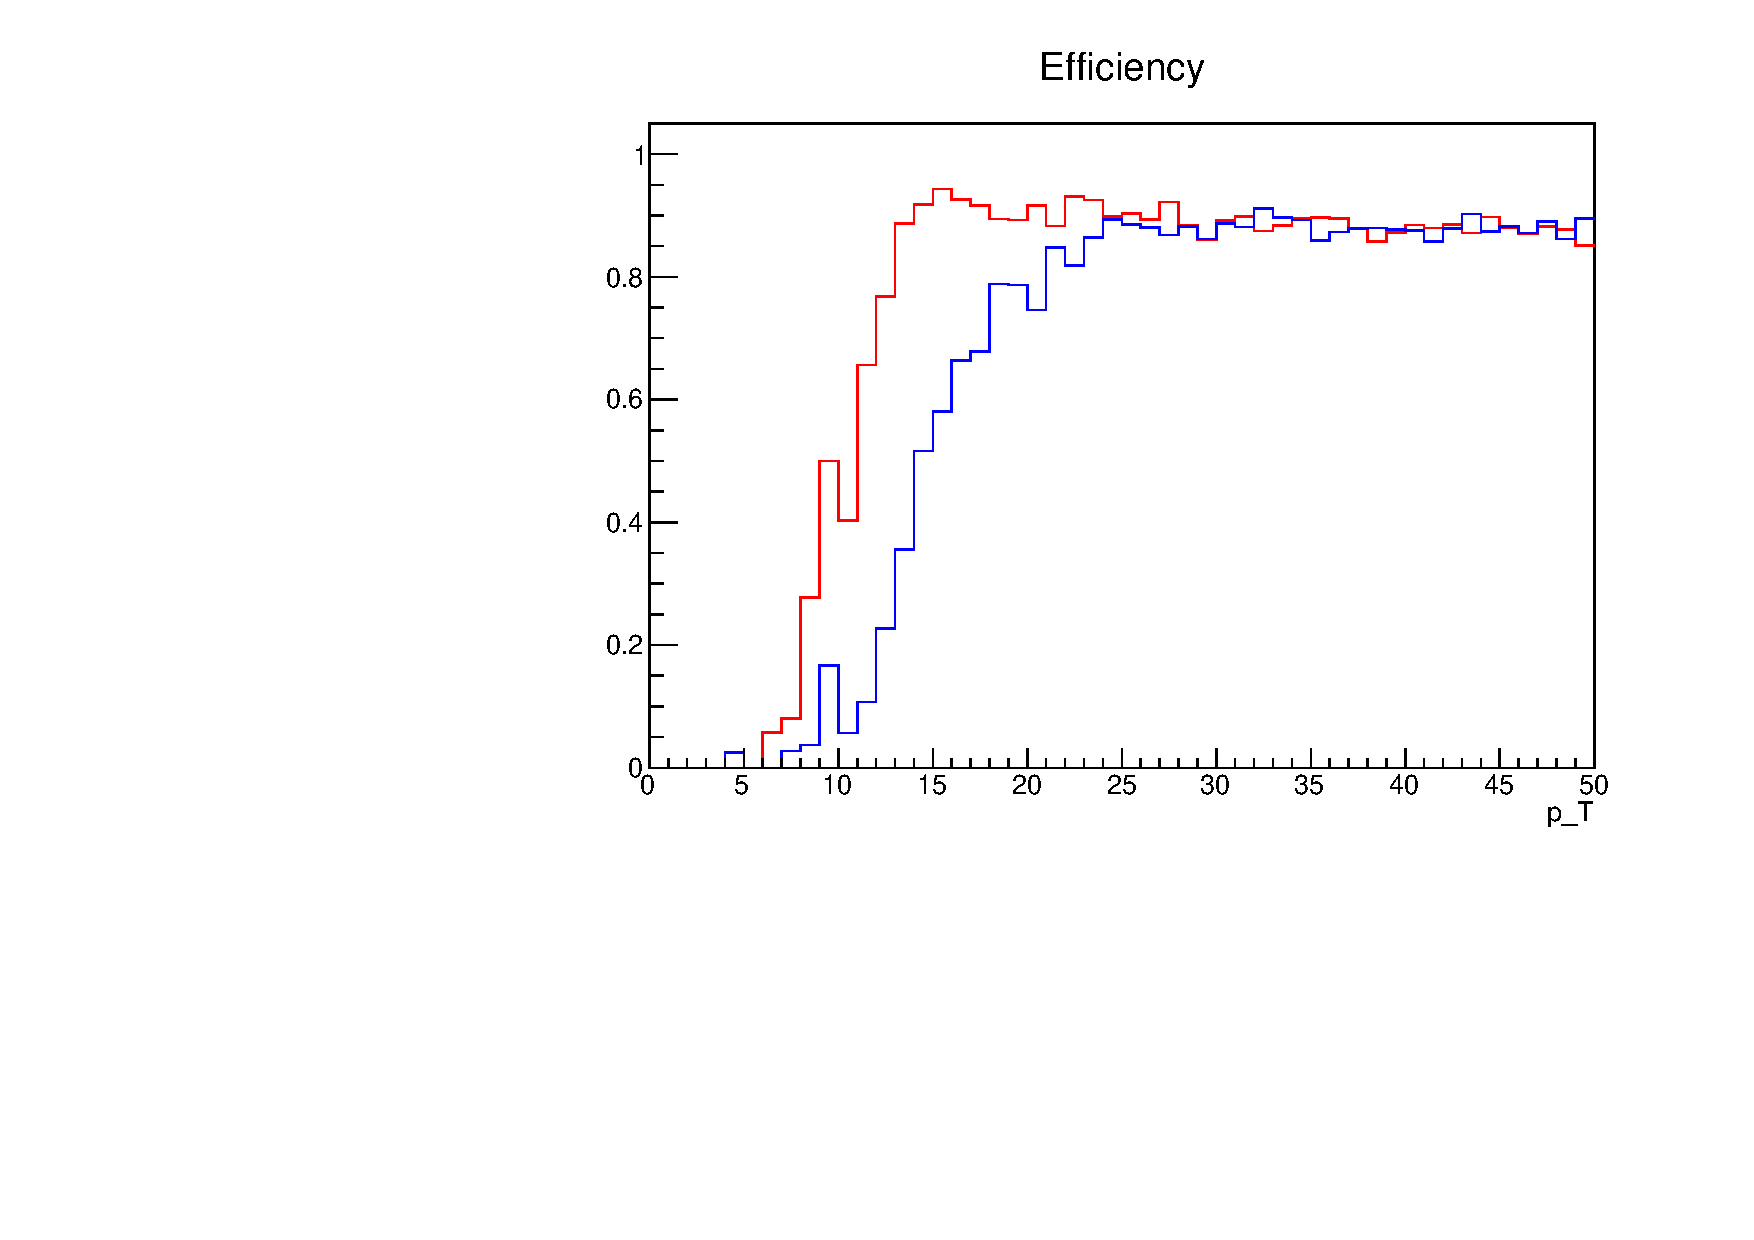
\includegraphics[clip, width=7cm]{fig/3/charge_14gev_phi2_eta11.pdf}
  \caption{あるチェンバーにおける電荷別のTurn-on curveの例。赤が正電荷、青が負電荷のTurn-on curveである。}
  \label{fig:fit_def}
\end{figure}

そこで、CW に対して検出器のズレを補正し最適化することで、トリガー効率を維持しつつ、トリガーレート削減を目指す。
以下では、これまでの研究で確立されている Run-2 で行われたTGC 検出器の設置位置のズレや歪みを考慮した CW の最適化の方法について述べる。

\subsection{TGC 検出器の設置位置の測定}
TGC 検出器は検出器の入れ替えなどのために検出器の移動を行うことがあり、検出器のズレが生じてしまう。TGC の設置位置のズレの測定方法はこれまでの研究で既に確立されている。
TGC 検出器のズレを示すパラメータを図\ref{fig:dr_para}のように定義し、図\ref{fig:ズレ}に Run-2 での実データを用いて測定した TGC 検出器の設置位置のズレを示す。
\begin{figure}[tb]
  \centering
  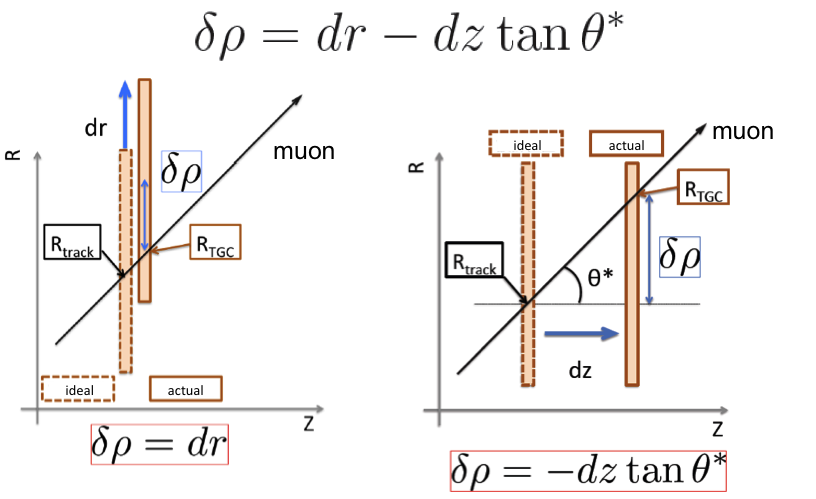
\includegraphics[clip, width=7cm]{fig/3/drho_param_position_measurement.png}
  \caption{TGC 検出器のズレを表すパラメータの定義。}
  \label{fig:dr_para}
\end{figure}

\begin{figure}
    %\begin{tabular}{cc}
    \begin{minipage}[tb]{0.4\linewidth}
        \centering
        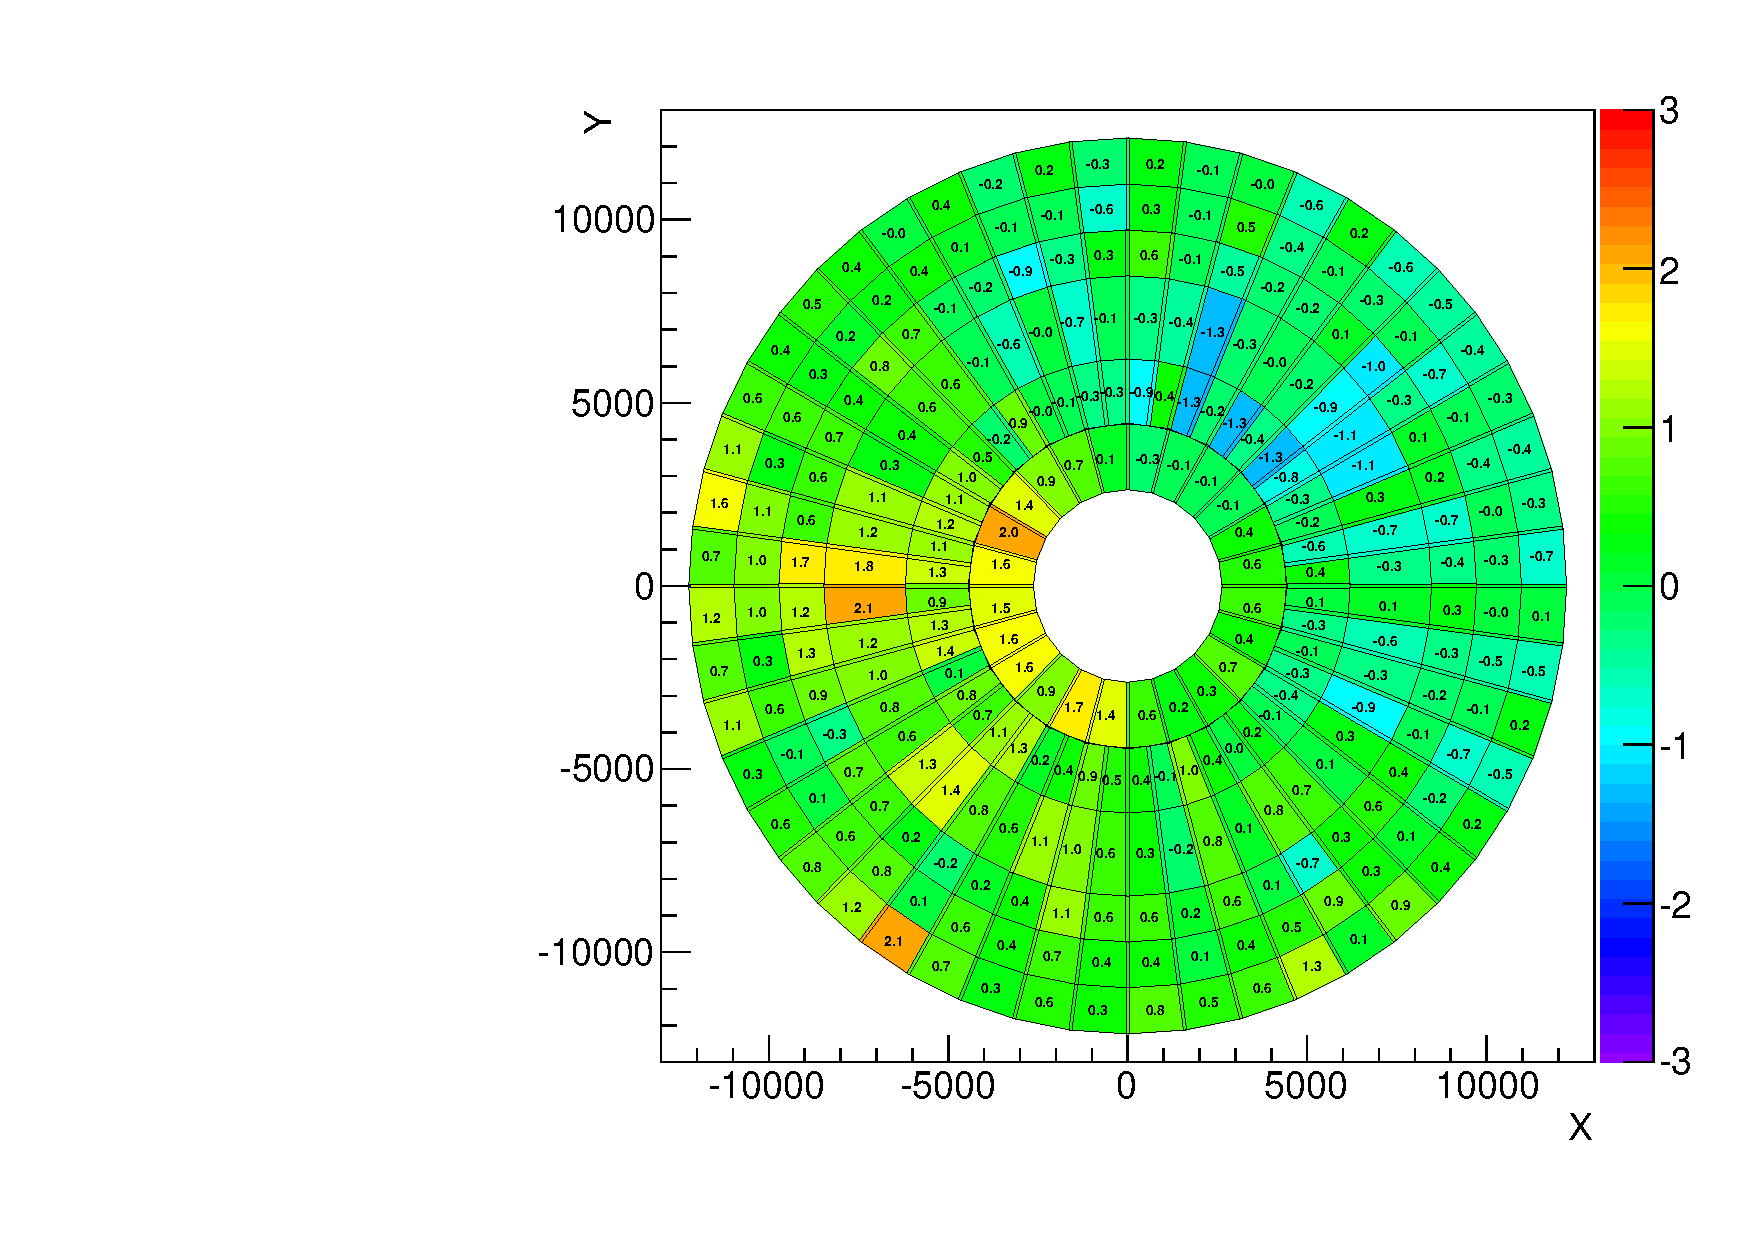
\includegraphics[clip, width=7cm]{fig/3/TGCAlign_CW.muon.bias.20160606.v1.A-side.pdf}
        \vspace{10pt}
        \subcaption{}
        \label{}
    \end{minipage}
    \hfill
    \begin{minipage}[tb]{0.4\linewidth}
        \centering
        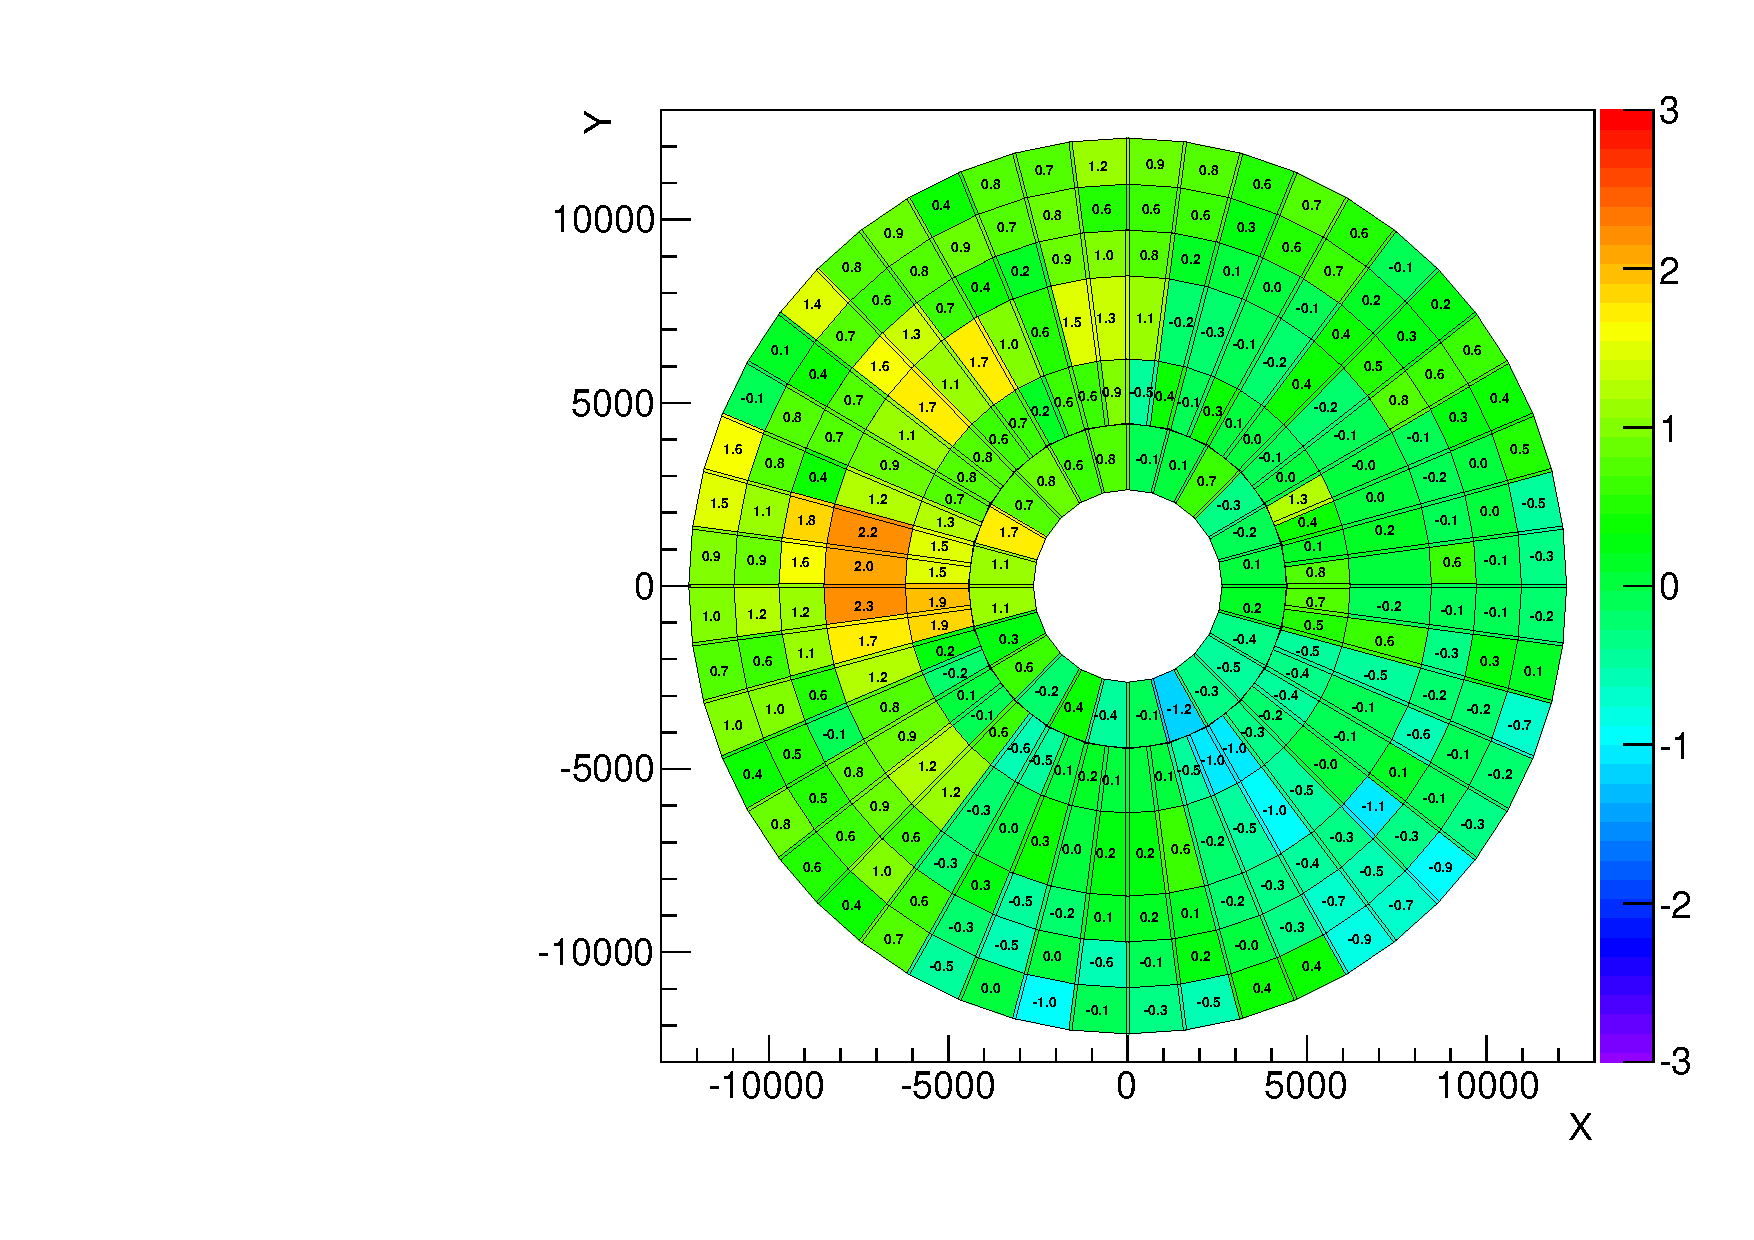
\includegraphics[clip, width=7cm]{fig/3/TGCAlign_CW.muon.bias.20160606.v1.C-side.pdf}
        \vspace{10pt}
        \subcaption{}
        \label{}
    \end{minipage}
    \caption{Run-2での検出器のズレの測定図。(a):A-side、(b):C-side}
    \label{fig:ズレ}
    %\end{tabular}
\end{figure}

\subsection{検出器アライメント}
Run-2 で行われたシミュレーションを用いて作成した CW に対する TGC のアライメントの補正方法について以下に述べる。

RoI 毎に pT 閾値を境目としたミューオン分布を用いた CW の cell 毎に判定するパラメータ $x$ を定義する。
\begin{equation}
    x = \frac{N_{p_{T}>20GeV}}{\sqrt{N^2_{p_{T}>20GeV}+N^2_{p_{T}<20GeV}}}
 \label{equ:fitting}
\end{equation}



\subsubsection{}
Run-2 では2015 年 Run-2 の実データを用いたこの CW を cell 毎に判定する方法を CW optimization と呼ぶ。


・検出器アライメント
<山内さんの手法>
<木戸さんの手法の説明>


\section{本研究の目的}
CW は事前にシミュレーションデータを用いたミューオンの運動量分布から統計的に作成する。そして、実際のデータをもとに、ある運動量を持つミューオンのヒットマップを作成し、ヒットマップと CW を比較することで検出器アライメントの補正値を判断して CW の最適化を行っている。
このように従来の CW の作成から最適化までの作業では、大量のシミュレーションデータや実際のデータの傾向を CW に反映させることを手動で行っていた。
そのため、Run-3における初段ミューオントリガーの性能を向上させるためには Run-2 と同様に CW の最適化を行う必要がある。しかし、\ref{section:最適化}節で述べたような Run-2 で行われていた最適化手法は、各CWごとに1マスずつ6段階の閾値を一段階ずつ確認する手法のため膨大な作業量が必要である。そのため、Run-3 で15段階に増設された閾値を持つ CW に対して Run-2 での最適化手法を行うことは現実的でない。
そこで、本研究では近年急速に発展している機械学習に着目し、新たな CW の最適化手法の開発を行う。
















\chapter{Run-3における近接2ミューオンのためのトリガーアルゴリズムの動作検証}\label{chapter5}

\section{Run-2までの2ミューオントリガーの非効率}\label{5-1}

\section{近接2ミューオントリガーアルゴリズム}\label{5-2}
2つのミューオン同士が近接している

\subsection{L1~BOMトリガー}
\subsection{L2mt}

\section{Run-3実データを用いた初段トリガーにおける近接2ミューオントリガーの動作検証}\label{5-3}

\section{Run-3実データを用いた後段トリガーにおける近接2ミューオントリガーの動作検証}\label{5-4}
\chapter{初段ミューオントリガーの性能評価}\label{chapter5}
本章では、第~\ref{chapter4}章で述べた手法を用いて作成した2種類のCW~(シミュレーション用のCWと実際の測定用のCW)を用いたトリガーの性能の評価を行う。

\section{機械学習を用いて作成したCWの15段階閾値の評価}
便宜上、本研究の手法で作成した2種類のCWについて、シミュレーション用のCWを$\mathrm{CW_{Simu}}$、実際の測定用のCWを$\mathrm{CW_{Data}}$と呼び、比較対象として2022年度Run-3で使用されたCWを$\mathrm{CW_{2022}}$と呼ぶこととする。

\ref{L1Topo}節で述べたL1トリガーには、ミューオンの不変質量を指針としたトリガーを持つL1Topoが存在する。しかし、不変質量を計算するときに使用するミューオンの運動量は、L1Muonから送られてくる$p_{\rm{T}}$閾値であるため、L1Muonの$p_{\rm{T}}$閾値の細かさがそのままL1Topoのトリガー性能に影響する。
そこで、Run-3ではL1Muonにおける判定可能な$p_{\rm{T}}$閾値を6段階から15段階に増設することで、より細かい精度での$p_{\rm{T}}$判定を可能とし、L1トリガー全体としてのトリガー性能の向上を図った。
したがって、本研究で作成するCWにも正確に15段階の$p_{\rm{T}}$判定ができることが要求される。

そこで、全オフライン再構成されたミューオンの内、ある$p_{\rm{T}}$閾値以上のトリガーが発行された割合$\epsilon$を計算し、トリガー効率の算出を行った。また、$\epsilon$をオフライン再構成した$p_{\rm{T}}$の関数として表したTurn-on curveを描き、式~\eqref{equ:fitting}の関数によってフィッティングを行う事で、トリガー性能の評価を行った。
このとき、Tag-And-Probe法を用いて評価に用いるデータの処理を行う。

\subsection{作成したCWの15段階の$p_{\rm{T}}$閾値}
図~\ref{fig:15Eff_CW_Data}に$\mathrm{CW_{Data}}$を用いて15段階の$p_{\rm{T}}$閾値におけるTurn-on curveを示す。評価には2018年Run-2 のデータに対して$Z\rightarrow \mu\mu$によるTag-And-Probe法を用いた。
$\mathrm{CW_{2022}}$と同様に、本研究の手法で作成した$\mathrm{CW_{Data}}$は15段階に分かれたTurn-on curveを描けていることがわかる。
また、図~\ref{fig:15Eff_CW_Simu}に$\mathrm{CW_{Simu}}$を用いてを要求した15段階の$p_{\rm{T}}$閾値におけるTurn-on curveを示す。評価にはシングルミューオンのシミュレーションサンプルを用いた。
比較のため、図~\ref{fig:Run3_15_MC5} に $\mathrm{CW_{2022}}$を用いた15段階の$p_{\rm{T}}$閾値におけるのTurn-on curveを示す。
こちらも同様に、本研究の手法で作成した$\mathrm{CW_{Simu}}$は15段階に分かれたTurn-on curveを描けていることがわかる。
よって、本研究の手法によって作成された2種類のCWは、2022年度Run-3において使用された$\mathrm{CW_{2022}}$と同様に細かい精度で15段階の判定が可能であることが見て取れる。
ここから、本研究の手法を用いて、15段階の閾値を持ったCWの作成が可能であることが確認できる。
\begin{figure}
    %\centering
    \begin{tabular}{cc}
    \begin{minipage}[b]{0.45\hsize}
        %\centering
        \hspace*{-1cm}
        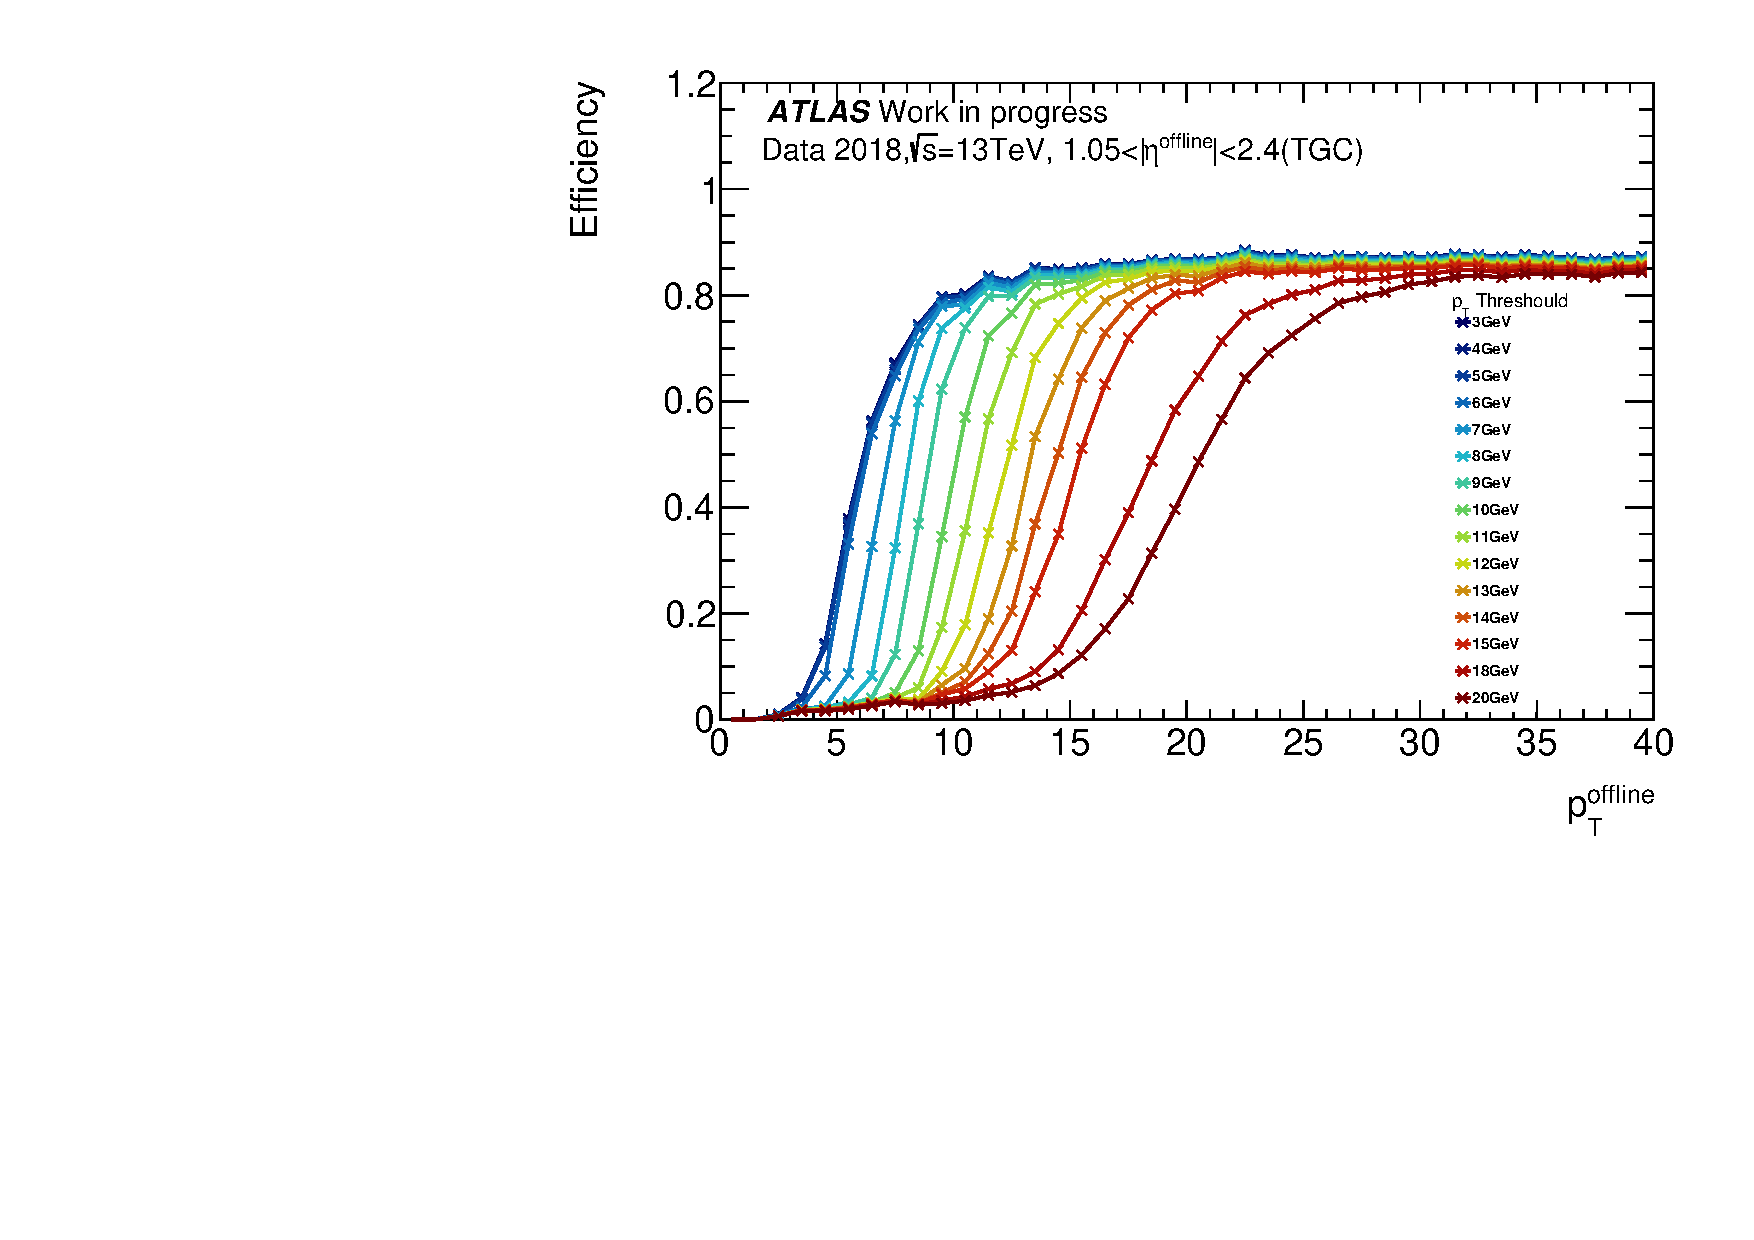
\includegraphics[clip, width=8cm]{fig/5/15_v06_Data.pdf}
        %\vspace{5pt}
        \subcaption{$\mathrm{CW_{Data}}$のTurn-on curve}
        \label{fig:15Eff_CW_Data}
    \end{minipage}&
    %\hfill
    \begin{minipage}[b]{0.55\hsize}
        %\centering
        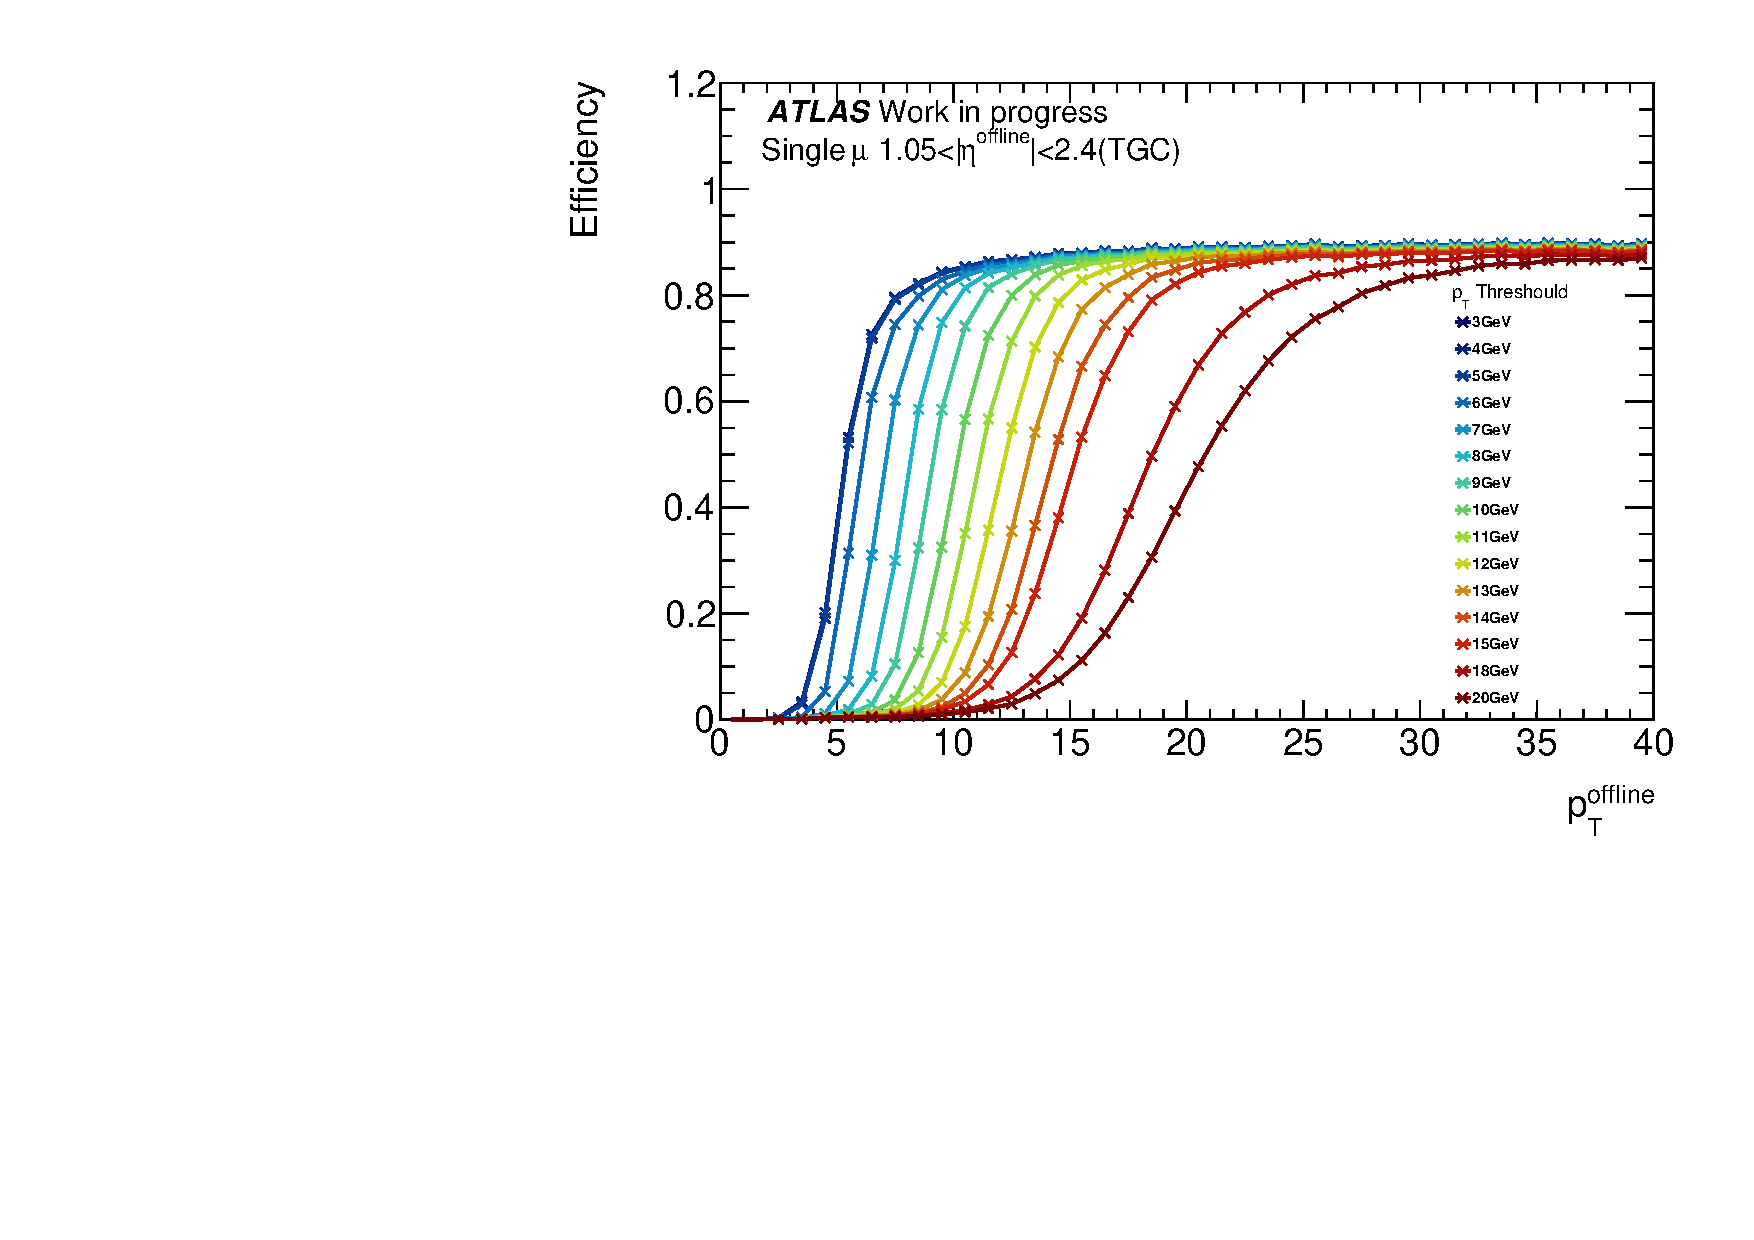
\includegraphics[clip, width=8cm]{fig/5/15_MC_MC.pdf}
        %\vspace{5pt}
        \subcaption{$\mathrm{CW_{Simu}}$のTurn-on curve}
        \label{fig:15Eff_CW_Simu}
    \end{minipage}
    \end{tabular}
    \caption{機械学習を用いて作成したCWの15段階の閾値におけるTurn-on curve。}
    \label{}
\end{figure}


\subsection{現行のトリガーとのトリガー性能の比較}
次に、それぞれの15段階の$p_{\rm{T}}$閾値のトリガー性能について評価を行う。

\subsubsection{トリガー効率の評価}
まず、$\mathrm{CW_{Simu}}$と$\mathrm{CW_{2022}}$の比較と、$\mathrm{CW_{Data}}$と$\mathrm{CW_{2022}}$の比較を行う。それぞれの評価には、シングルミューオンのシミュレーションデータと2018年Run-2のデータを評価に用いる。
ここでは、トリガー効率$\epsilon$を用いて比較を行う。

図~\ref{fig:v05v07}には$p_{\rm{T}}$閾値が14~GeVの時の、$\mathrm{CW_{2022}}$と$\mathrm{CW_{Simu}}$のTurn-on curveの比較を示し、図~\ref{fig:v05v06}には$p_{\rm{T}}$閾値が14~GeVの時の、$\mathrm{CW_{Data}}$を$\mathrm{CW_{2022}}$のTurn-on curveの比較を示す。

2022年度Run-3で使用されている$\mathrm{CW_{2022}}$に比べて、本研究の手法ので作成したCWの方がTurn-on curveの立ち上がりが鋭くなっており、トリガー性能が良くなっていることが見て取れる。
このとき、$\mathrm{CW_{2022}}$はトリガー効率が85.4$\%$であったのに対し、$\mathrm{CW_{Data}}$ではトリガー効率が86.7$\%$となったことから、約1$\%$の向上が確認できた。
また、図~\ref{fig:v05v07_1_9_Simu}と図~\ref{fig:v05v06_1_9_Data}に他の$p_{\rm{T}}$閾値における比較を示す。
15段階の閾値において、本研究の手法によって作成された2種類のCWは、2022年度Run-3において使用された$\mathrm{CW_{2022}}$と同様に鋭く立ち上がっていることが見て取れる。
\begin{figure}
    %\centering
    \begin{tabular}{cc}
    \centering
    \begin{minipage}[b]{0.45\hsize}%
        \centering
        \hspace*{-1.5cm}
        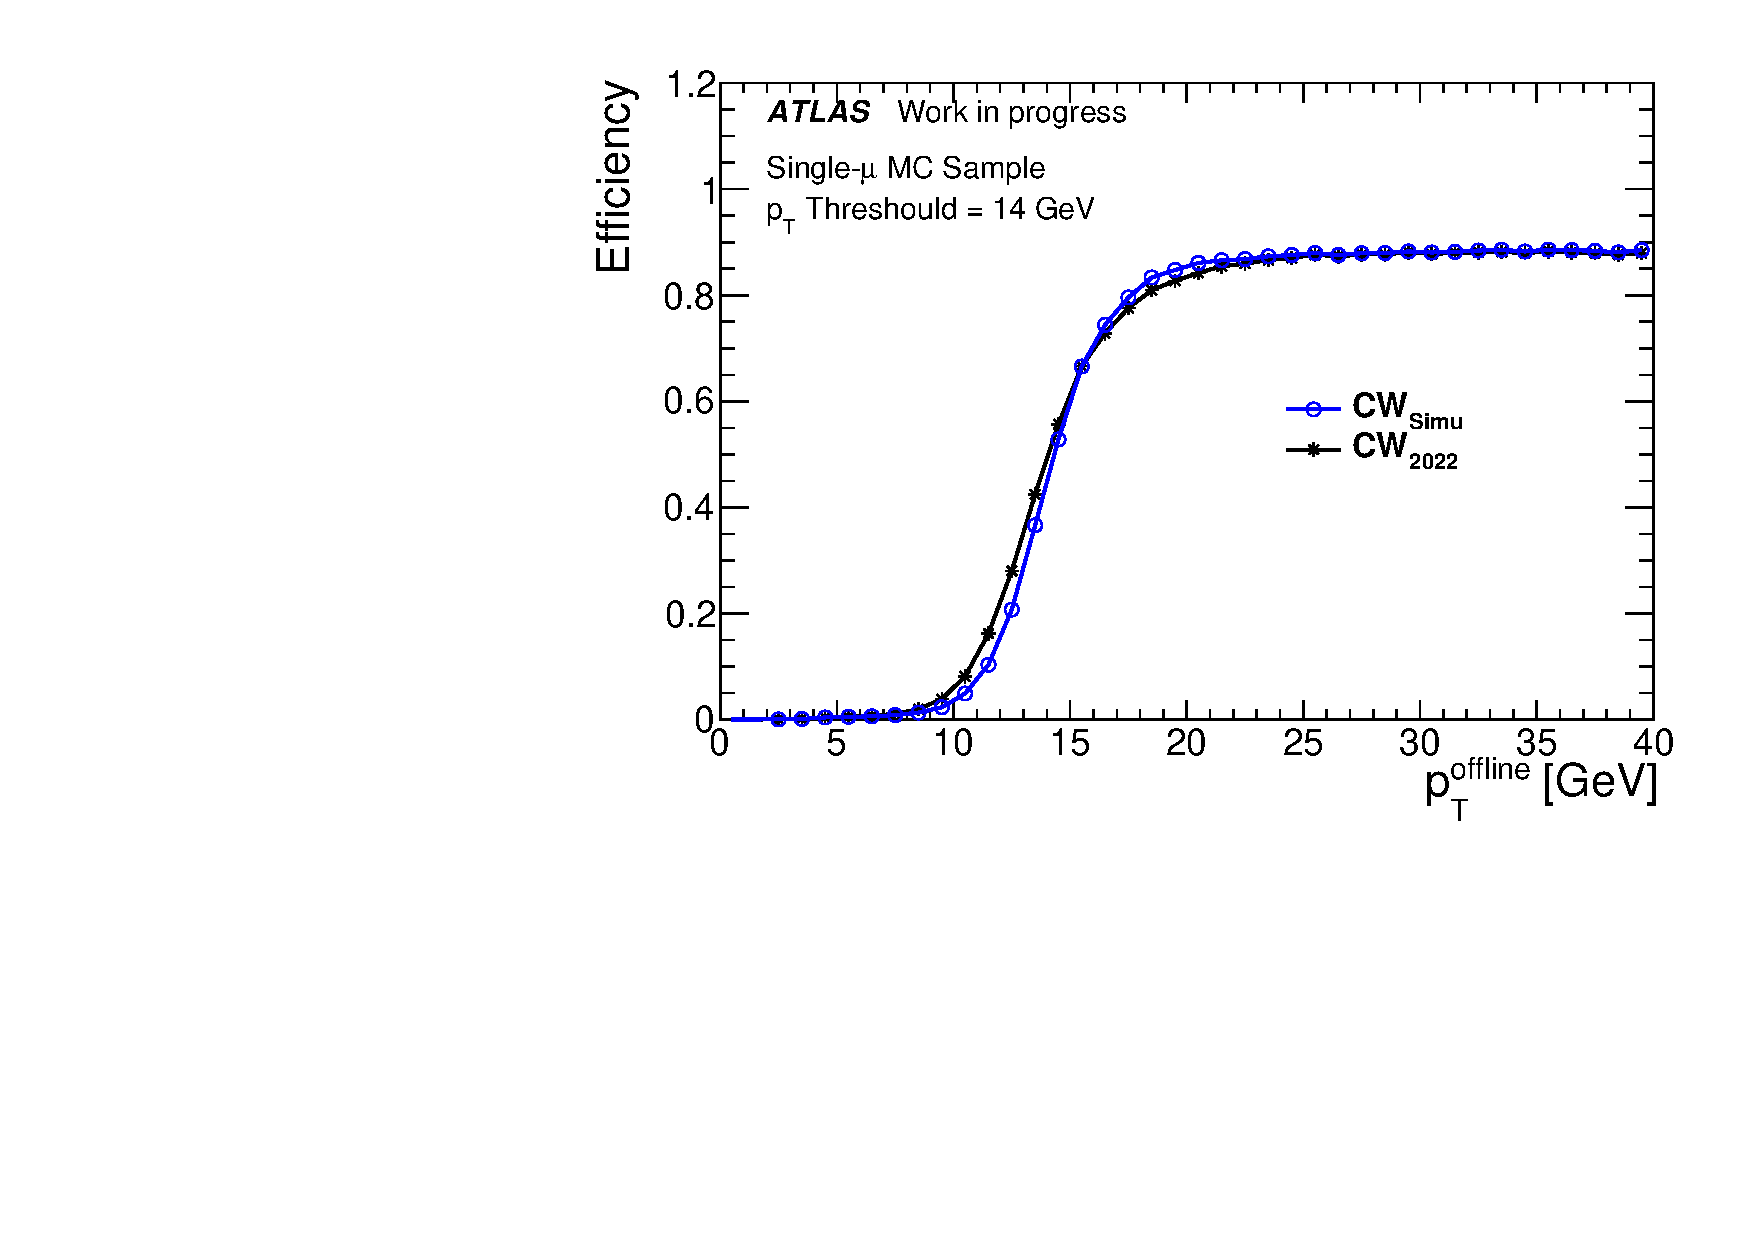
\includegraphics[clip, width=8cm]{fig/5/v05vsv07_MU14_re2.pdf}
        %\vspace{5pt}
        \subcaption{$\mathrm{CW_{Simu}}$と$\mathrm{CW_{2022}}$の比較。}
        \label{fig:v05v07}
    \end{minipage}%
    %\hfill
    \begin{minipage}[b]{0.7\hsize}%
        \centering
        \hspace*{-0.75cm}
        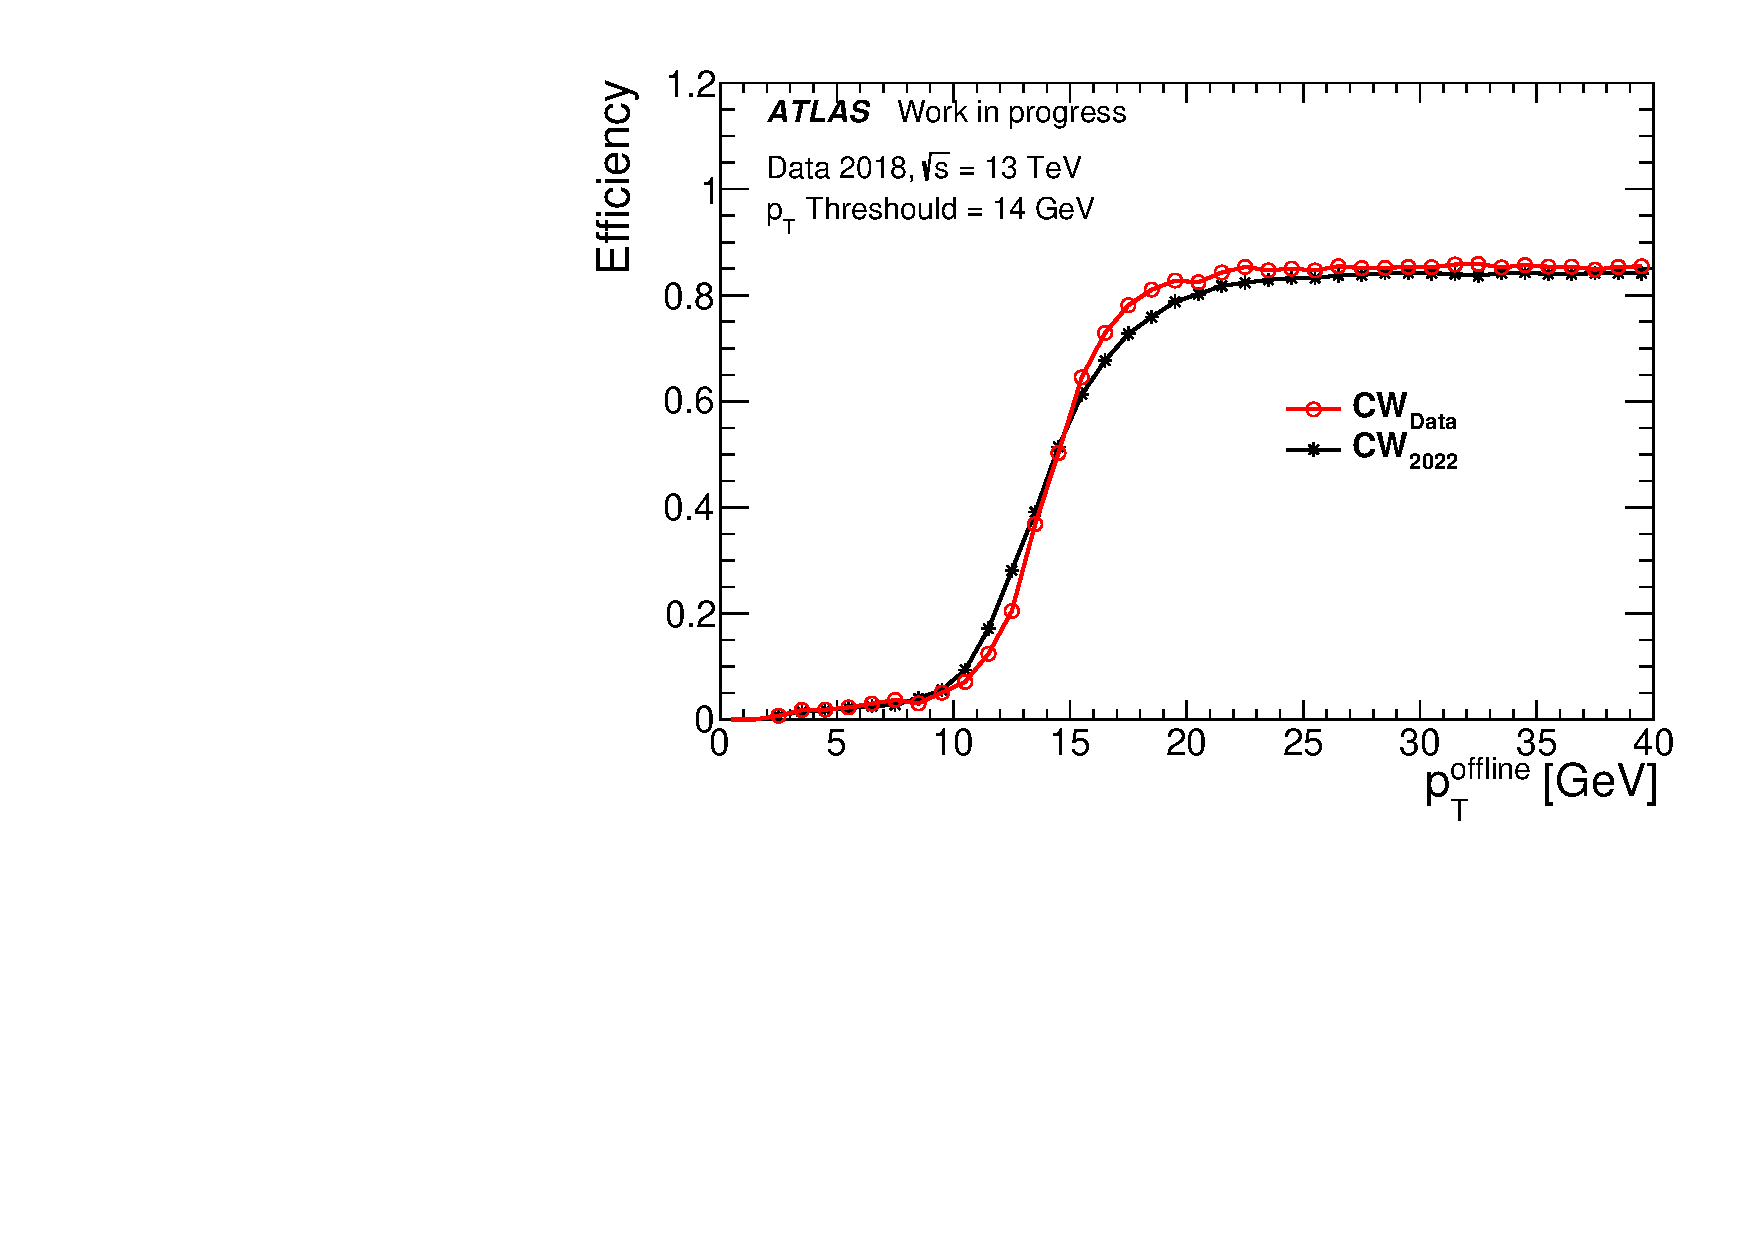
\includegraphics[clip, width=8cm]{fig/5/v05vsv06_MU14_re.pdf}
        %\vspace{5pt}
        \subcaption{$\mathrm{CW_{Data}}$と$\mathrm{CW_{2022}}$の比較。}
        \label{fig:v05v06}
    \end{minipage}%
    \end{tabular}
    \caption{$p_{\rm{T}}$閾値14~GeVにおけるTurn-on curveの比較。}
    \label{fig:v05v07v06}
\end{figure}

\begin{figure}[p]
  \centering
  %\rule{8cm}{6cm}
  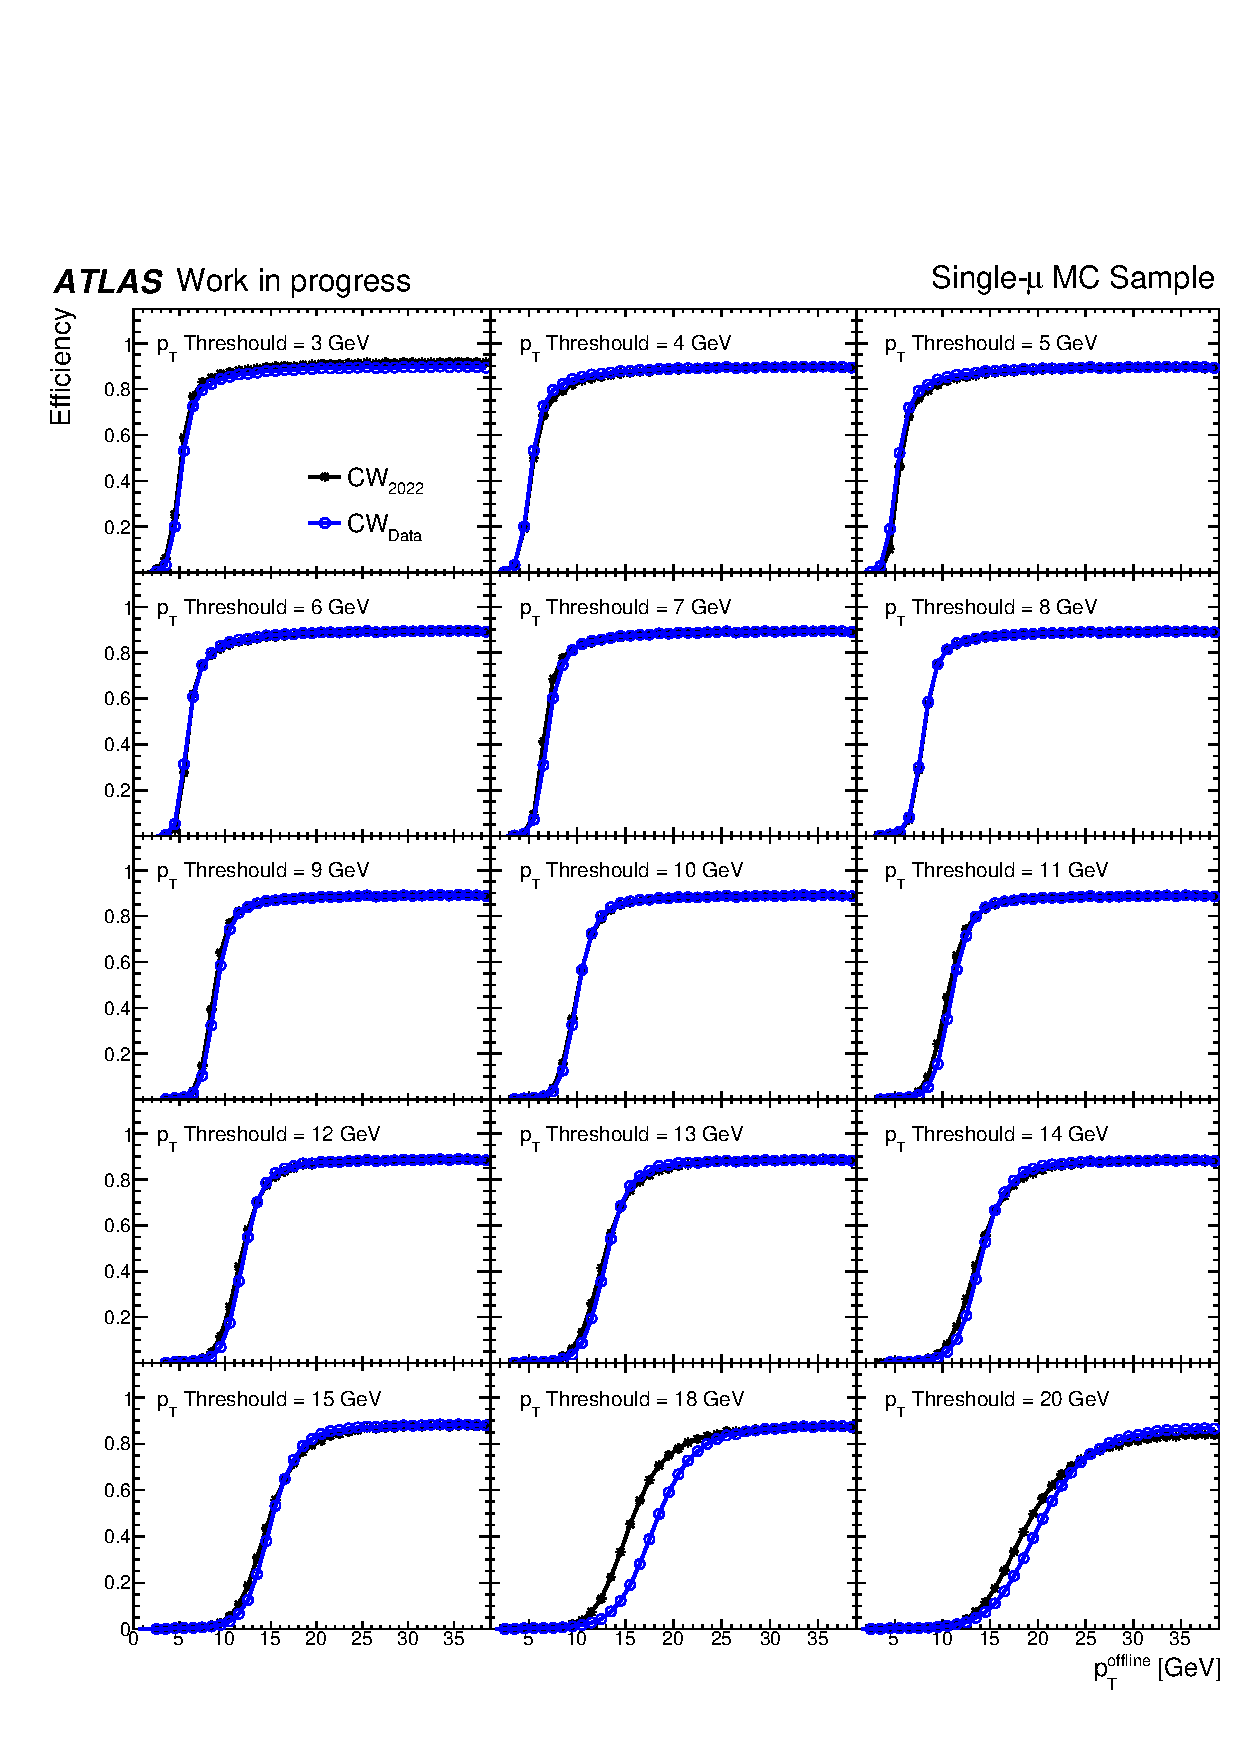
\includegraphics[clip, width=14cm]{fig/5/c2.pdf}
  \caption{$p_{\rm{T}}$閾値3~GeV$\sim$20~GeVにおける$\mathrm{CW_{Simu}}$と$\mathrm{CW_{2022}}$のTurn-on curveの比較。評価にはシングルミューオンのシミュレーションデータを使用した。}
  \label{fig:v05v07_1_9_Simu}
\end{figure}


%\begin{figure}[htb]
%  \centering
%  %\rule{8cm}{6cm}
%  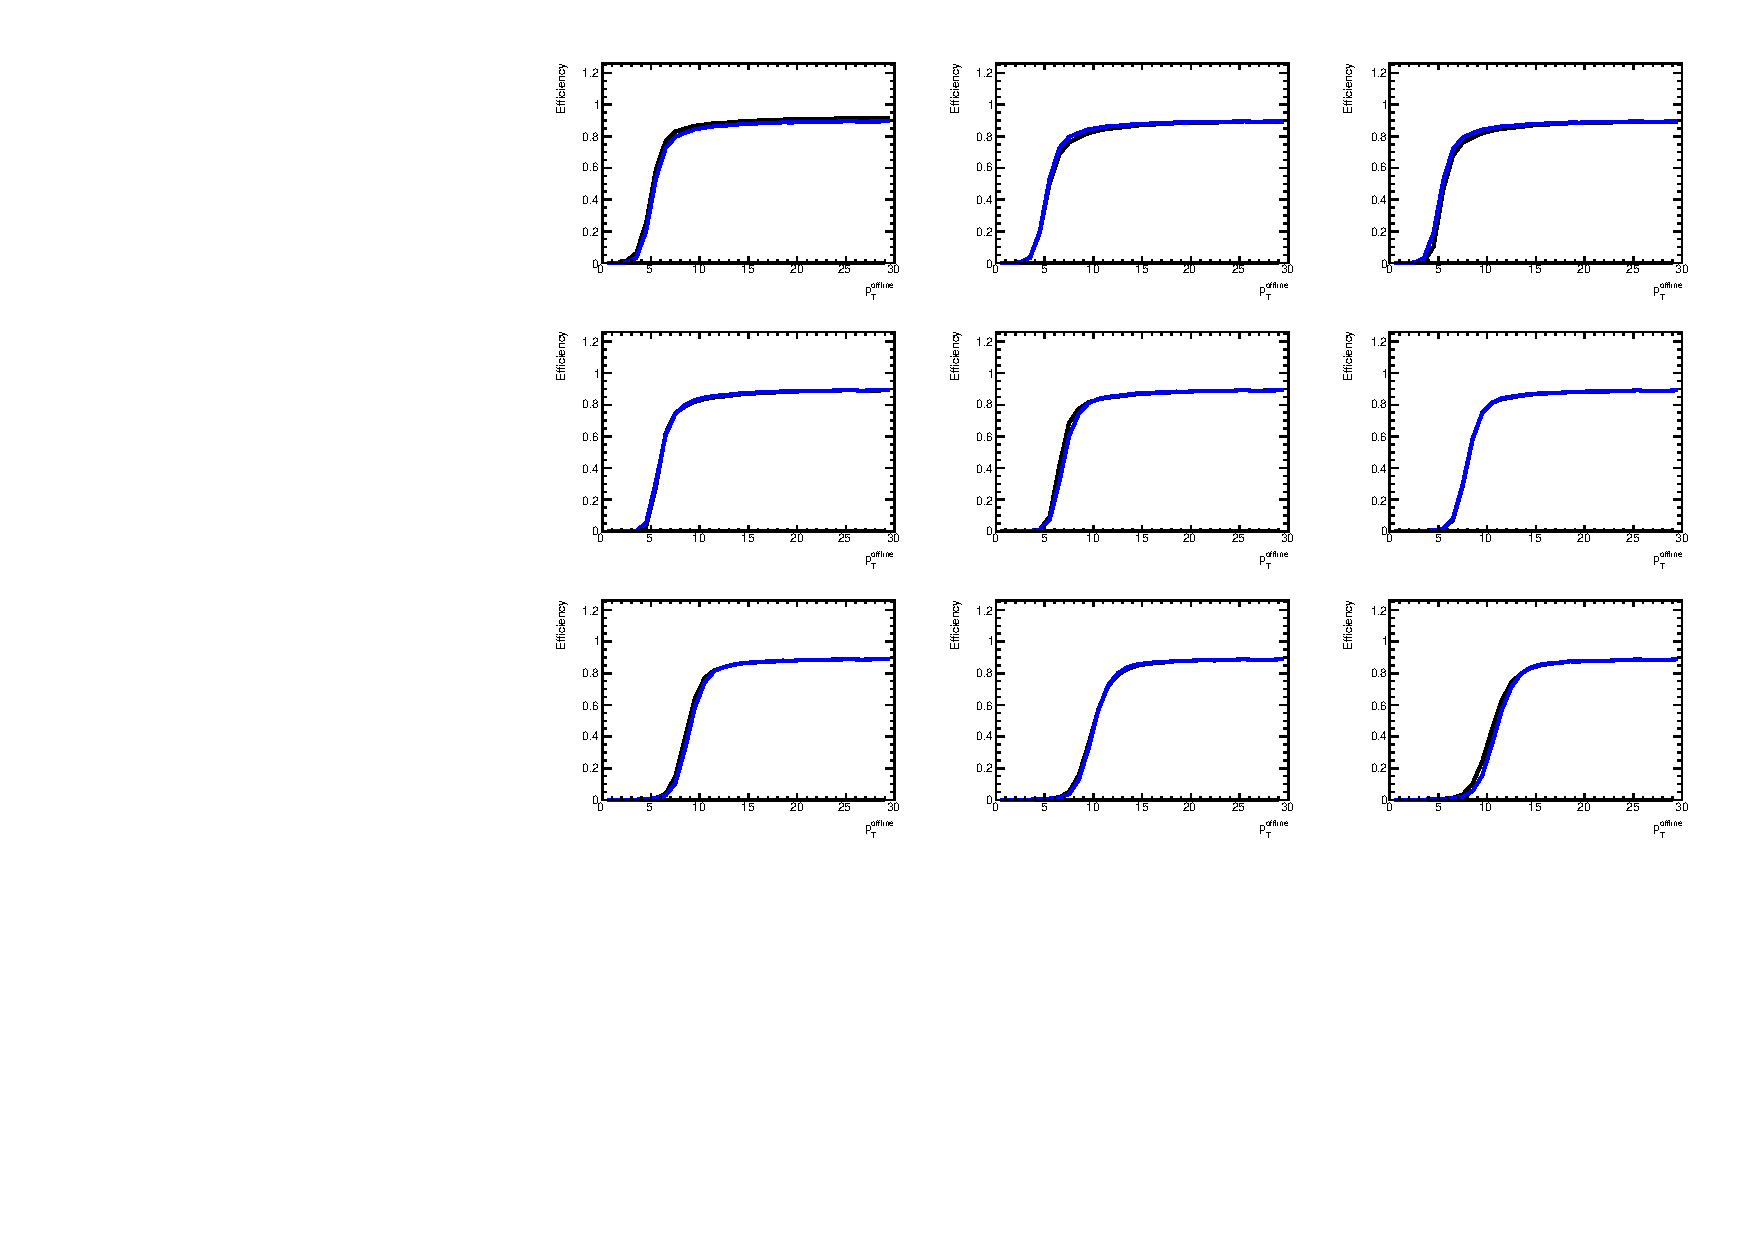
\includegraphics[clip, width=10cm]{fig/5/v05v07_1_9.pdf}
%  \caption{$p_{\rm{T}}$閾値3~GeV$\sim$9~GeVにおける$\mathrm{CW_{Simu}}$と$\mathrm{CW_{2022}}$のTurn-on curveの比較。評価にはシングルミューオンのシミュレーションデータを使用した。}
%  \label{fig:v05v07_1_9_Simu}
%\end{figure}

%\begin{figure}[htb]
%  \centering
%  %\rule{8cm}{6cm}
%  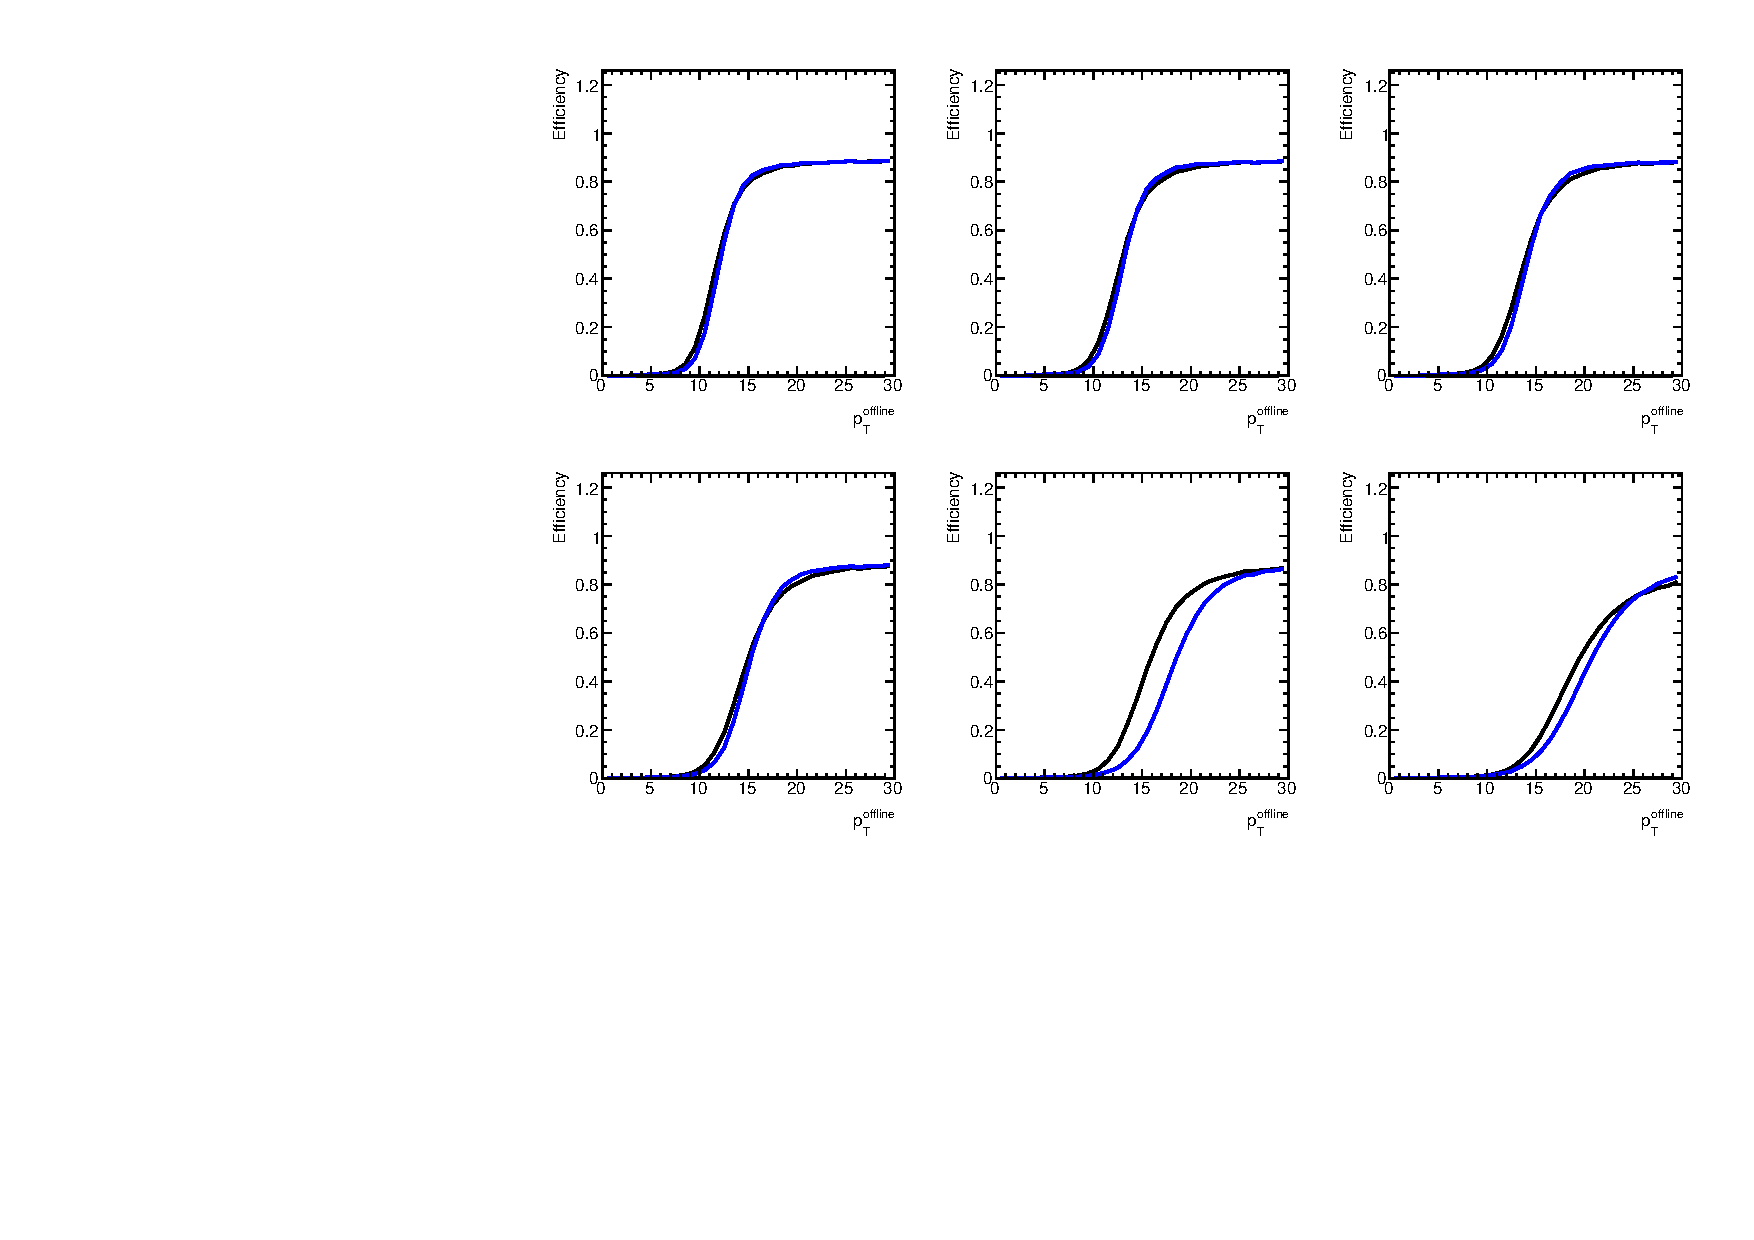
\includegraphics[clip, width=10cm]{fig/5/v05v07_10_15.pdf}
%  \caption{$p_{\rm{T}}$閾値10~GeV$\sim$20~GeVにおける$\mathrm{CW_{Simu}}$と$\mathrm{CW_{2022}}$のTurn-on curveの比較。評価にはシングルミューオンのシミュレーションデータを使用した。}
%  \label{fig:v05v07_12_20_Simu}
%\end{figure}

\begin{figure}[p]
  \centering
  %\rule{8cm}{6cm}
  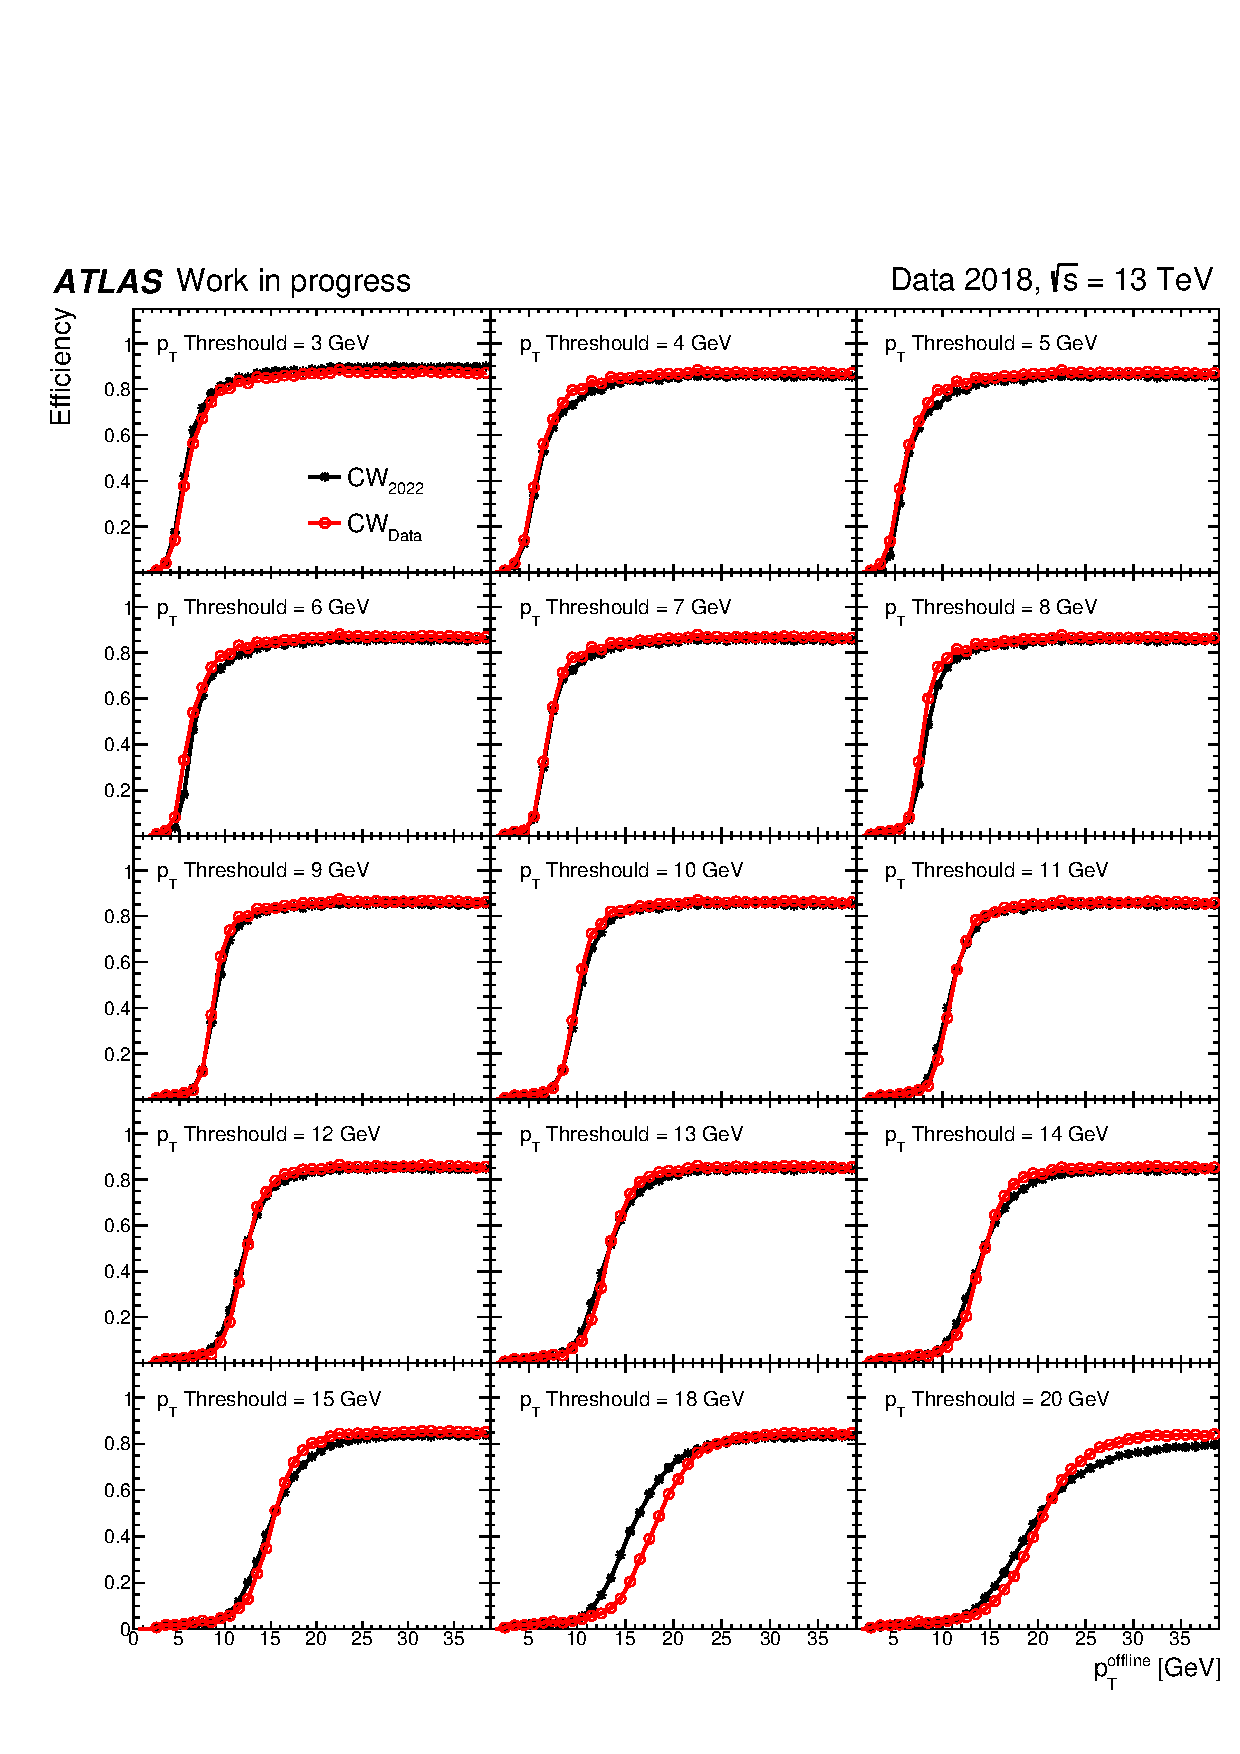
\includegraphics[clip, width=14cm]{fig/5/c1.pdf}
  \caption{$p_{\rm{T}}$閾値3~GeV$\sim$20~GeVにおける$\mathrm{CW_{Data}}$と$\mathrm{CW_{2022}}$のTurn-on curveの比較。評価には2018年Run-2のデータを使用した。}
  \label{fig:v05v06_1_9_Data}
\end{figure}

%\begin{figure}[htb]
%  \centering
%  %\rule{8cm}{6cm}
%  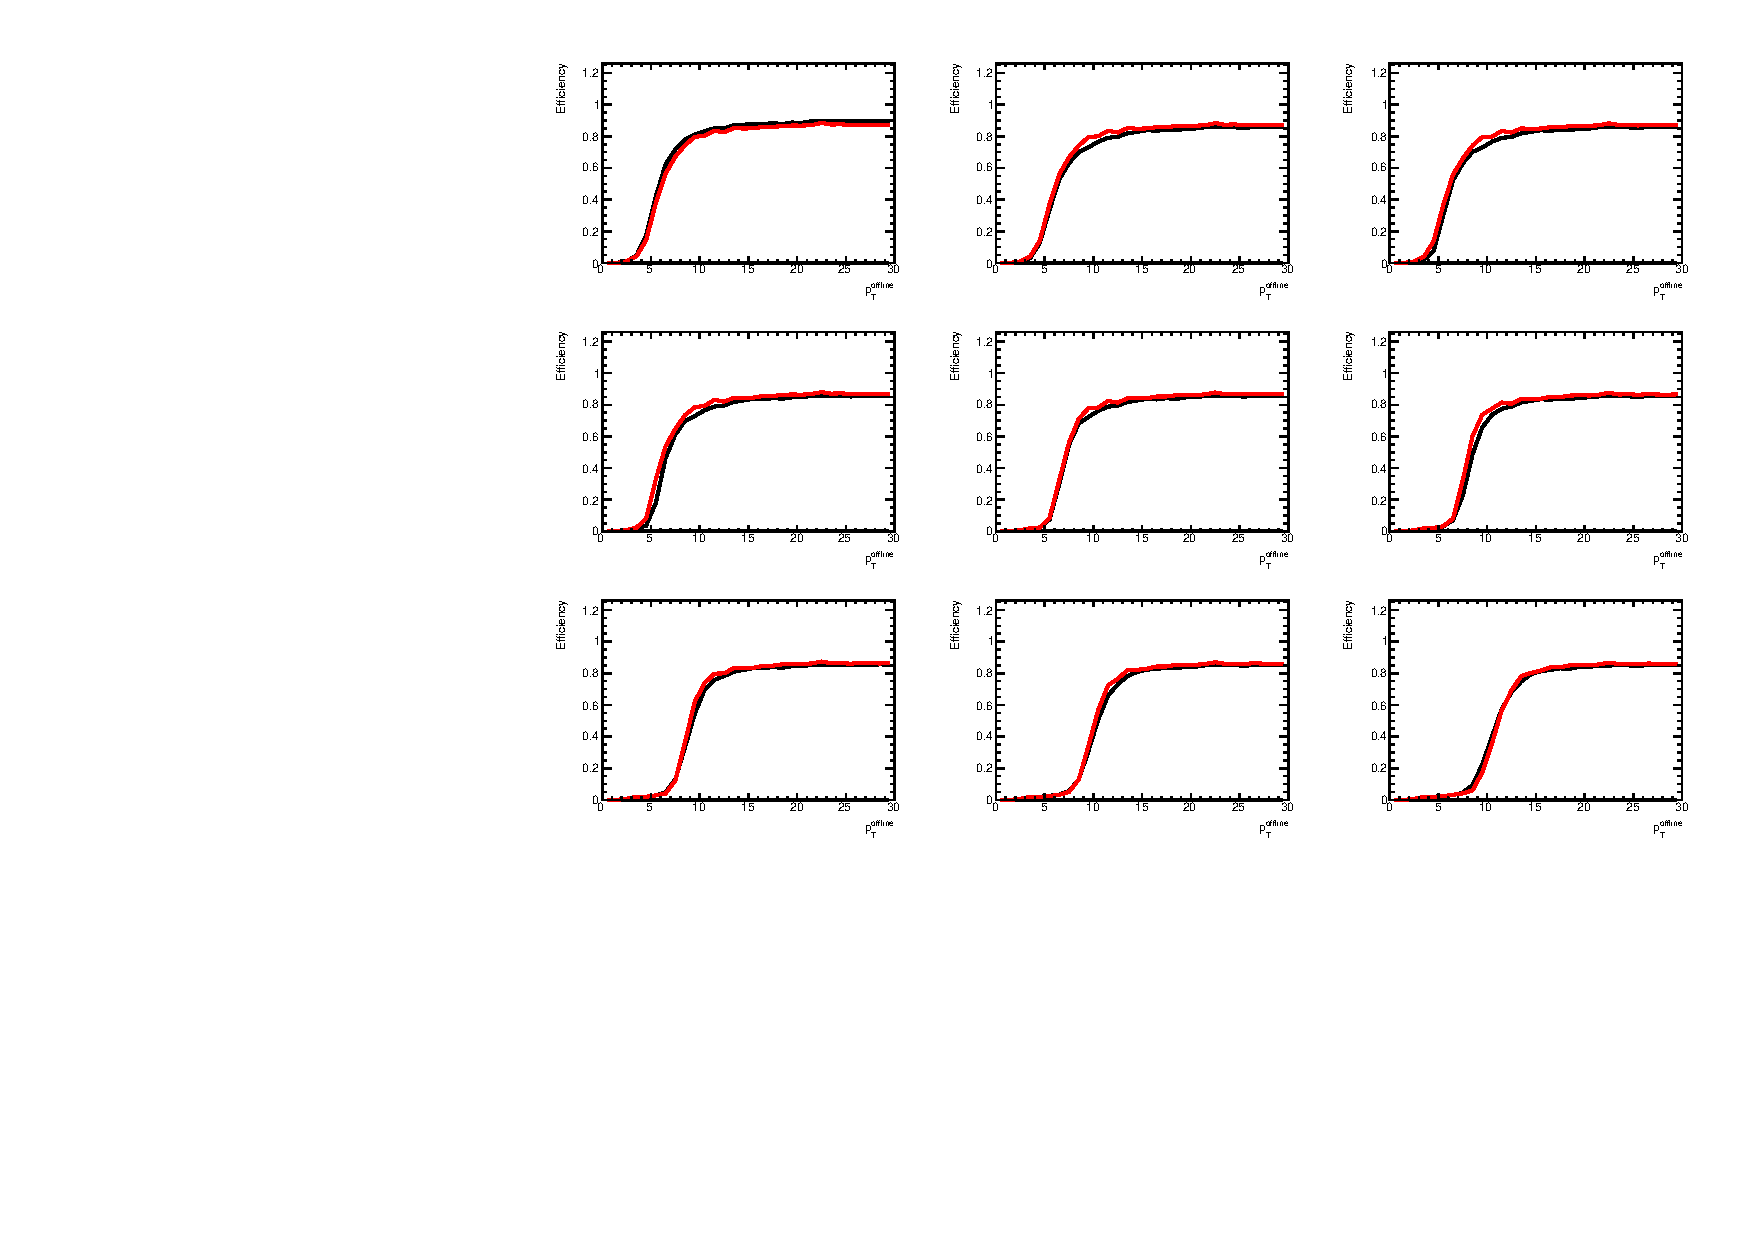
\includegraphics[clip, width=10cm]{fig/5/v05v06_1_9.pdf}
%  \caption{$p_{\rm{T}}$閾値3~GeV$\sim$ 9~GeVにおける$\mathrm{CW_{Data}}$と$\mathrm{CW_{2022}}$のTurn-on curveの比較。評価には2018年Run-3のデータを使用した。}
%  \label{fig:v05v06_1_9_Data}
%\end{figure}

%\begin{figure}[htb]
%  \centering
  %\rule{8cm}{6cm}
%  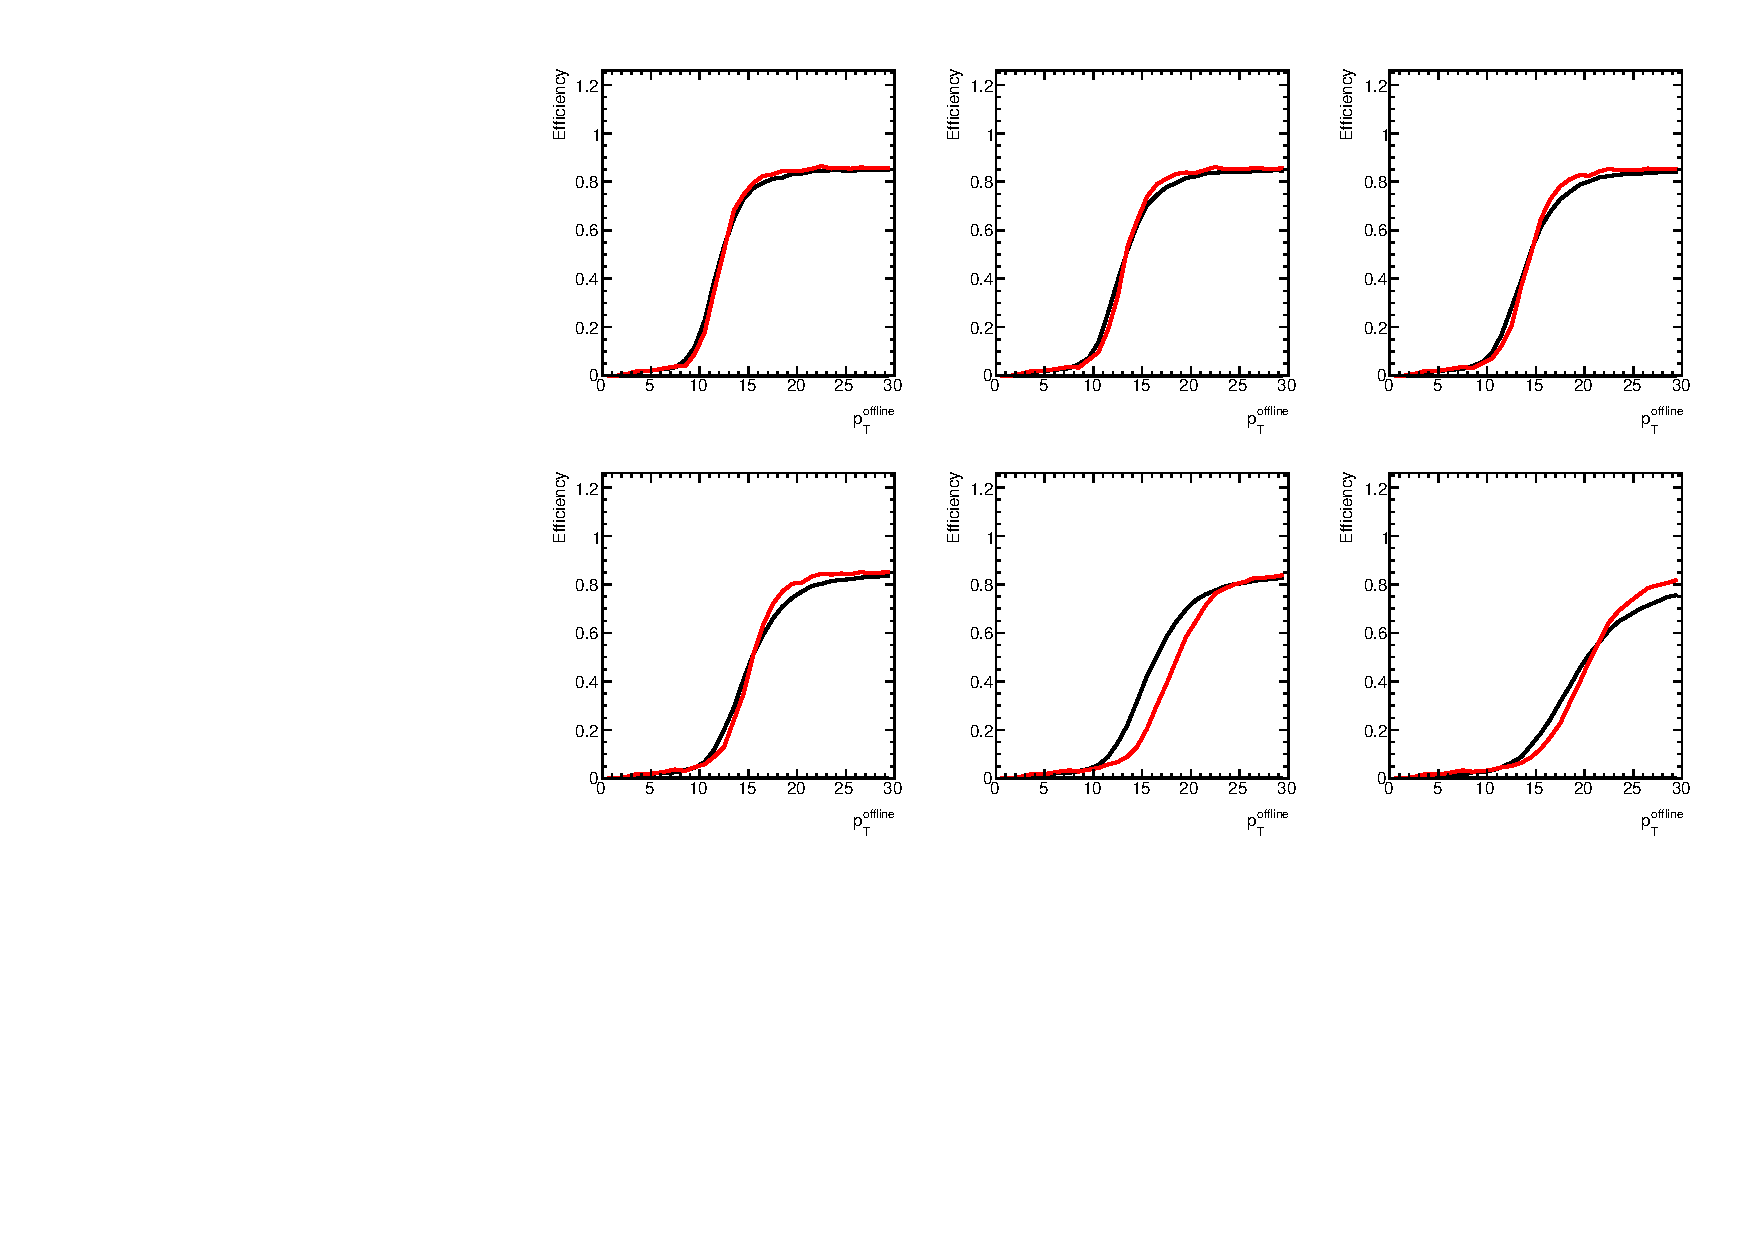
\includegraphics[clip, width=10cm]{fig/5/v05v06_10_15.pdf}
%  \caption{$p_{\rm{T}}$閾値10~GeV$\sim$ 20~GeVにおける$\mathrm{CW_{Data}}$と$\mathrm{CW_{2022}}$のTurn-on curveの比較。評価には2018年Run-3のデータを使用した。}
%  \label{fig:v05v06_10_15_Data}
%\end{figure}

さらに、これらのTurn-on curveに式~\eqref{equ:fitting}によるフィッティングを行い、パラメータの比較を行う。
図~\ref{fig:Resolution_v07v05}に$\mathrm{CW_{Simu}}$と$\mathrm{CW_{2022}}$の各$p_{\rm{T}}$閾値のResolitionの比較、図~\ref{fig:Resolution_v06v05}に$\mathrm{CW_{Data}}$と$\mathrm{CW_{2022}}$の各$p_{\rm{T}}$閾値のResolitionの比較を示す。
また、図~\ref{fig:Plateau_v07v05}に$\mathrm{CW_{Simu}}$と$\mathrm{CW_{2022}}$の各$p_{\rm{T}}$閾値のPlateau Efficiencyの比較、図~\ref{fig:Plateau_v06v05}に$\mathrm{CW_{Data}}$と$\mathrm{CW_{2022}}$の各$p_{\rm{T}}$閾値のPlateau Efficiencyの比較を示す。

まず、シミュレーションデータをトレーニングに用いて作成した$\mathrm{CW_{Simu}}$と2018年Run-3で使用された$\mathrm{CW_{2022}}$を比較すると、Resolition及びPlateau Efficiencyがほとんど一致していることがわかる。
このことから、本研究の手法は従来の手法と同様の性能を維持できるCWの作成が可能であることが確認できた。
次に、実際のデータをトレーニングにに使用した$\mathrm{CW_{Data}}$と2018年Run-3で使用された$\mathrm{CW_{2022}}$を比較すると、$p_{\rm{T}}$閾値が14~GeVのトリガーではResolitionが。q改善され、Plateau Efficiencyが約2$\%$向上したことが見て取れる。これは、実際のデータをトレーニングに用いたことで、検出器アライメントの最適化が行われたことを表している。

\begin{figure}
    %\centering
    \begin{tabular}{cc}
    \centering
    \begin{minipage}[b]{0.45\hsize}%
        \centering
        \hspace*{-1.5cm}
        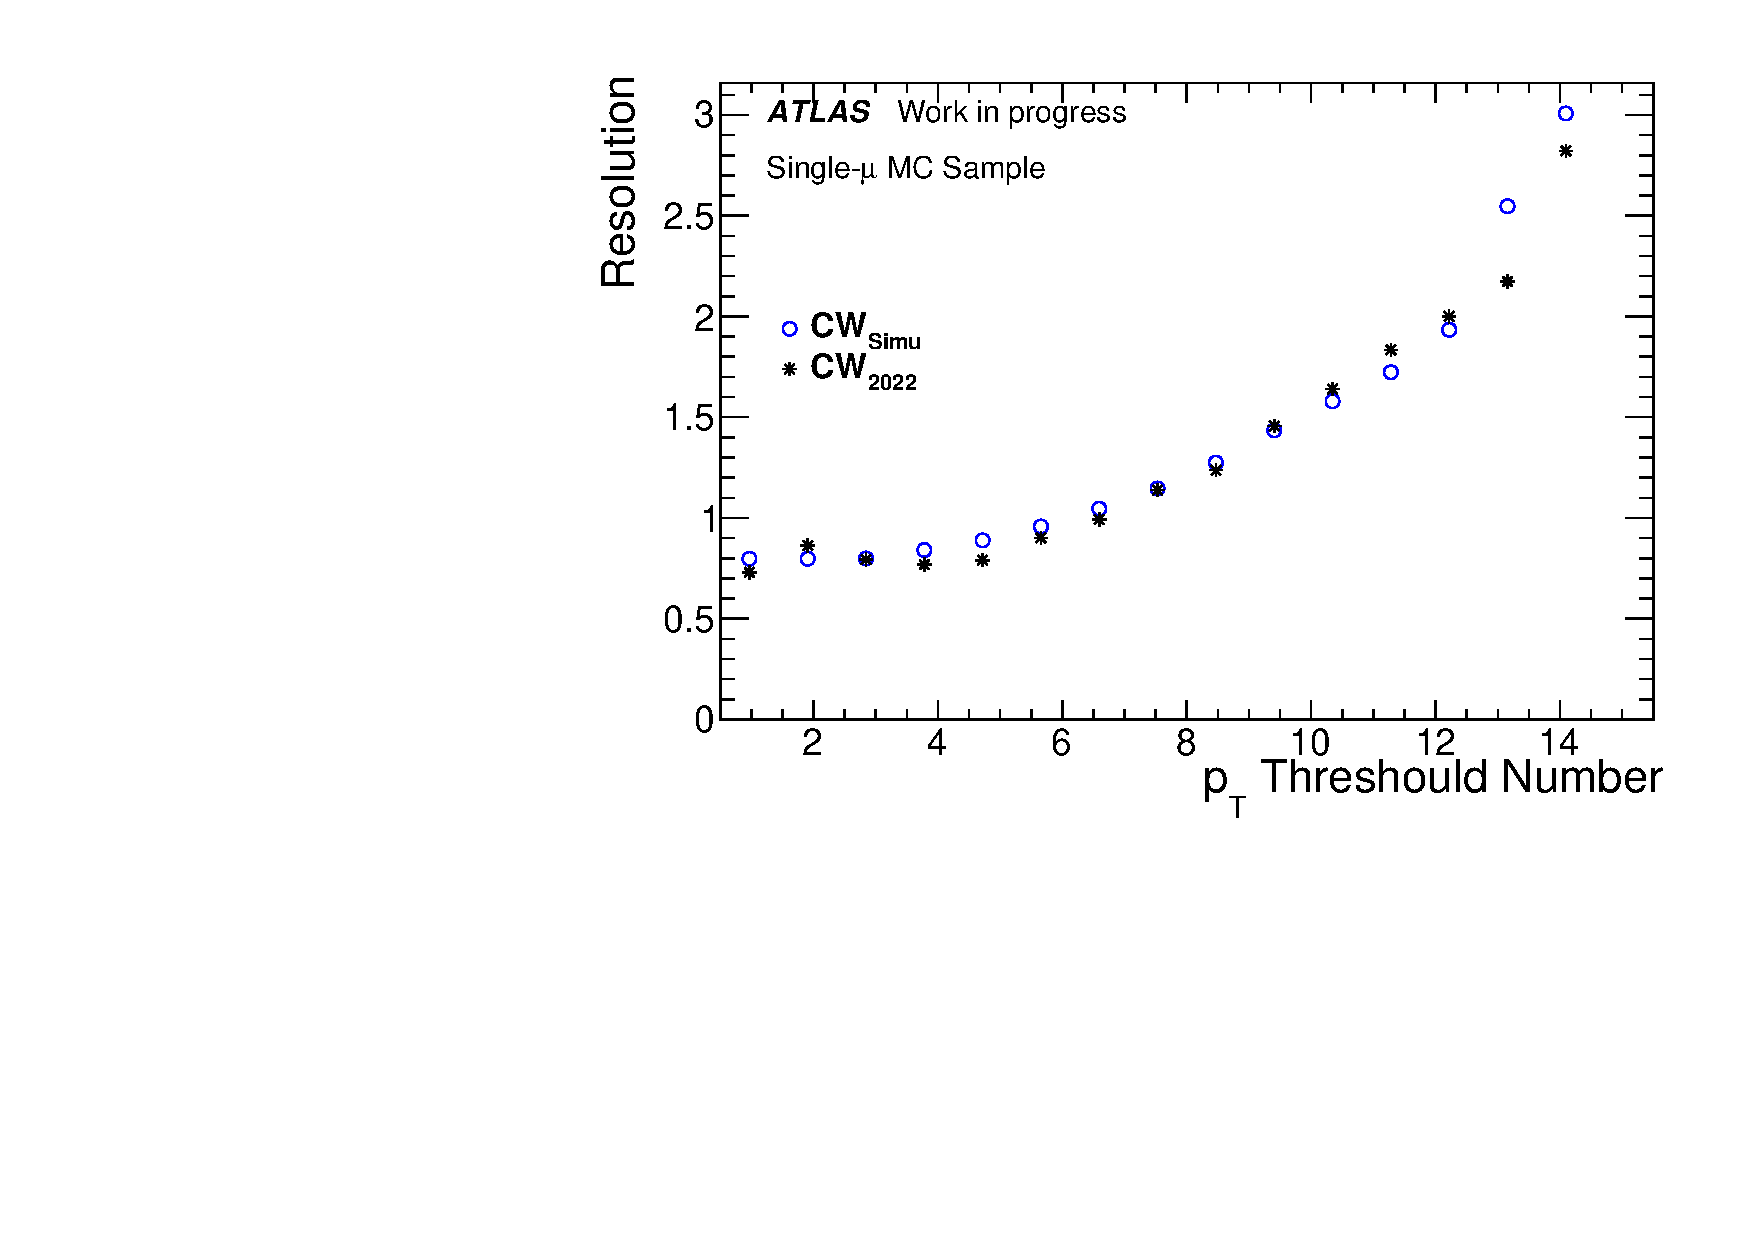
\includegraphics[clip, width=8cm]{fig/5/v05vsv07_Resolution_re.pdf}
        %\vspace{5pt}
        \subcaption{$\mathrm{CW_{Simu}}$と$\mathrm{CW_{2022}}$の比較。}
        \label{fig:Resolution_v07v05}
    \end{minipage}%
    %\hfill
    \begin{minipage}[b]{0.7\hsize}%
        \centering
        \hspace*{-0.75cm}
        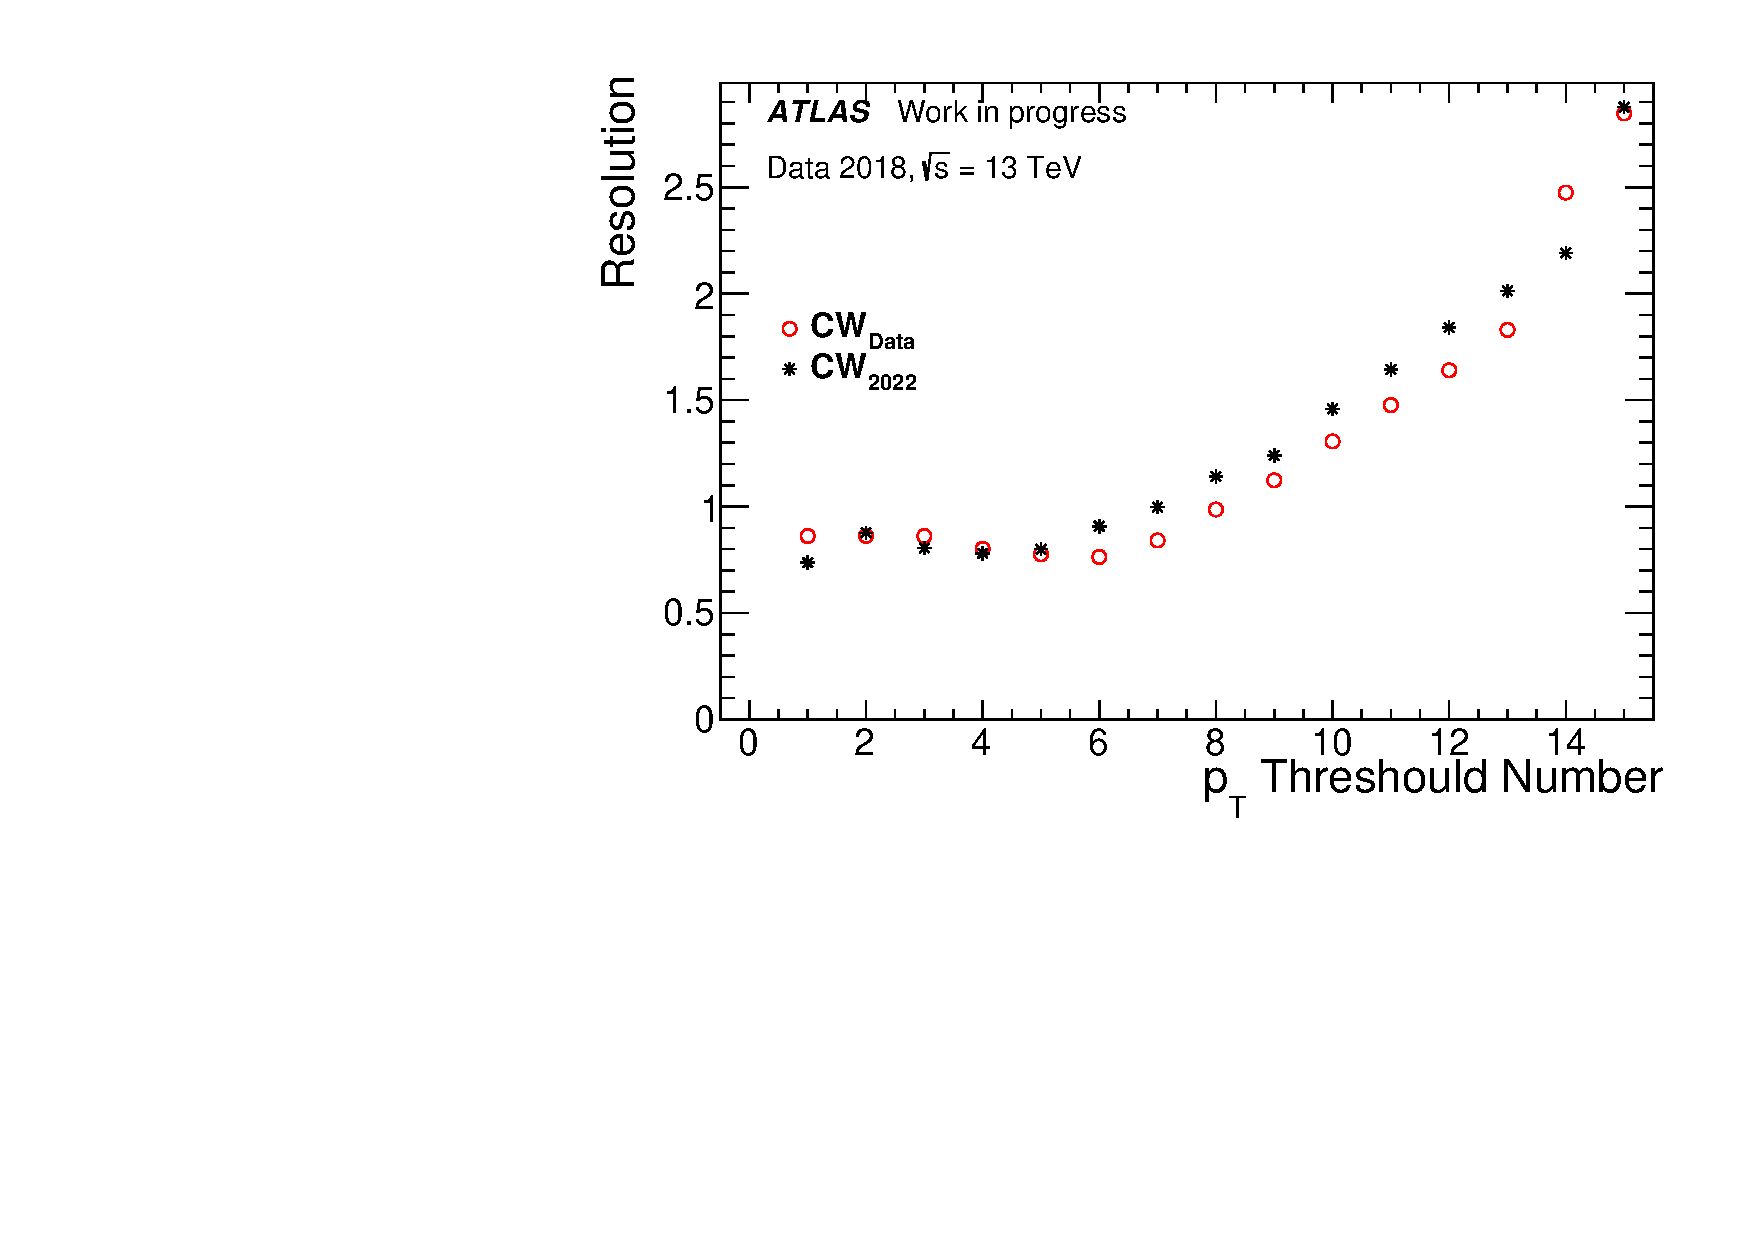
\includegraphics[clip, width=8cm]{fig/5/v05vsv06_Resolution_re.pdf}
        %\vspace{5pt}
        \subcaption{$\mathrm{CW_{Data}}$と$\mathrm{CW_{2022}}$の比較。}
        \label{fig:Resolution_v06v05}
    \end{minipage}%
    \end{tabular}
    \caption{各$p_{\rm{T}}$閾値におけるResolutionの比較。}
    \label{fig:Resolution_v07v06v05}
\end{figure}

\begin{figure}
    %\centering
    \begin{tabular}{cc}
    \centering
    \begin{minipage}[b]{0.45\hsize}%
        \centering
        \hspace*{-1.5cm}
        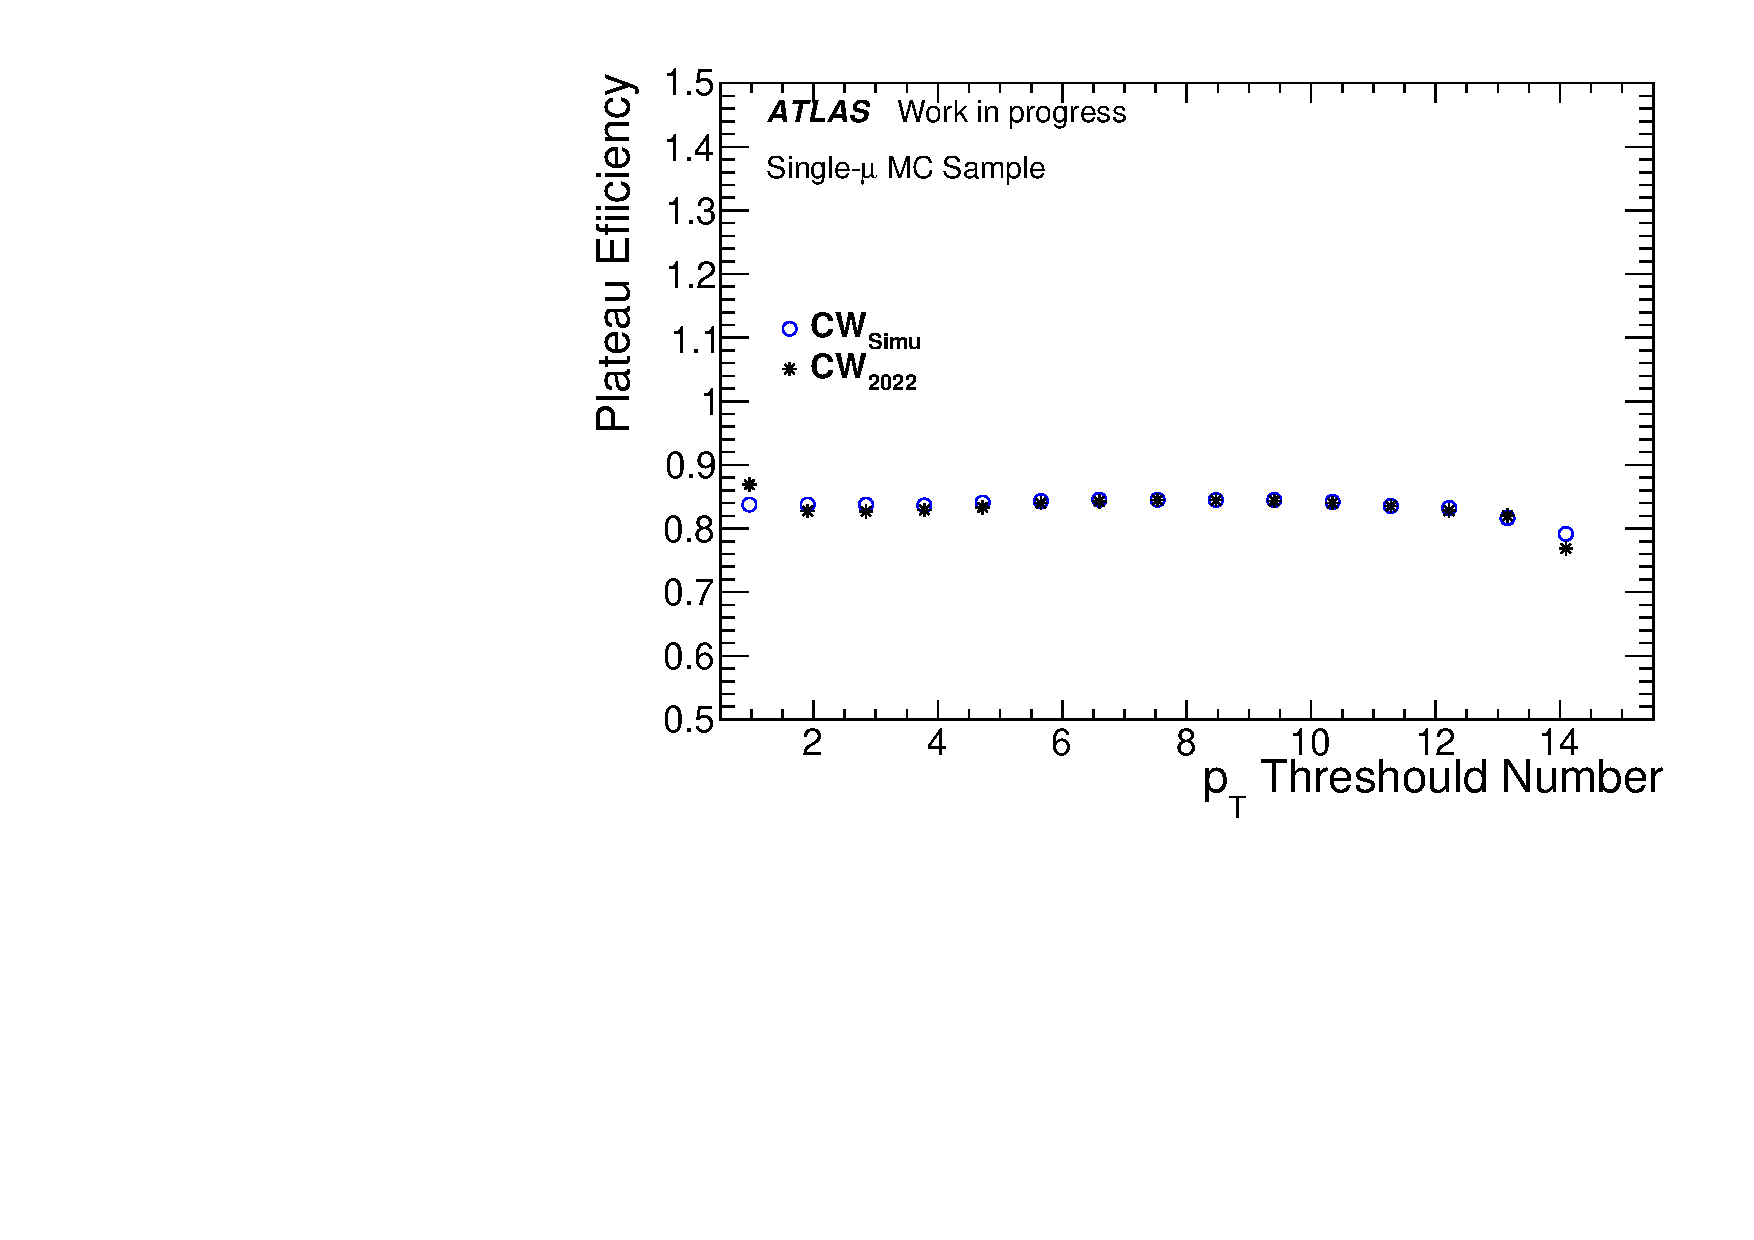
\includegraphics[clip, width=8cm]{fig/5/v05vsv07_Plateau_re.pdf}
        %\vspace{5pt}
        \subcaption{$\mathrm{CW_{Simu}}$と$\mathrm{CW_{2022}}$の比較}
        \label{fig:Plateau_v07v05}
    \end{minipage}%
    %\hfill
    \begin{minipage}[b]{0.7\hsize}%
        \centering
        \hspace*{-0.75cm}
        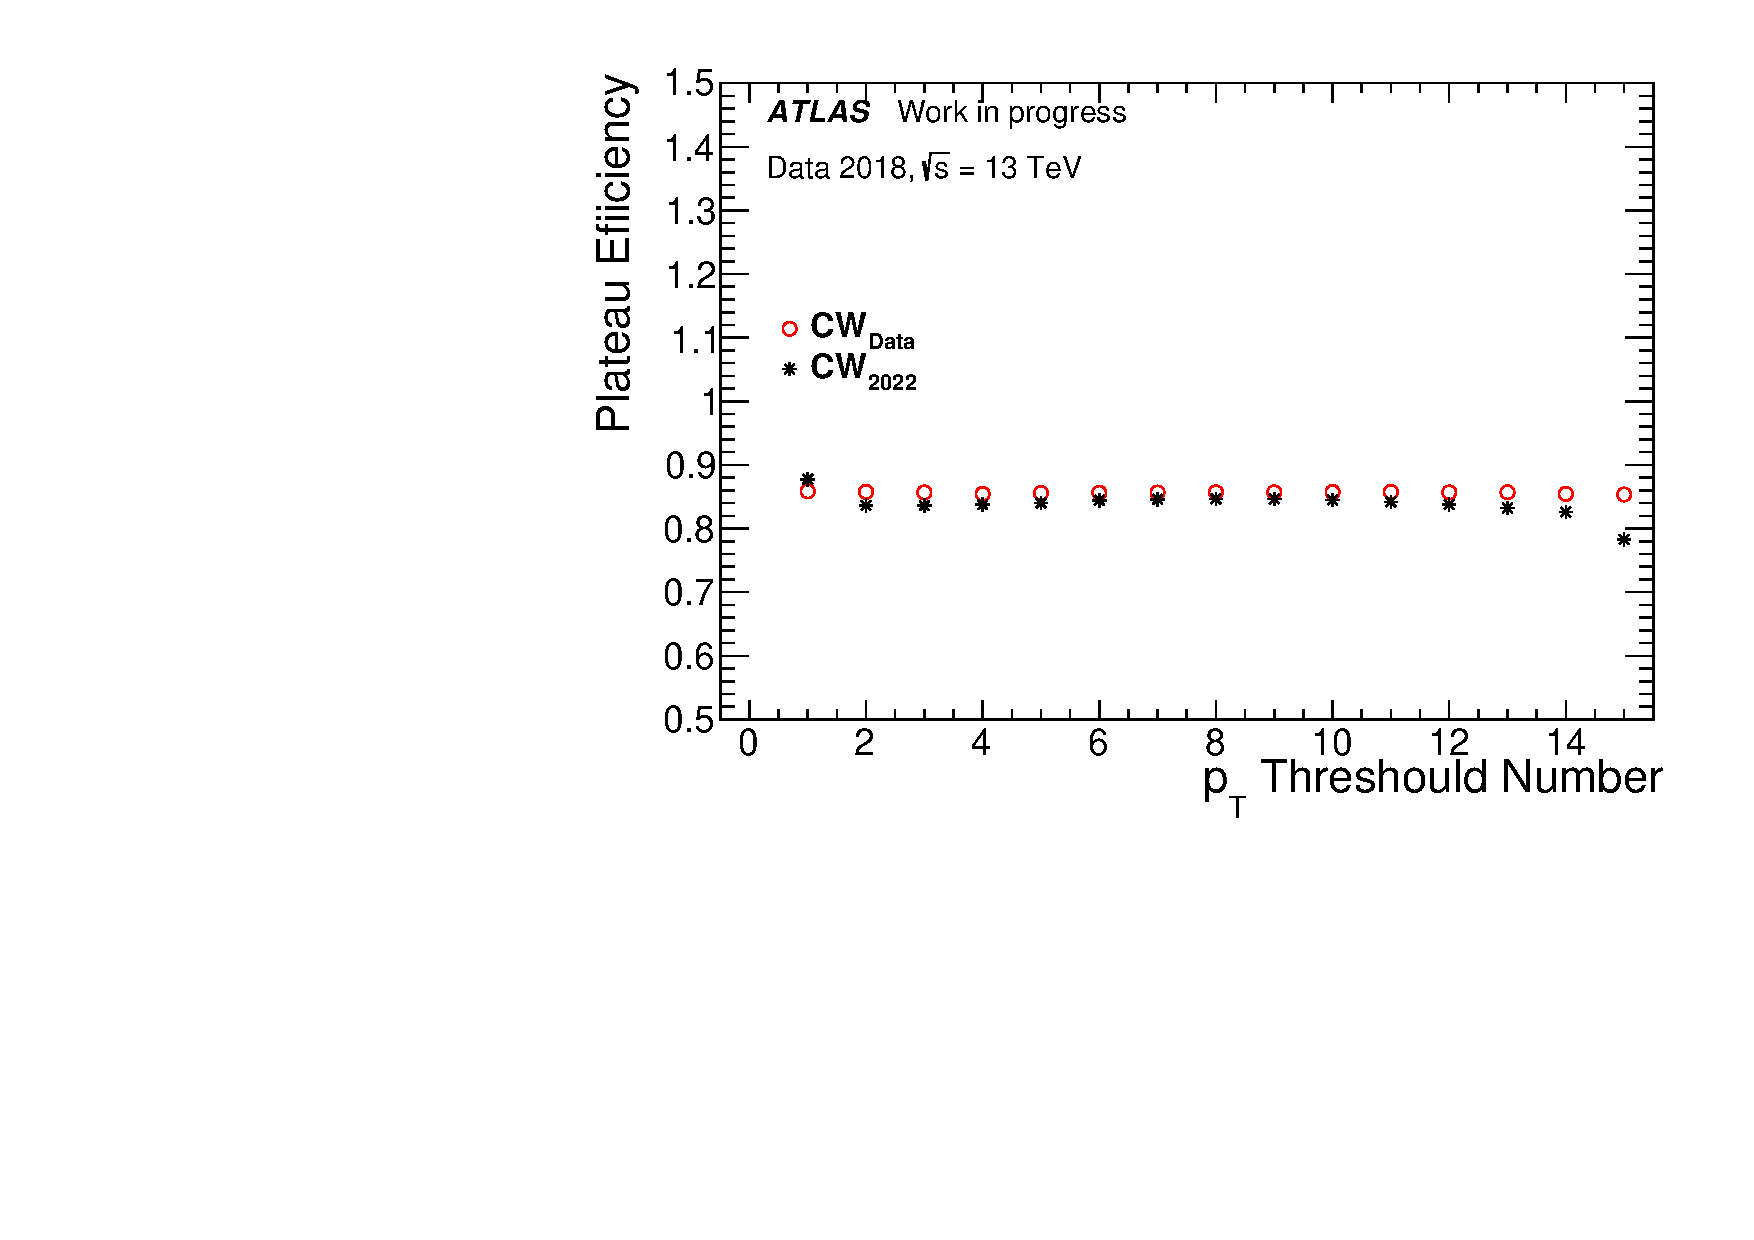
\includegraphics[clip, width=8cm]{fig/5/v05vsv06_Plateau_re.pdf}
        %\vspace{5pt}
        \subcaption{$\mathrm{CW_{Data}}$と$\mathrm{CW_{2022}}$の比較}
        \label{fig:Plateau_v06v05}
    \end{minipage}%
    \end{tabular}
    \caption{各$p_{\rm{T}}$閾値におけるPlateau Efficiencyの比較。}
    \label{fig:Resolution_v07v06v05}
\end{figure}

\subsubsection{$p_{\rm{T}}^{\rm{offline}}$分解能の評価}\label{分解能の評価}
$p_{\rm{T}}$分解能を式~\eqref{equ:residual}で計算する$p_{\rm{T}}$ residualを用いて評価する。
\begin{equation}
    p_{\rm{T}} residual = \frac{p_{\rm{T}}^{\rm{L1}}-p_{\rm{T}}^{offline}}{p_{\rm{T}}^{offline}}
    \label{equ:residual}
\end{equation}
ここで、$p_{\rm{T}}^{L1}$はL1MuonでCWを用いて判定される$p_{\rm{T}}$閾値、$p_{\rm{T}}^{\rm{offline}}$はオフライン再構成されたミューオンで$p_{\rm{T}}$ある。
そのため、$p_{\rm{T}}^{\rm{offline}}$に対して正しく$p_{\rm{T}}^{L1}$を判定できていれば0に近づき、0から離れるほど$p_{\rm{T}}^{L1}$が$p_{\rm{T}}^{\rm{offline}}$とずれていることになる。

この$p_{\rm{T}}$ residualを1~GeVごとの$p_{\rm{T}}^{\rm{offline}}$に対して計算し、細かい$p_{\rm{T}}$に対する分解能の評価を行う。
まず、本研究の手法で作成した$\mathrm{CW_{Simu}}$と2022年度Run-2で使用された$\mathrm{CW_{2022}}$の比較を行う。
図~\ref{residual_MC_3_18}に1~GeVごとの$p_{\rm{T}}^{\rm{offline}}$に対する$p_{\rm{T}}$ residual分布を示す。
\begin{figure}[htbp]
  \centering
  %\rule{8cm}{6cm}
  \hspace*{-1cm}
  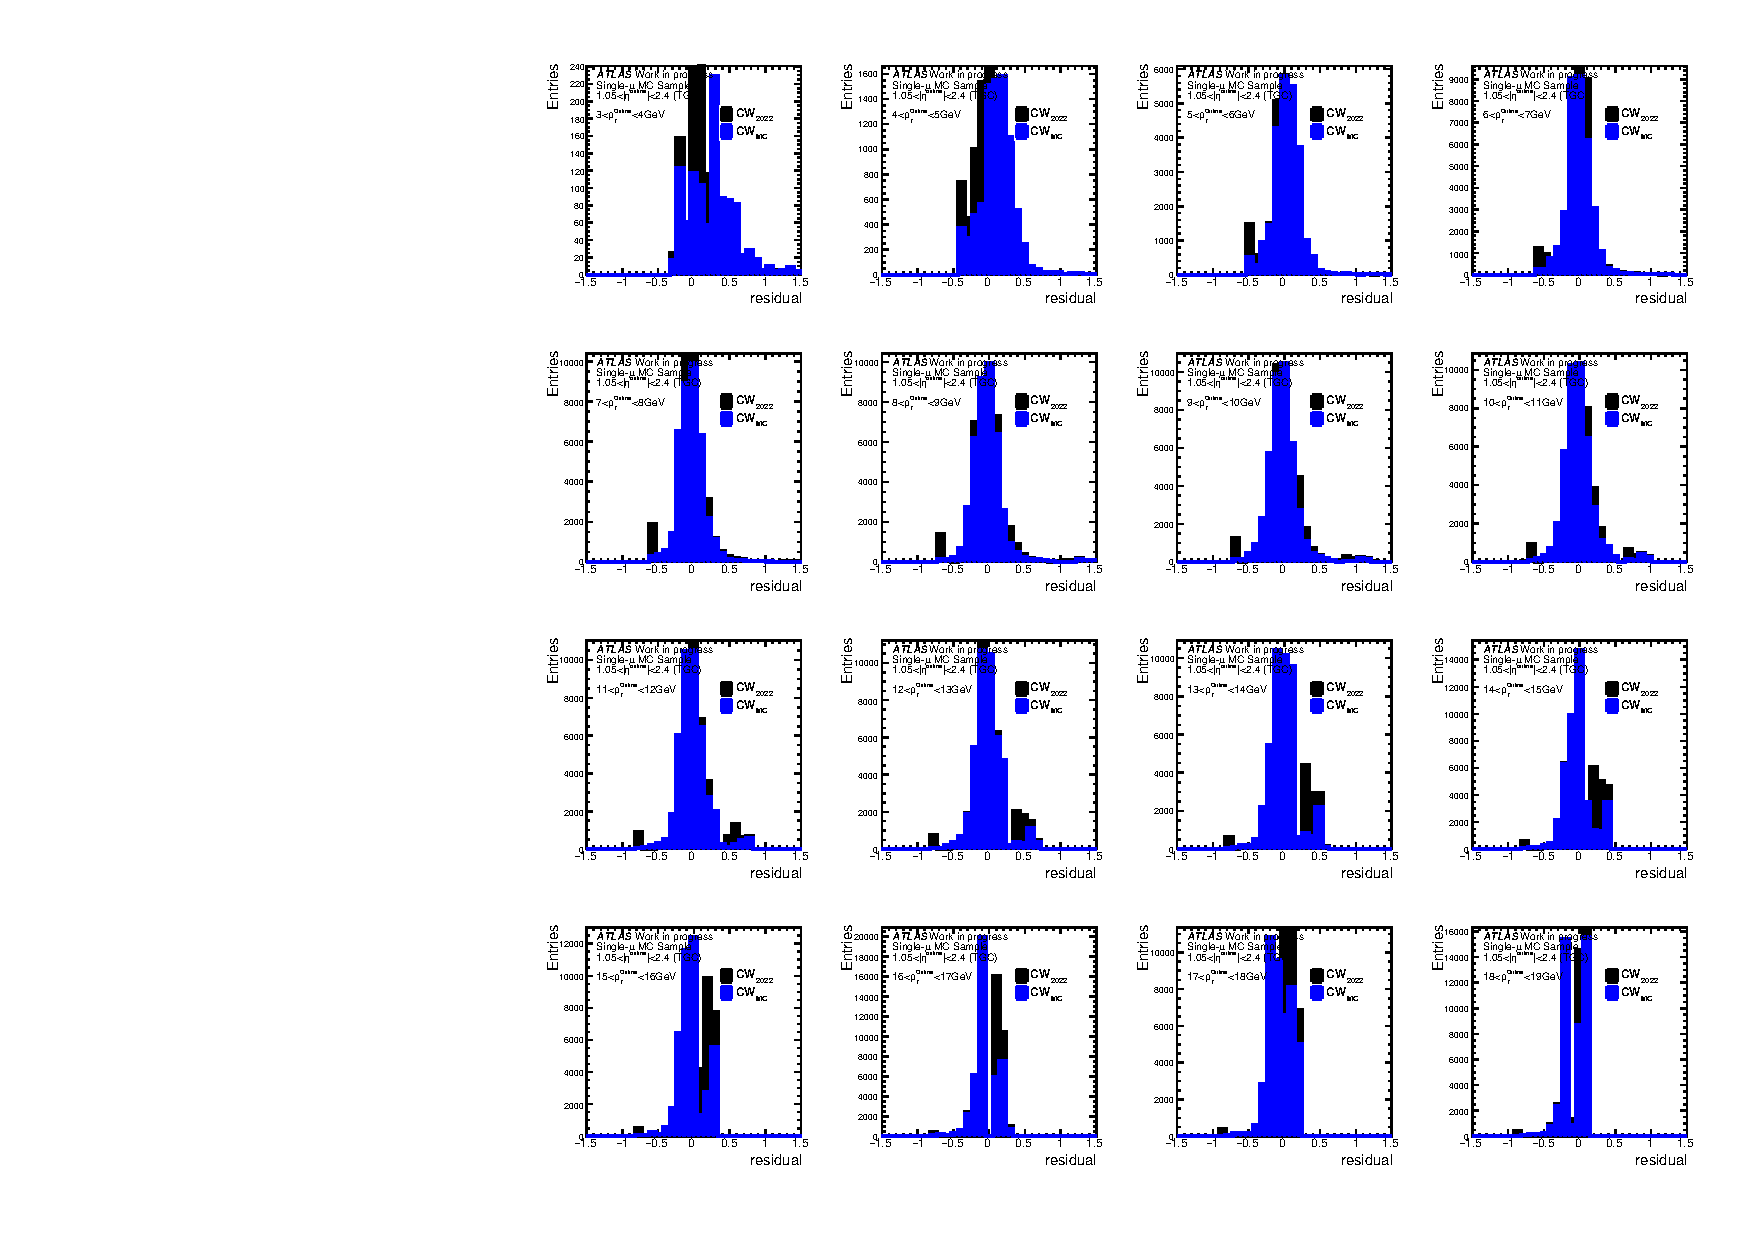
\includegraphics[clip, width=16cm]{fig/5/residual_MC_3_18.pdf}
  \caption{TGCにおける1GeV刻みのpT residual分布(3$\sim$18~GeV)。青が本研究の手法で作成した$\mathrm{CW_{Simu}}$を用いた結果、黒が2022年度Run-2で使用された$\mathrm{CW_{2022}}$を用いた結果である。}
  \label{residual_MC_3_18}
\end{figure}
%\begin{figure}[htb]
%  \centering
%  %\rule{8cm}{6cm}
%  \hspace*{-1cm}
%  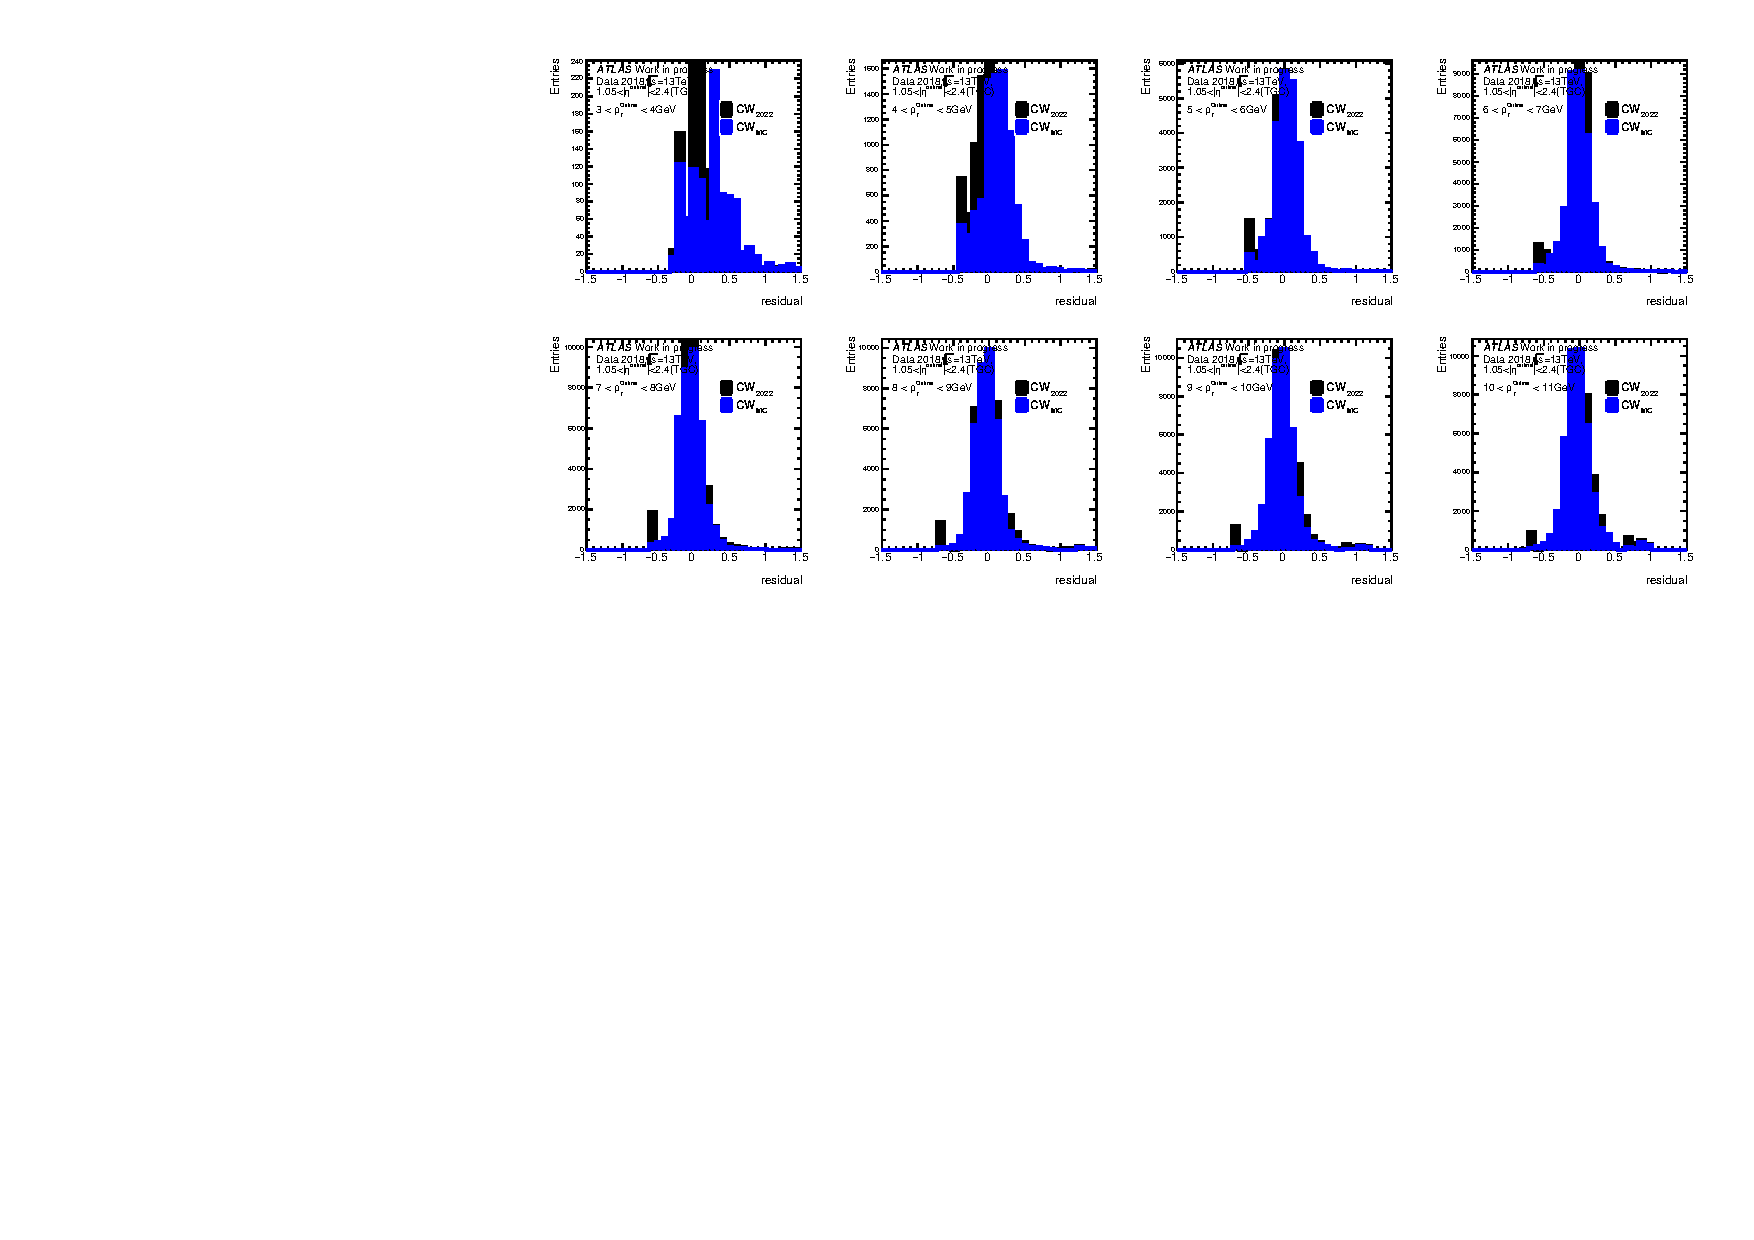
\includegraphics[clip, width=16cm]{fig/5/residual_MC_3_10.pdf}
%  \caption{TGCにおける1GeV刻みのpT residual分布(3$\sim$10~GeV)。青が本研究の手法で作成した$\mathrm{CW_{Simu}}$を用いた結果、黒が2022年度Run-2で使用された$\mathrm{CW_{2022}}$を用いた結果である。}
%  \label{residual_MC_3_10}
%\end{figure}
%\begin{figure}[htb]
%  \centering
  %\rule{8cm}{6cm}
%  \hspace*{-1cm}
%  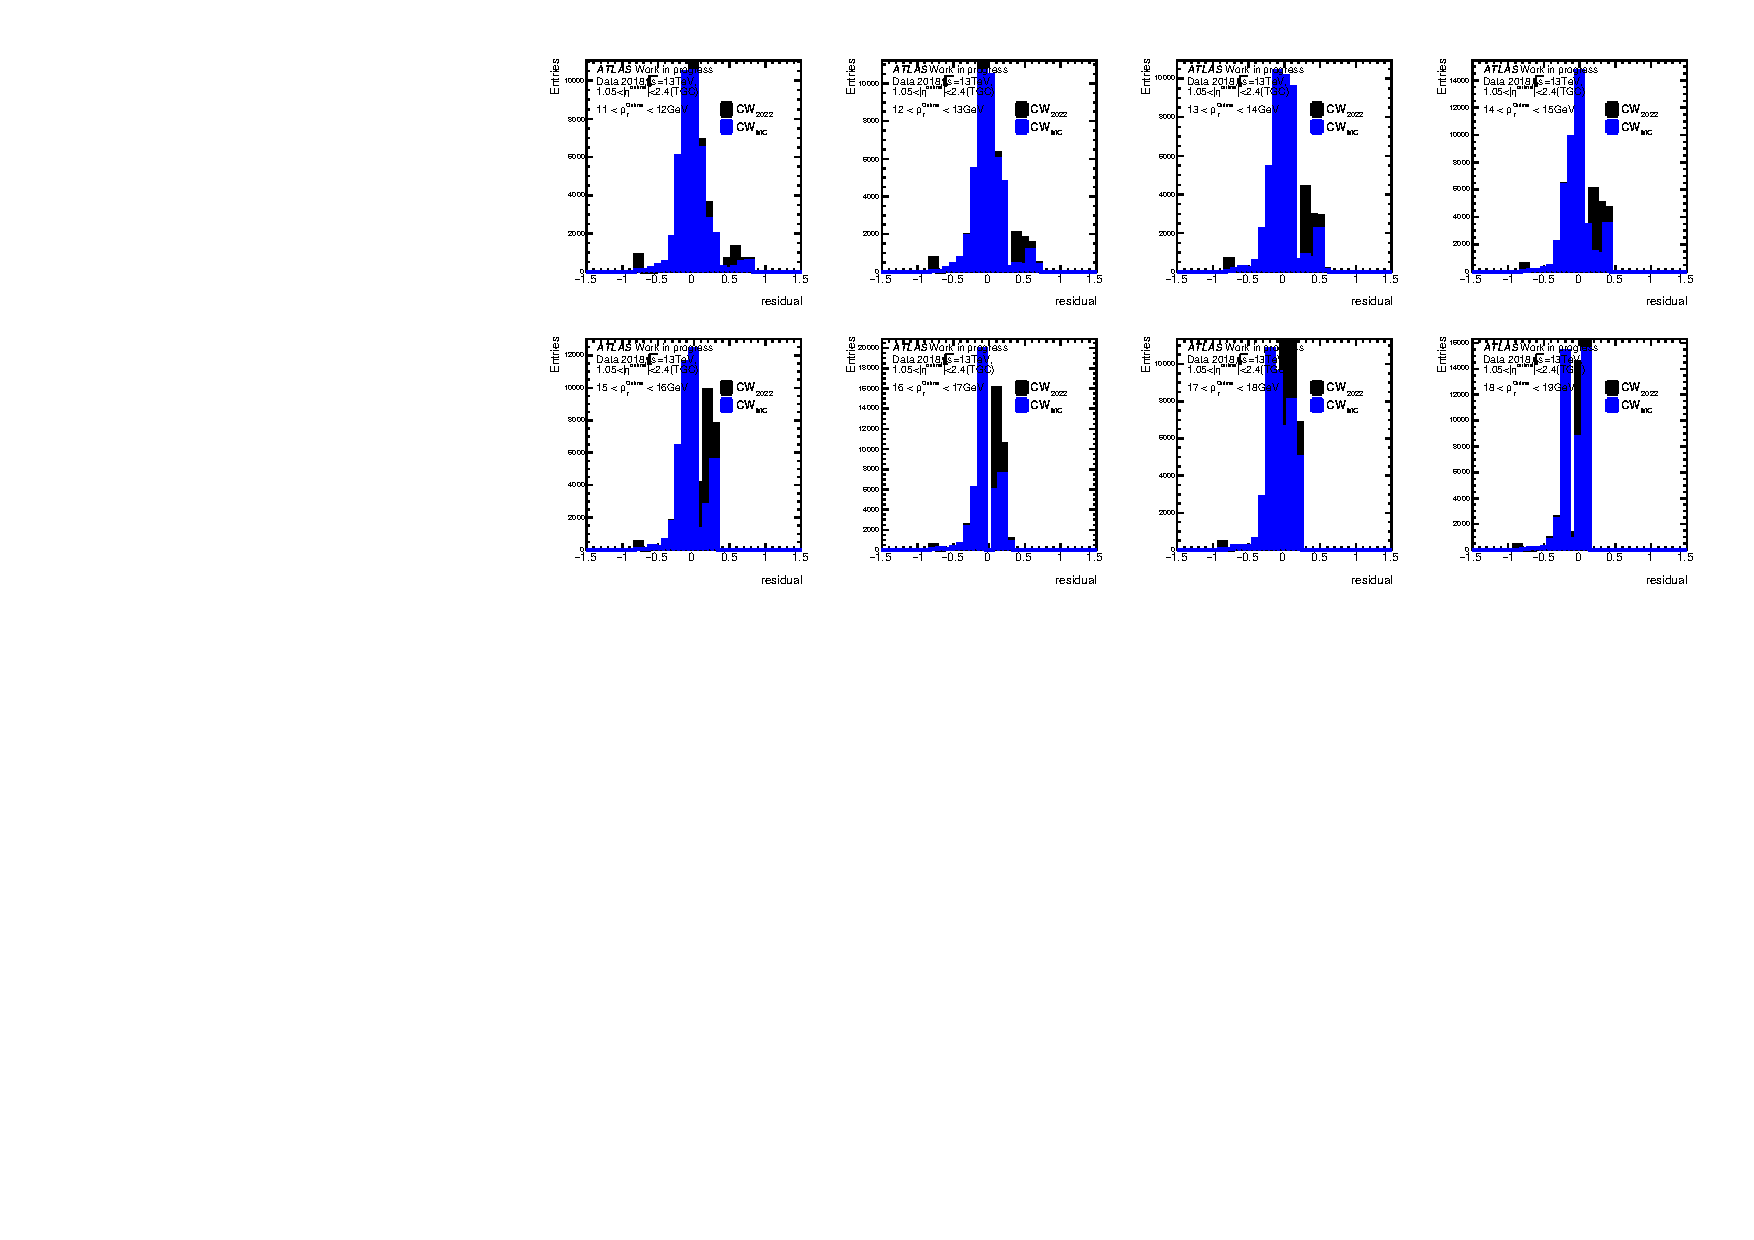
\includegraphics[clip, width=16cm]{fig/5/residual_MC_11_18.pdf}
%  \caption{TGCにおける1GeV刻みのpT residual分布(11$\sim$18~GeV)。青が本研究の手法で作成した$\mathrm{CW_{Simu}}$を用いた結果、黒が2022年度Run-3で使用された$\mathrm{CW_{2022}}$を用いた結果である。}
%  \label{residual_MC_11_18}
%\end{figure}
図~\ref{residual_MC}には1~GeV刻みの$p_{\rm{T}}$ residual分布のMean値と標準偏差を示した。
$\mathrm{CW_{2022}}$と比べ$\mathrm{CW_{Simu}}$は同程度のパフォーマンスが得られることが確認できる。
一方で低い$p_{\rm{T}}$に対する$p_{\rm{T}}^{\rm{offline}}$分解能は$\mathrm{CW_{2022}}$と比べて悪くなっている。これは、$p_{\rm{T}}$閾値の選択方法の影響が表れていると考えられる。
$\mathrm{CW_{2022}}$を作成した先行研究~\cite{article:shiomi-mron}では、この$p_{\rm{T}}^{\rm{offline}}$分解能が向上するような$p_{\rm{T}}$閾値の選択方法を確立し、15段階の$p_{\rm{T}}$閾値を選んでいた。そのため、本研究において$p_{\rm{T}}^{\rm{offline}}$分解能を評価した時、$\mathrm{CW_{2022}}$よりも悪化してしまったと考えられる。
本研究の手法は機械学習の出力からの$p_{\rm{T}}$閾値の選択方法を変えることで、$p_{\rm{T}}$閾値の15段階を柔軟に選択できる。そのため、図~\ref{fig:resi_std_Simu}に示すように$\mathrm{CW_{2022}}$と同程度以上の標準偏差を得られていることから、$\mathrm{CW_{2022}}$と同程度の以上の$p_{\rm{T}}^{\rm{offline}}$分解能を持つような$p_{\rm{T}}$閾値に対応できると見込まれる。

\begin{figure}
    %\centering
    \begin{tabular}{cc}
    \begin{minipage}[b]{0.45\hsize}
        %\centering
        \hspace*{-1cm}
        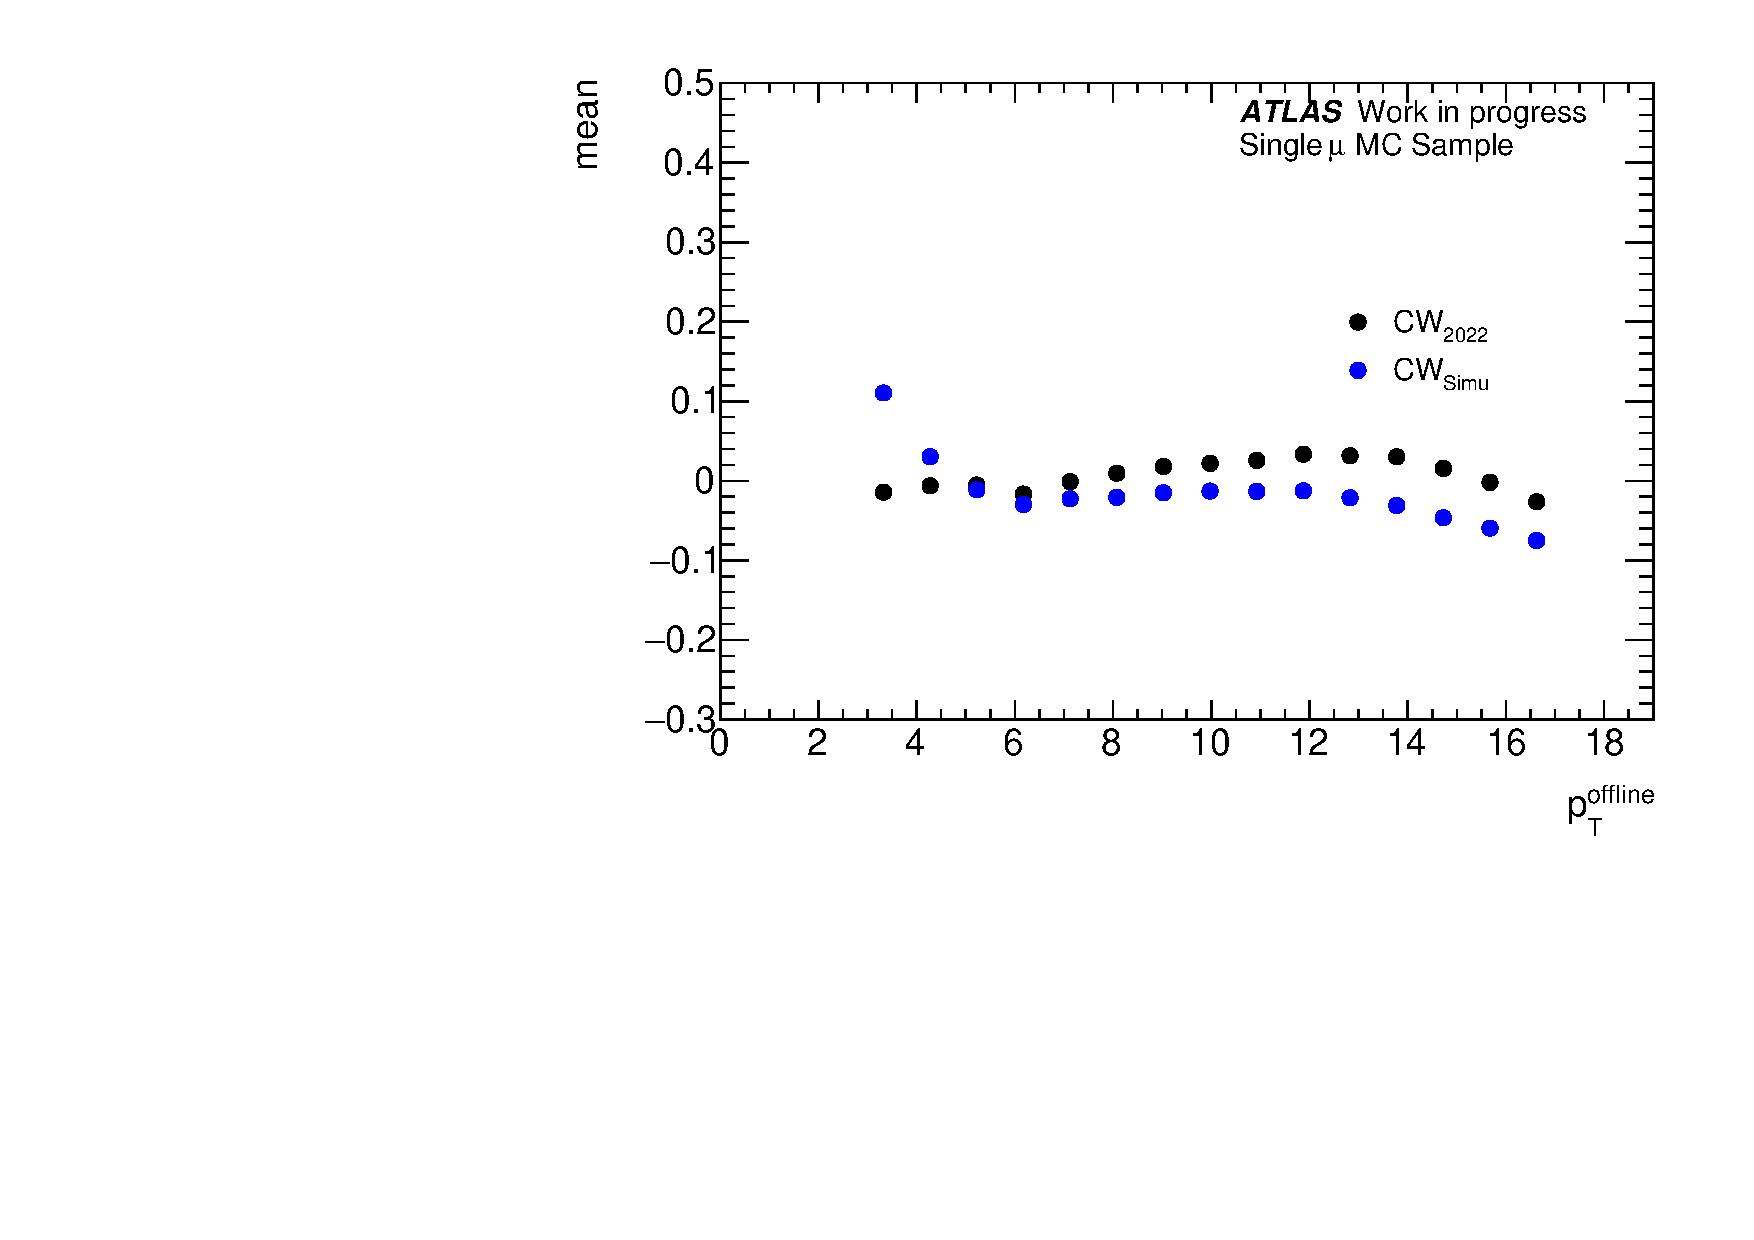
\includegraphics[clip, width=8cm]{fig/5/residual_mean_Simu.pdf}
        %\vspace{5pt}
        \subcaption{Mean値}
        \label{fig:resi_mean_Simu}
    \end{minipage}&
    %\hfill
    \begin{minipage}[b]{0.55\hsize}
        %\centering
        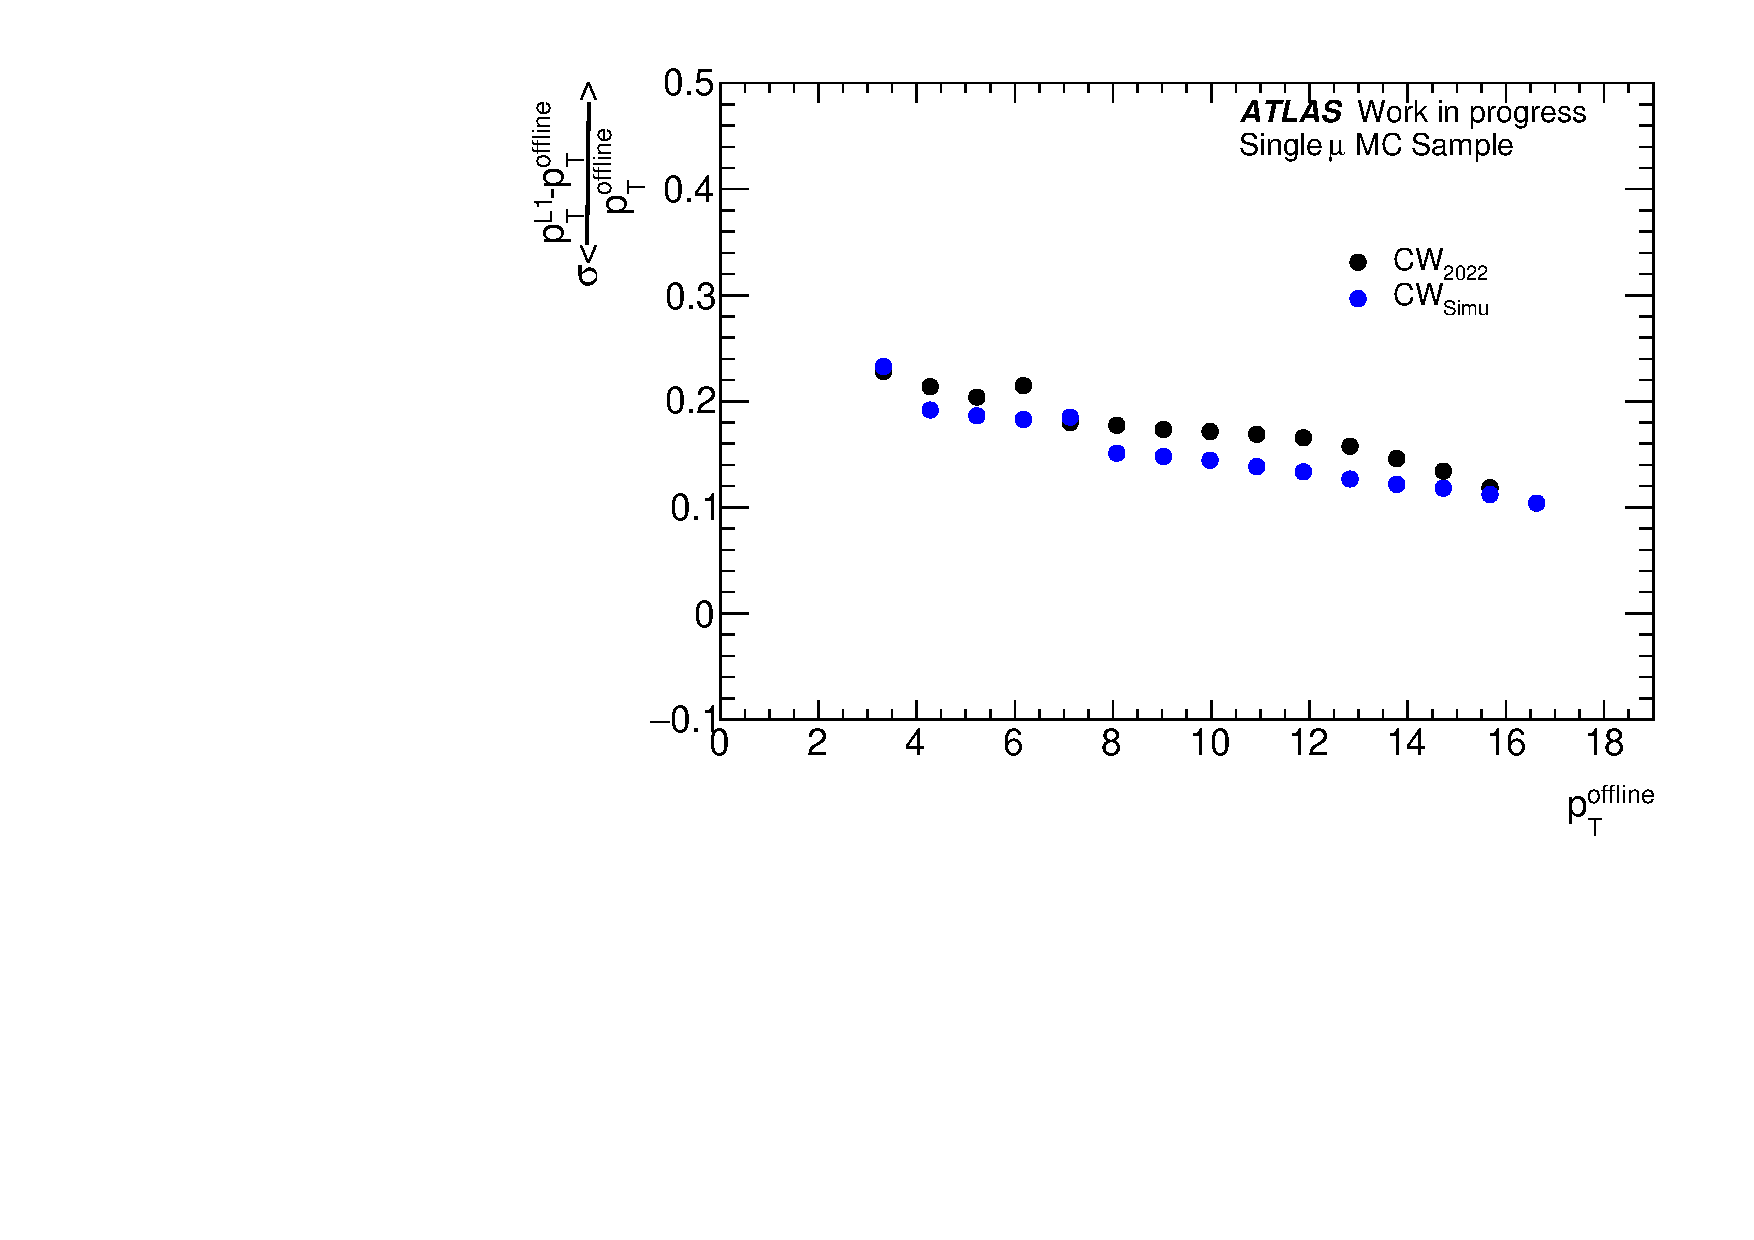
\includegraphics[clip, width=8cm]{fig/5/residual_stdDeVpdf_MC.pdf}
        %\vspace{5pt}
        \subcaption{標準偏差}
        \label{fig:resi_std_Simu}
    \end{minipage}
    \end{tabular}
    \caption{本研究の手法で作成した$\mathrm{CW_{Simu}}$と2022年度Run-2で使用された$\mathrm{CW_{2022}}$の$p_{\rm{T}}$ residualの比較。}
    \label{residual_MC}
\end{figure}

同様にして、本研究の手法で作成した$\mathrm{CW_{Data}}$と2022年度Run-2で使用された$\mathrm{CW_{2022}}$の比較を行う。図~\ref{residual_Data_3_18}に1~GeVごとの$p_{\rm{T}}^{\rm{offline}}$に対する$p_{\rm{T}}$ residual分布を示し、図~\ref{residual_Data}には1GeV刻みの$p_{\rm{T}}$ residual分布のMean値と標準偏差を示す。
本研究の手法で作成した$\mathrm{CW_{Data}}$は、2022年度Run-2で使用された$\mathrm{CW_{2022}}$と比べて$p_{\rm{T}}^{\rm{offline}}$分解能のmean値が悪くなっているが、標準偏差を比べると改善されていることから、$\mathrm{CW_{Simu}}$の評価で述べたように、機械学習の出力からの$p_{\rm{T}}$閾値の選択方法によってmean値においても改善が見込まれる。
\begin{figure}[htbp]
  \centering
  %\rule{8cm}{6cm}
  \hspace*{-1cm}
  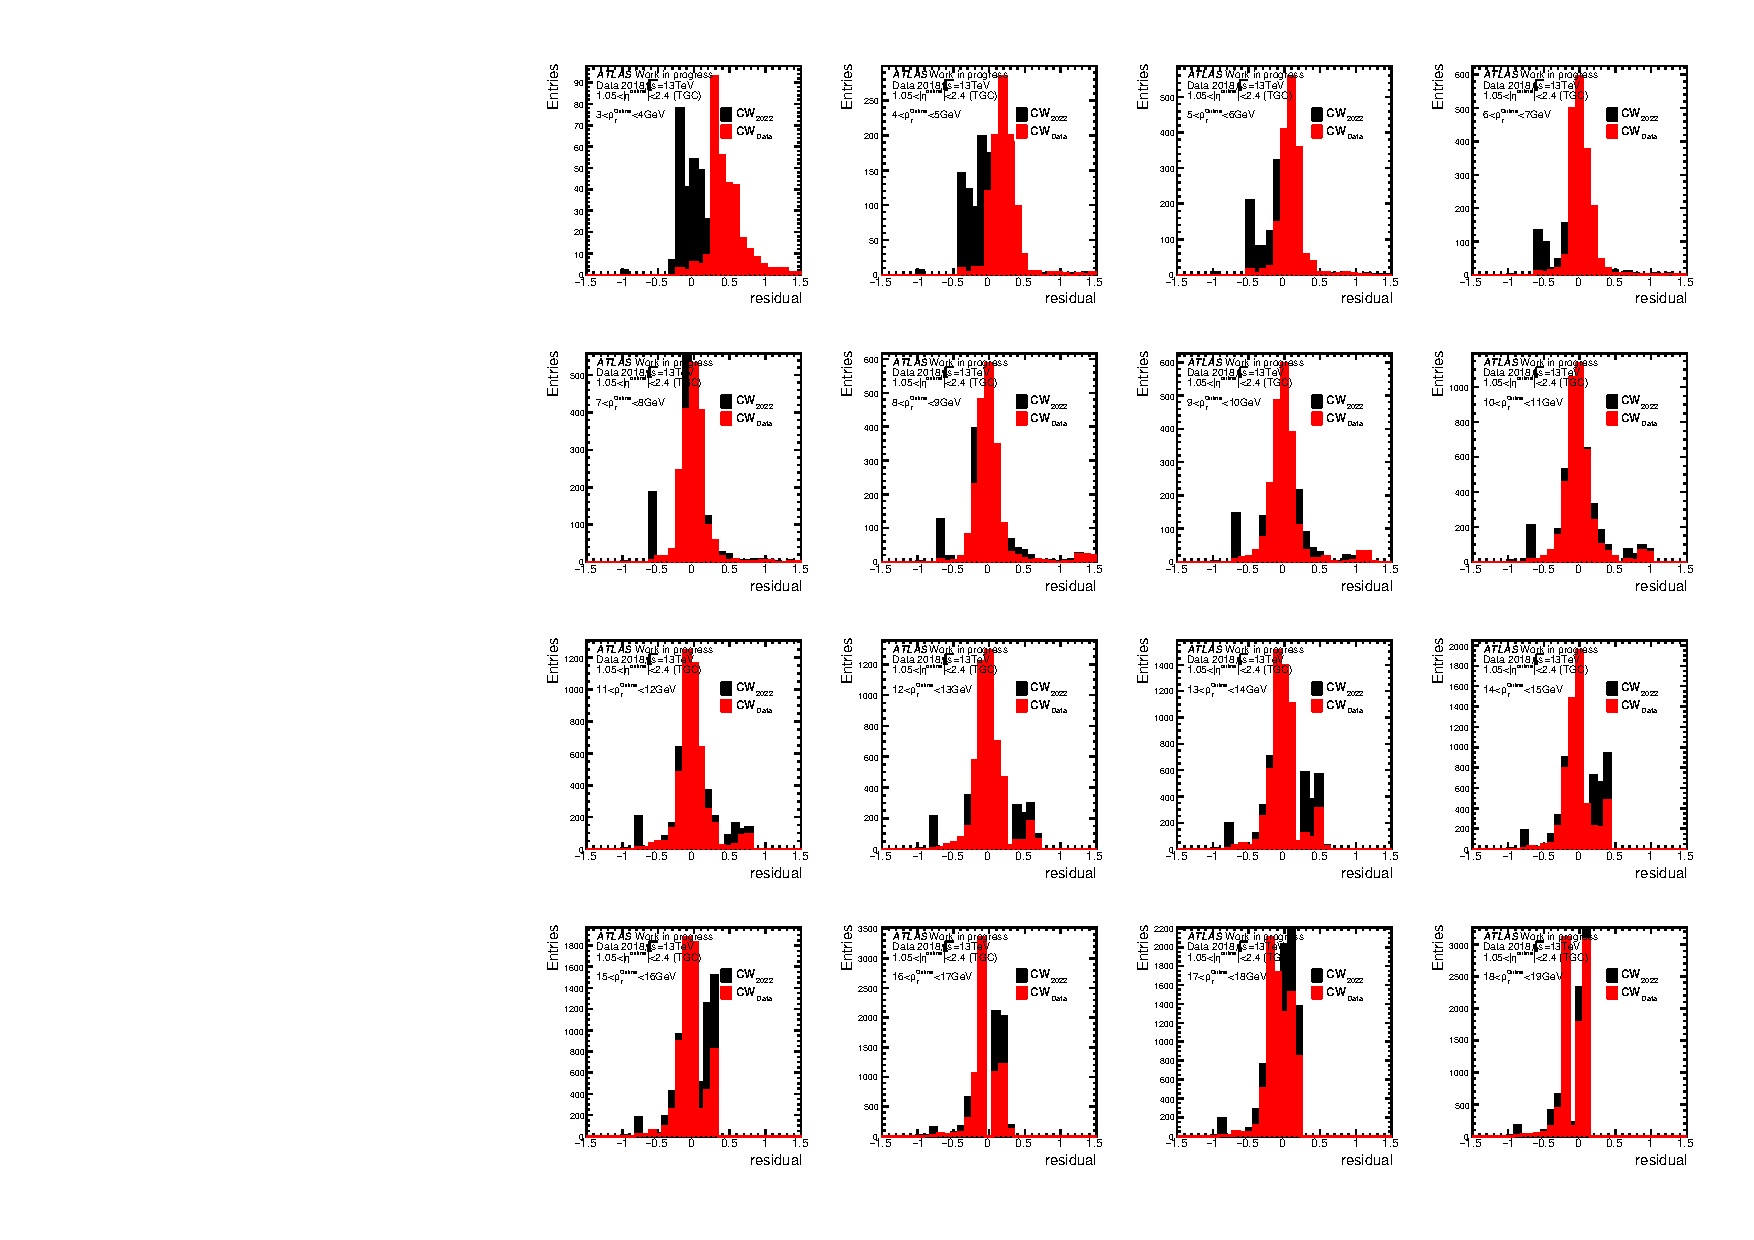
\includegraphics[clip, width=16cm]{fig/5/residual_Data_3_18.pdf}
  \caption{TGCにおける1GeV刻みのpT residual分布(3$\sim$18~GeV)。赤が本研究の手法で作成した$\mathrm{CW_{Data}}$を用いた結果、黒が2022年度Run-2で使用された$\mathrm{CW_{2022}}$を用いた結果である。}
  \label{residual_Data_3_18}
\end{figure}

%\begin{figure}[htb]
%  \centering
%  %\rule{8cm}{6cm}
%  \hspace*{-1cm}
%  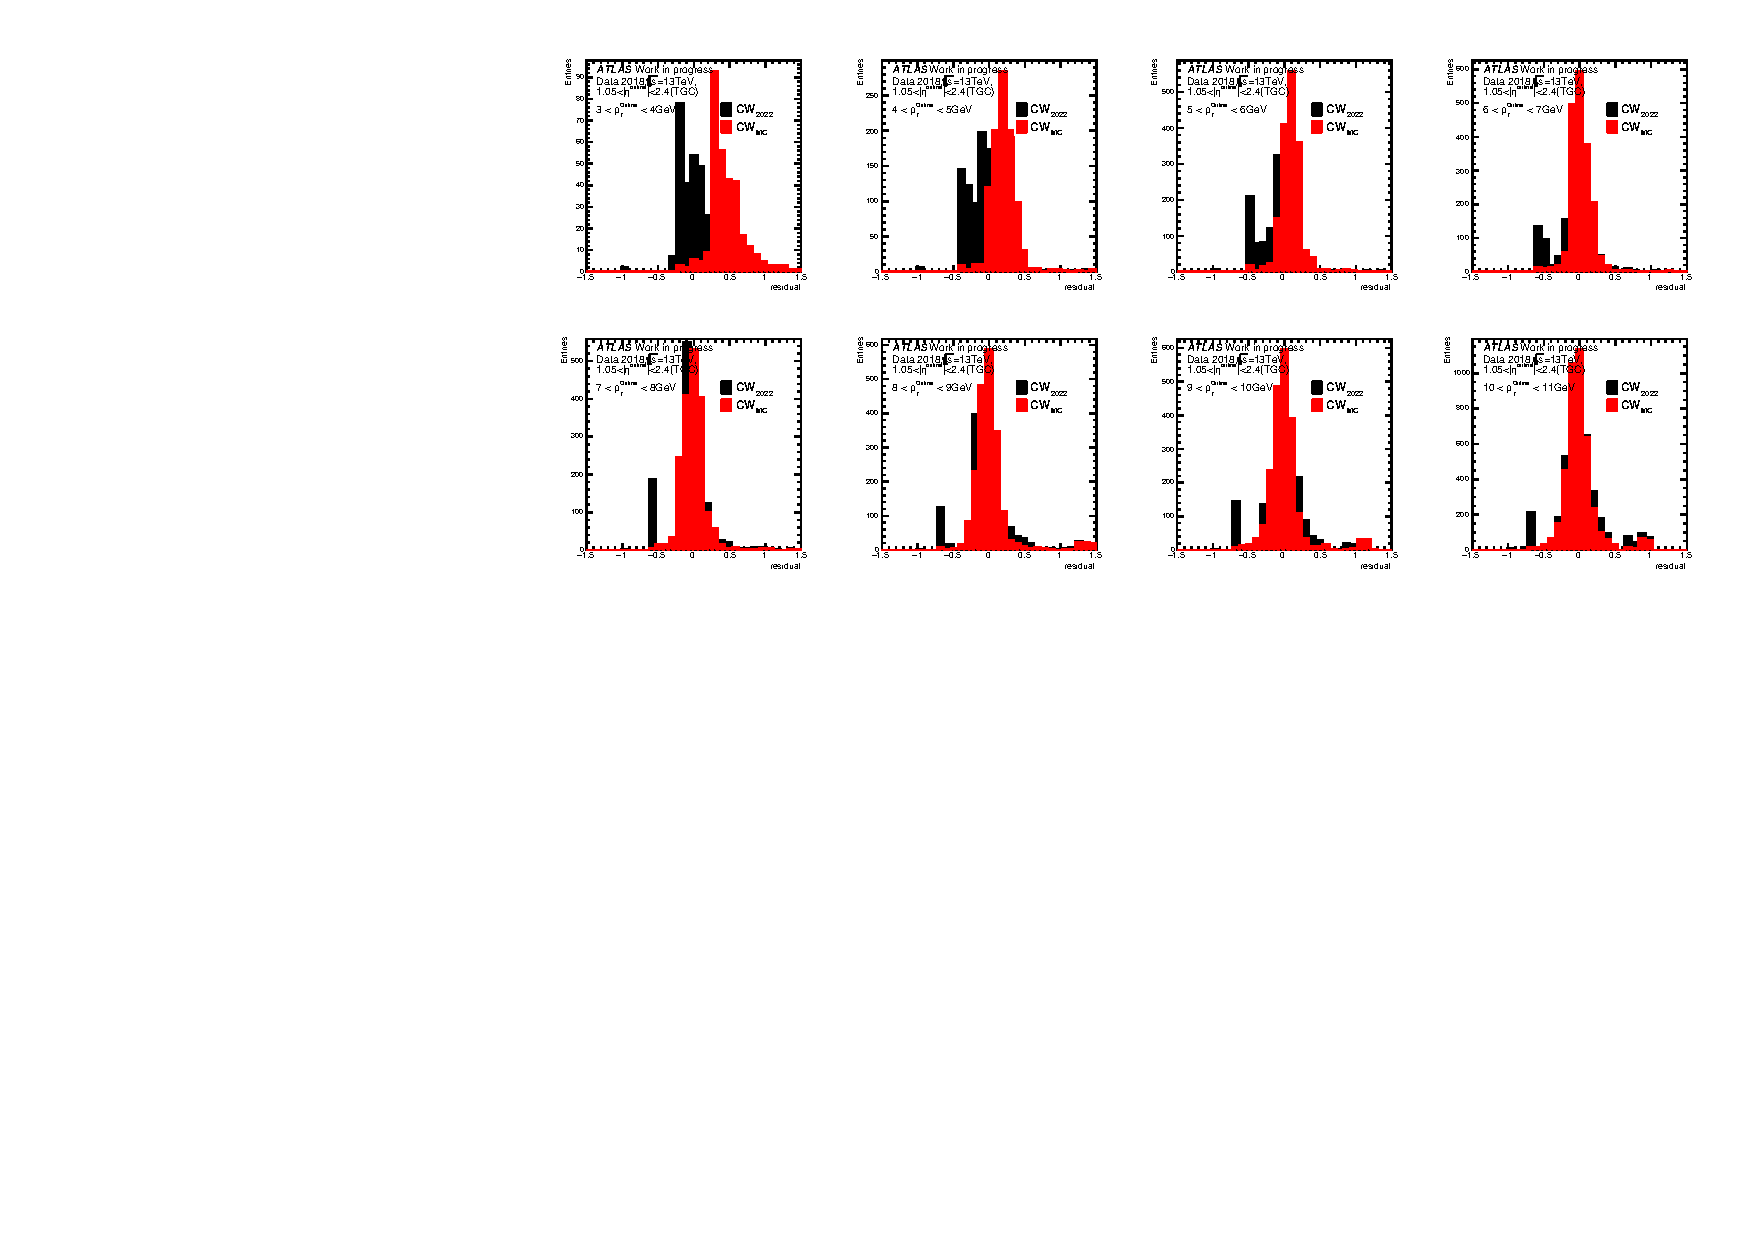
\includegraphics[clip, width=16cm]{fig/5/residual_Data_3_10.pdf}
%  \caption{TGCにおける1GeV刻みのpT residual分布(3$\sim$10~GeV)。赤が本研究の手法で作成した$\mathrm{CW_{Data}}$を用いた結果、黒が2022年度Run-2で使用された$\mathrm{CW_{2022}}$を用いた結果である。}
%  \label{residual_Data_3_10}
%\end{figure}
%\begin{figure}[htb]
%  \centering
%  %\rule{8cm}{6cm}
%  \hspace*{-1cm}
%  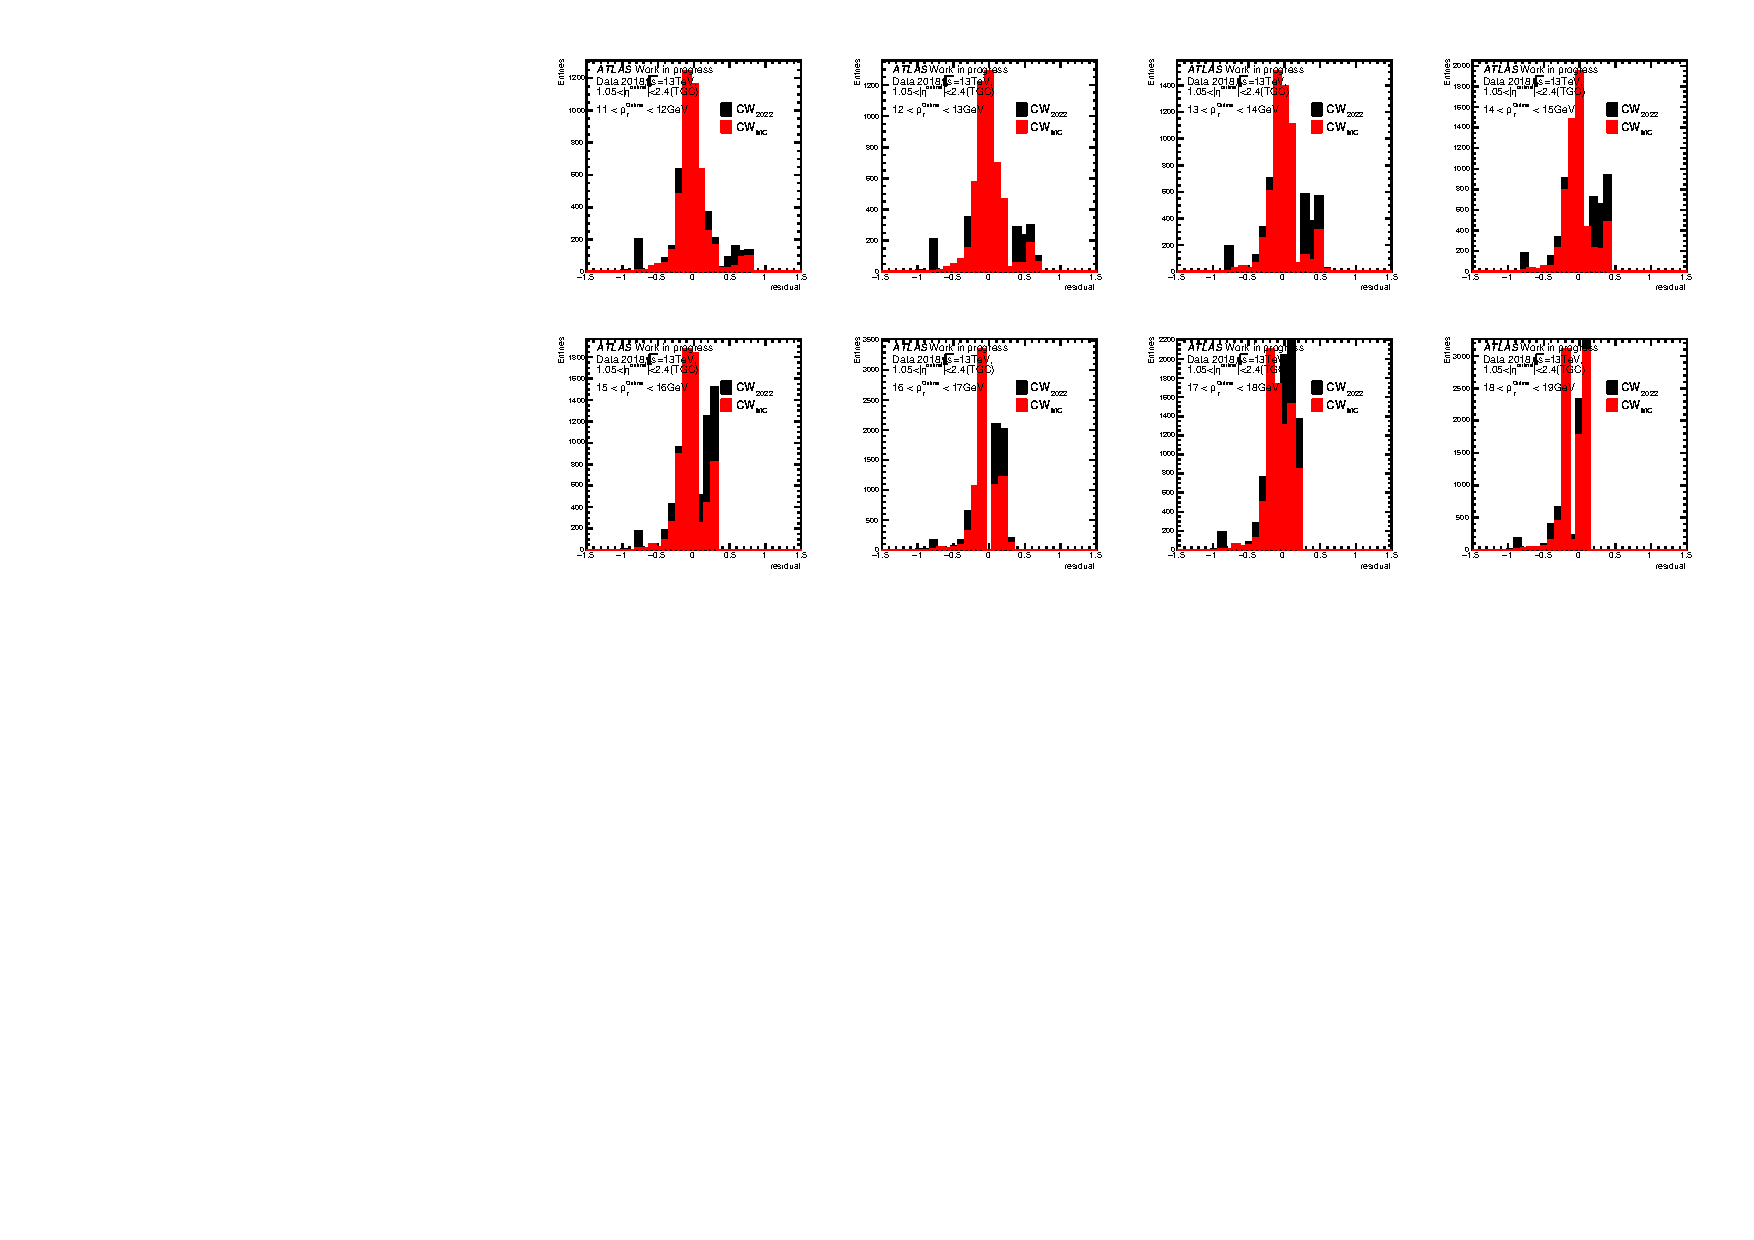
\includegraphics[clip, width=16cm]{fig/5/residual_Data_11_18.pdf}
%  \caption{TGCにおける1GeV刻みのpT residual分布(11$\sim$18~GeV)。赤が本研究の手法で作成した$\mathrm{CW_{Data}}$を用いた結果、黒が2022年度Run-2で使用された$\mathrm{CW_{2022}}$を用いた結果である。}
%  \label{residual_Data_11_18}
%\end{figure}



\begin{figure}
    %\centering
    \begin{tabular}{cc}
    \begin{minipage}[b]{0.45\hsize}
        %\centering
        \hspace*{-1cm}
        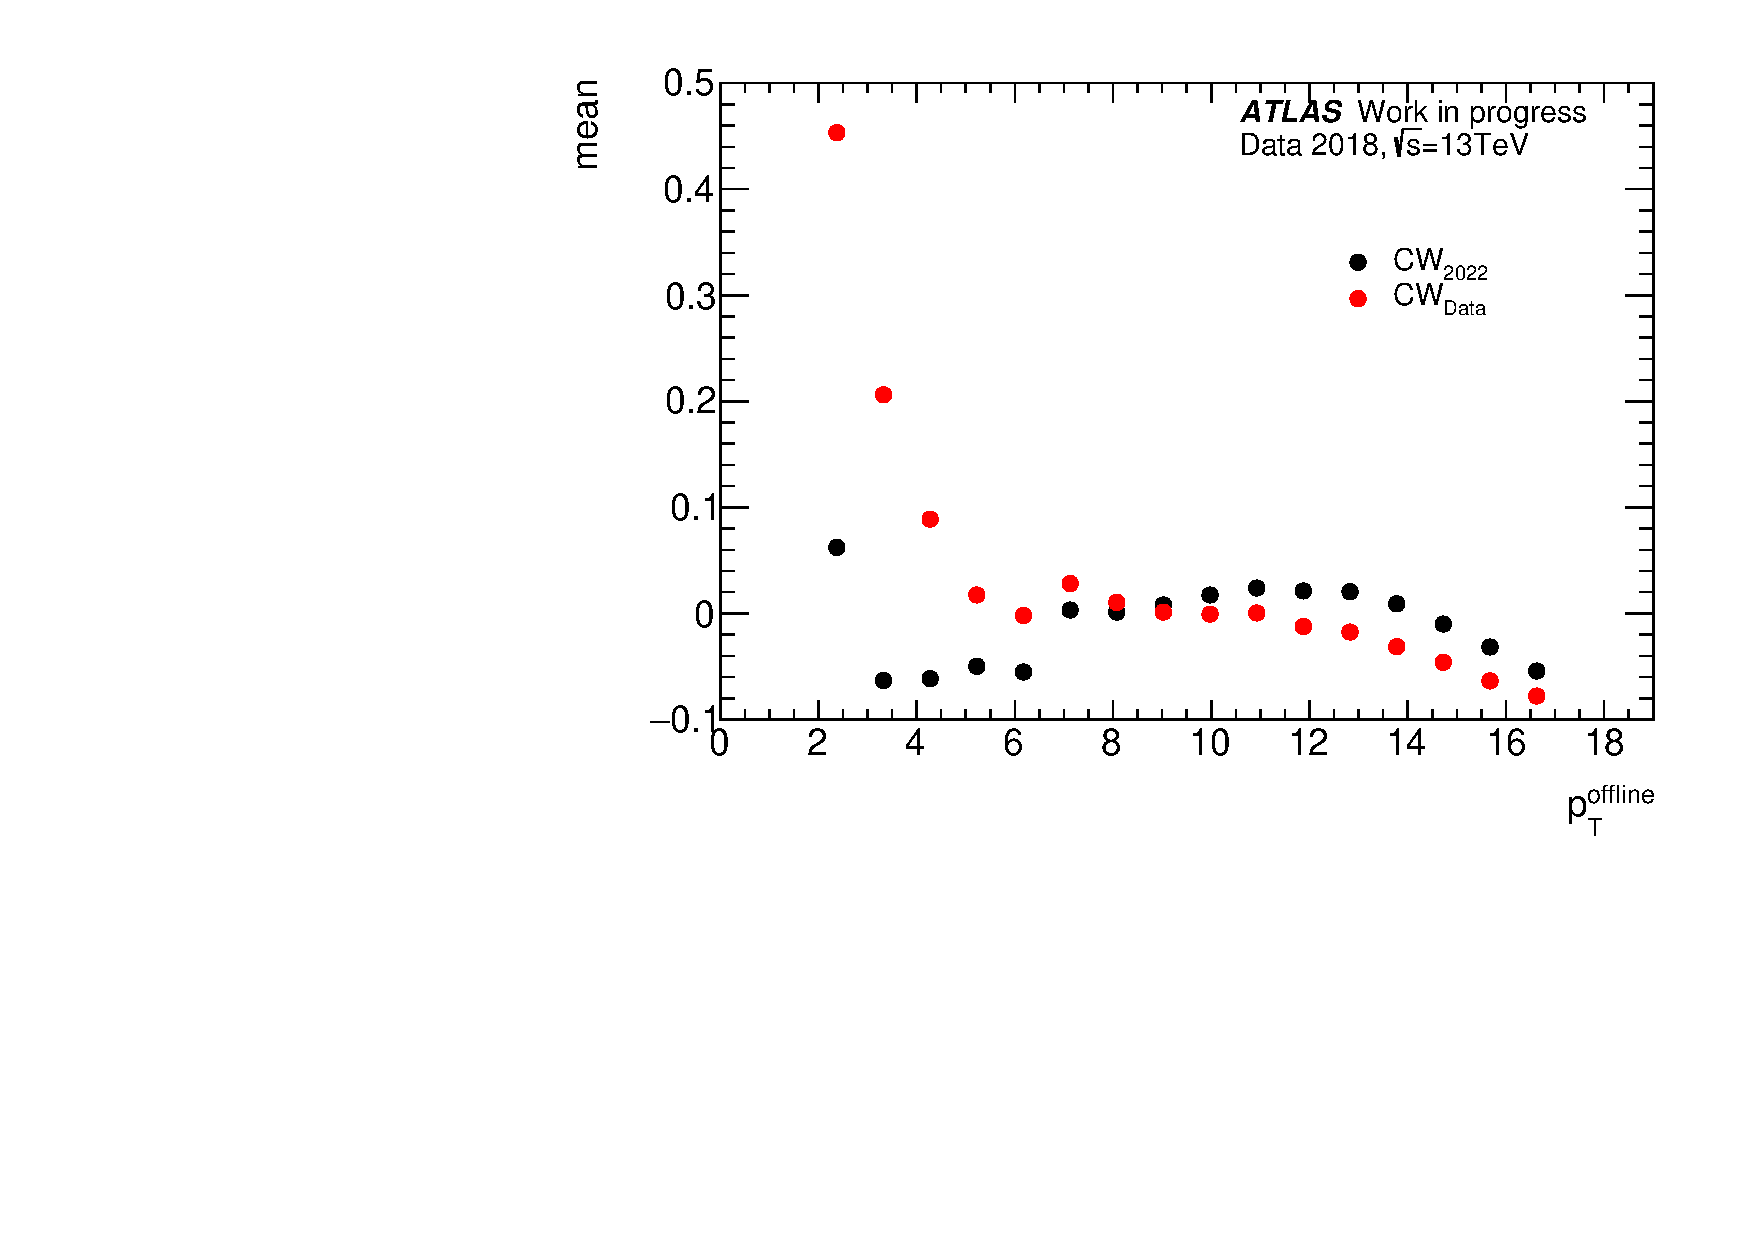
\includegraphics[clip, width=8cm]{fig/5/residual_mean_Data.pdf}
        %\vspace{5pt}
        \subcaption{Mean値}
        \label{fig:resi_mean_Data}
    \end{minipage}&
    %\hfill
    \begin{minipage}[b]{0.55\hsize}
        %\centering
        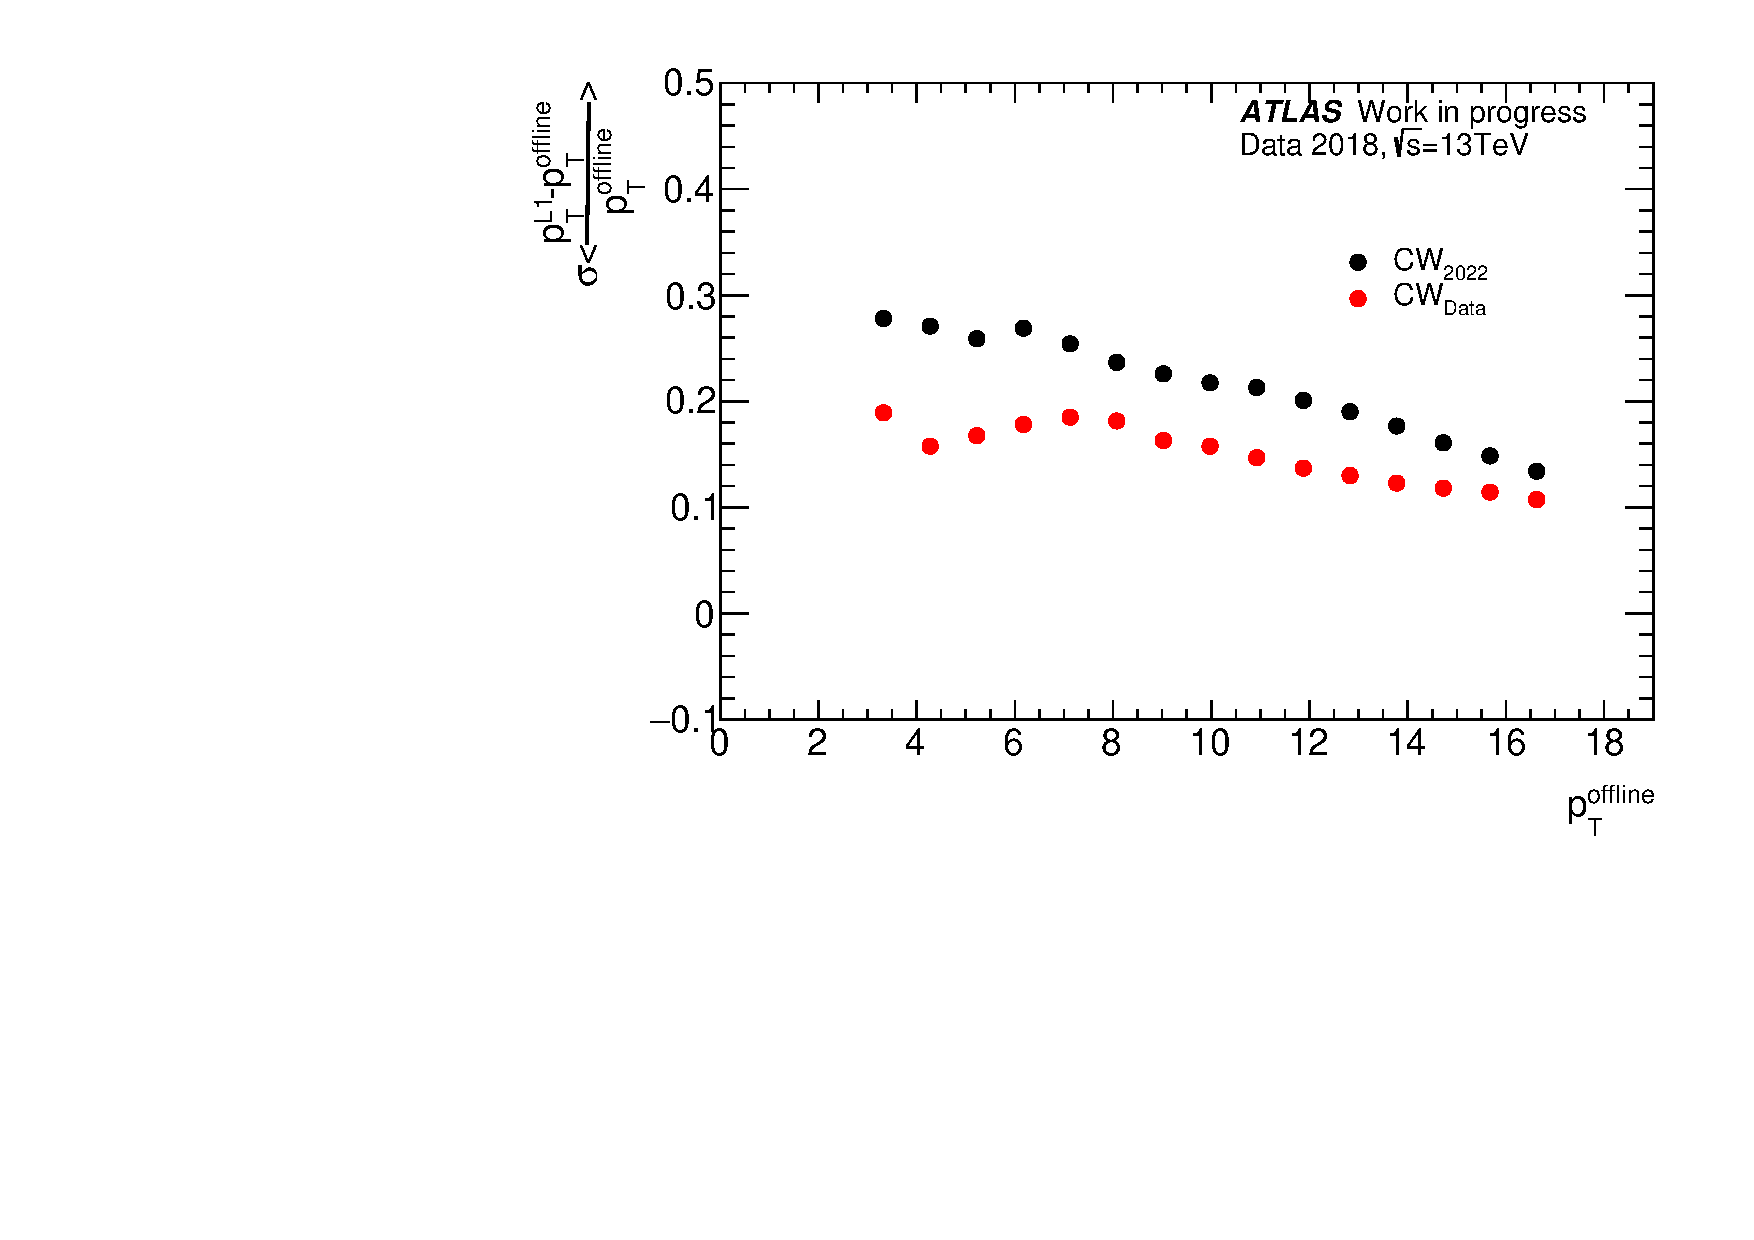
\includegraphics[clip, width=8cm]{fig/5/residual_stdDeVpdf.pdf}
        %\vspace{5pt}
        \subcaption{標準偏差}
        \label{fig:resi_std_Data}
    \end{minipage}
    \end{tabular}
    \caption{本研究の手法で作成した$\mathrm{CW_{Data}}$と2022年度Run-2で使用された$\mathrm{CW_{2022}}$の$p_{\rm{T}}$ residualの比較。}
    \label{residual_Data}
\end{figure}





\subsection{機械学習によるCWの最適化の評価}
次に、実際のデータを機械学習に用いることで期待されるCWの最適化の効果について評価を行う。

本研究で開発した手法では、実際のデータをトレーニング用いて$\mathrm{CW_{Data}}$を作成した。そのため、最適化を行っていない$\mathrm{CW_{2022}}$よりもトリガー性能が向上することが期待される。

%まず、検出器アライメントに対応して実際にCWを補正できているかを確認する。
%8回転対象の磁場構造において、同じ磁場構造となる場所に位置するRoIのCWについて、$p_{\rm{T}}$閾値が14~GeVとなる領域の$\mathrm{CW_{Data}}$と$\mathrm{CW_{2022}}$の比較を図~\ref{fig:CWv05v07}に示す。
%図~\ref{fig:CWv05v07}に示す8個のCWは、シミュレーション上では磁場構造が同じになるため、黒枠で表される$\mathrm{CW_{2022}}$はすべて同じ形である。しかし、\ref{ズレ}節で述べたように、実際の検出器のズレによって場所によって磁場構造が異なるため、本手法で作成した$\mathrm{CW_{Data}}$ではCWに数マス分のズレが生じていることが確認できる。
%\begin{figure}[tb]
%  \centering
%  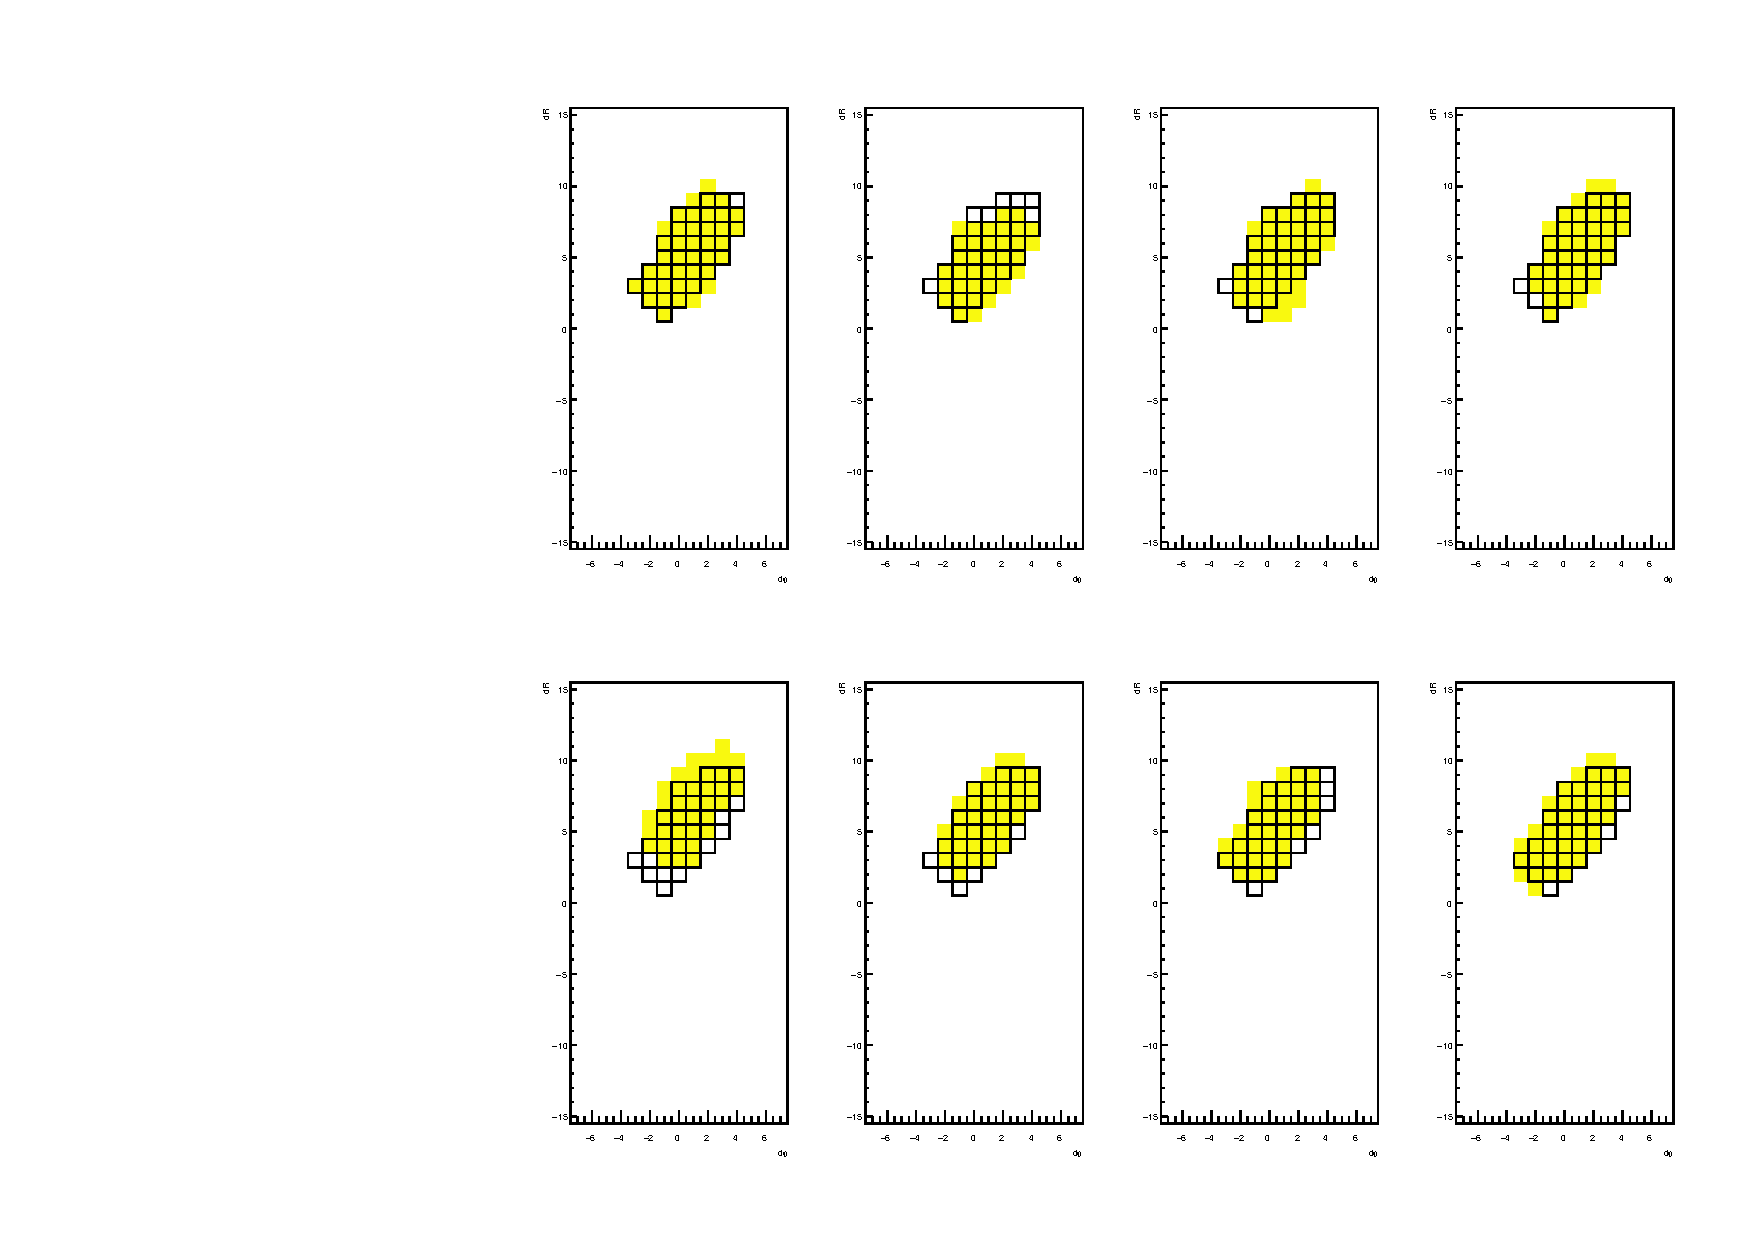
\includegraphics[clip, width=13cm]{fig/5/ALL_Aside_Endcap_phiSector_Octant1_roi58.pdf}
%  \caption{$p_{\rm{T}}$閾値が14~GeVとなる領域の比較。黄色の領域が本手法で作成した$\mathrm{CW_{Data}}$、黒枠の領域が$\mathrm{CW_{2022}}$である。}
%  \label{fig:CWv05v07}
%\end{figure}

まず、2018年Run-2データを評価に用いた時の、$\mathrm{CW_{Data}}$と$\mathrm{CW_{Simu}}$の性能の比較を行うことで、本研究の手法がトレーニングデータの違いを学習できているかを確認する。図~\ref{fig:v06v07}に$p_{\rm{T}}$閾値14~GeVにおけるTurn-on curveを比較したプロットを示す。最適化が行われた$\mathrm{CW_{Data}}$を用いたトリガーの方が、実際のデータに対してのトリガー効率が良くなっているのが見て取れる。
\begin{figure}[tb]
  \centering
  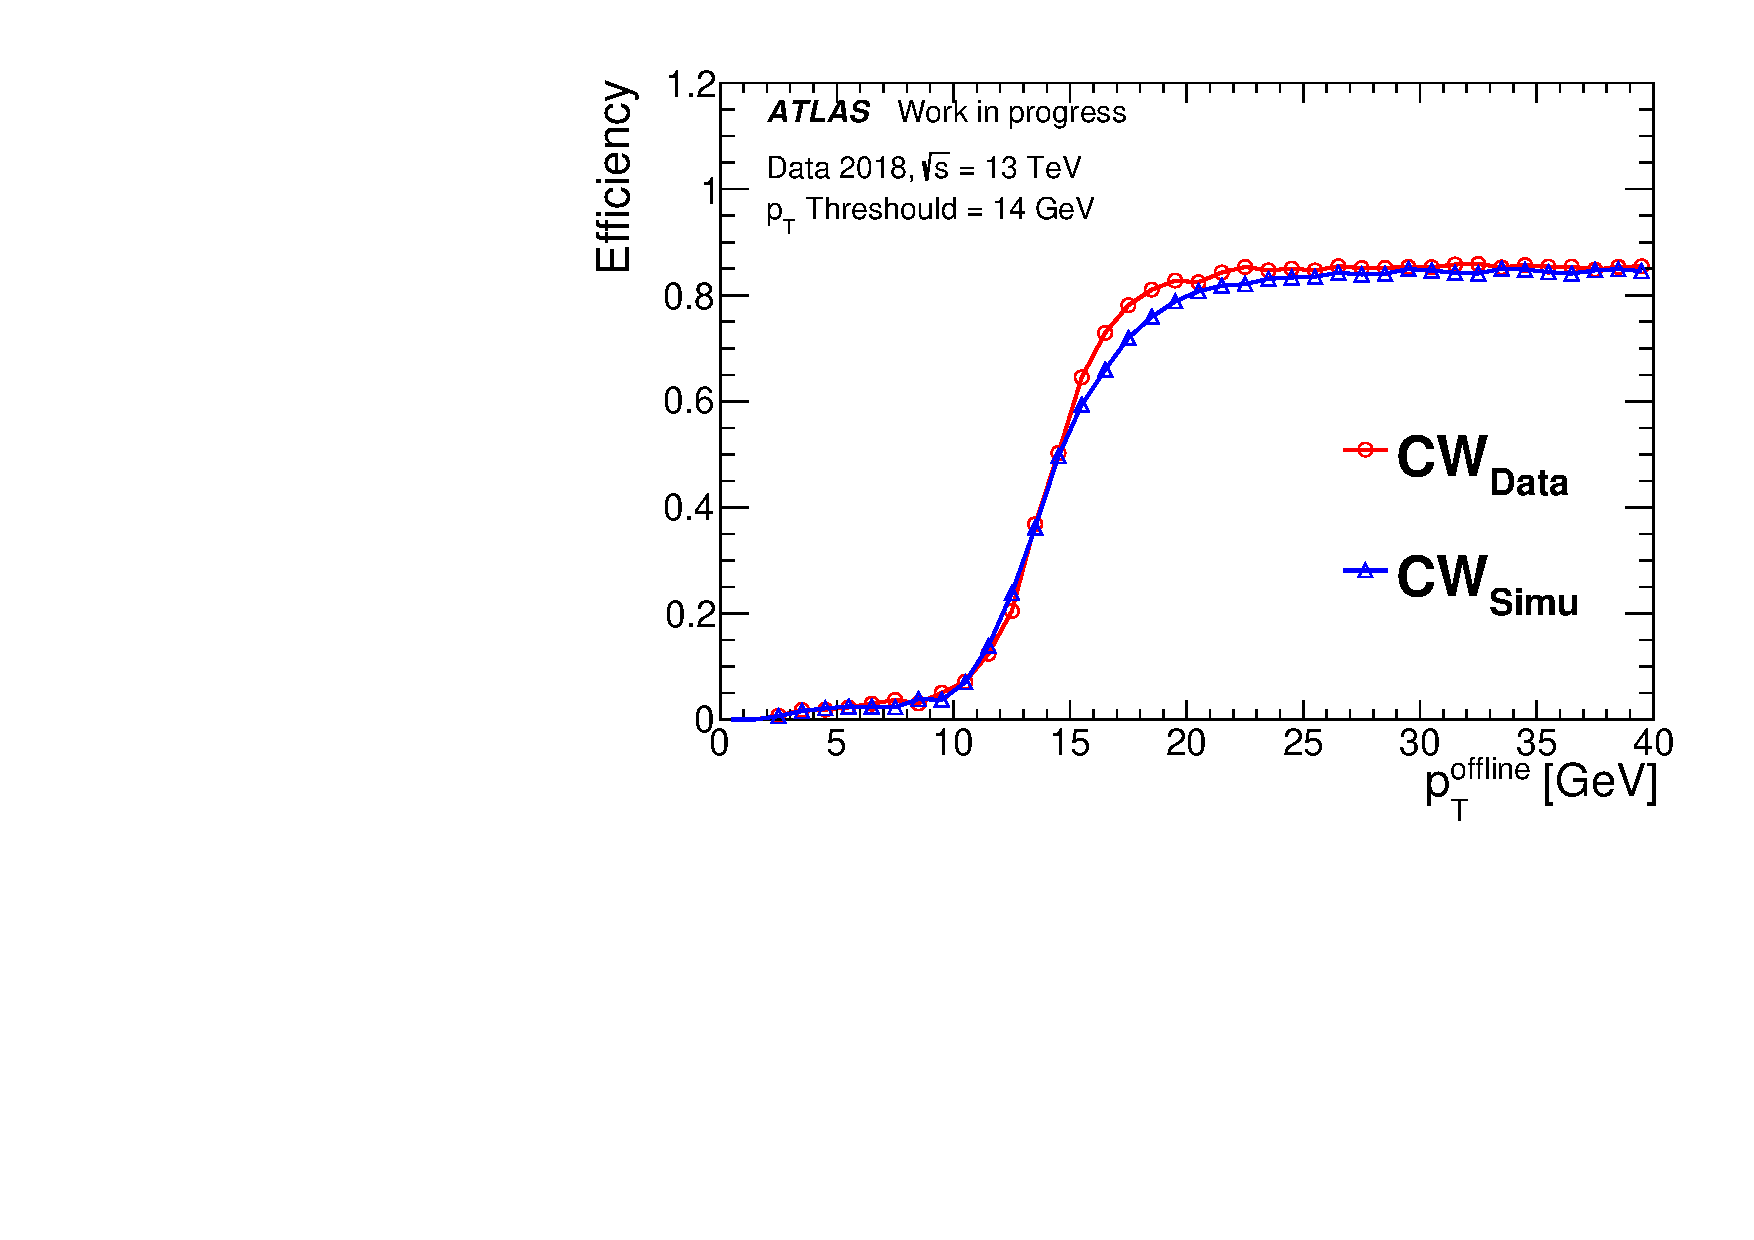
\includegraphics[clip, width=11cm]{fig/5/v06vsv07_MU14_re.pdf}
  \caption{$\mathrm{CW_{Data}}$と$\mathrm{CW_{Simu}}$のTurn-on curve。$p_{\rm{T}}$閾値14~GeVのトリガー効率の比較を行い、評価には2018年Run-2データを使用した。}
  \label{fig:v06v07}
\end{figure}

%\subsubsection{ミューオン電荷に対するトリガー性能の評価}
さらに、TGCチェンバーごとにミューオンの電荷別のトリガー効率の評価を行った。
あるTGCチェンバーにおける$\mathrm{CW_{Data}}$と$\mathrm{CW_{2022}}$の、ミューオンの電荷別に計算した$p_{\rm{T}}$閾値が14~GeVのトリガー効率を図~\ref{Eff_Chage}に示す。
検出器アライメントのズレがある場合、磁場中のミューオンは電荷によって曲がる方向が違うためトリガー判定に電荷依存が生じる。図~\ref{fig:v05_charge}に電荷別に計算したTurn-on curveを示す。$\mathrm{CW_{2022}}$は検出器のズレに対する補正を行っていないために、ミューオンの電荷別に計算したトリガー効率に大きな差が出ることが確認できる。
一方、本研究の手法で作成した$\mathrm{CW_{Data}}$はCWが最適化されたことにより、電荷別に計算したトリガー効率がほとんど一致していることが見て取れる。
\begin{figure}[htbp]
    %\centering
    \begin{tabular}{cc}
    \begin{minipage}[b]{0.45\hsize}
        %\centering
        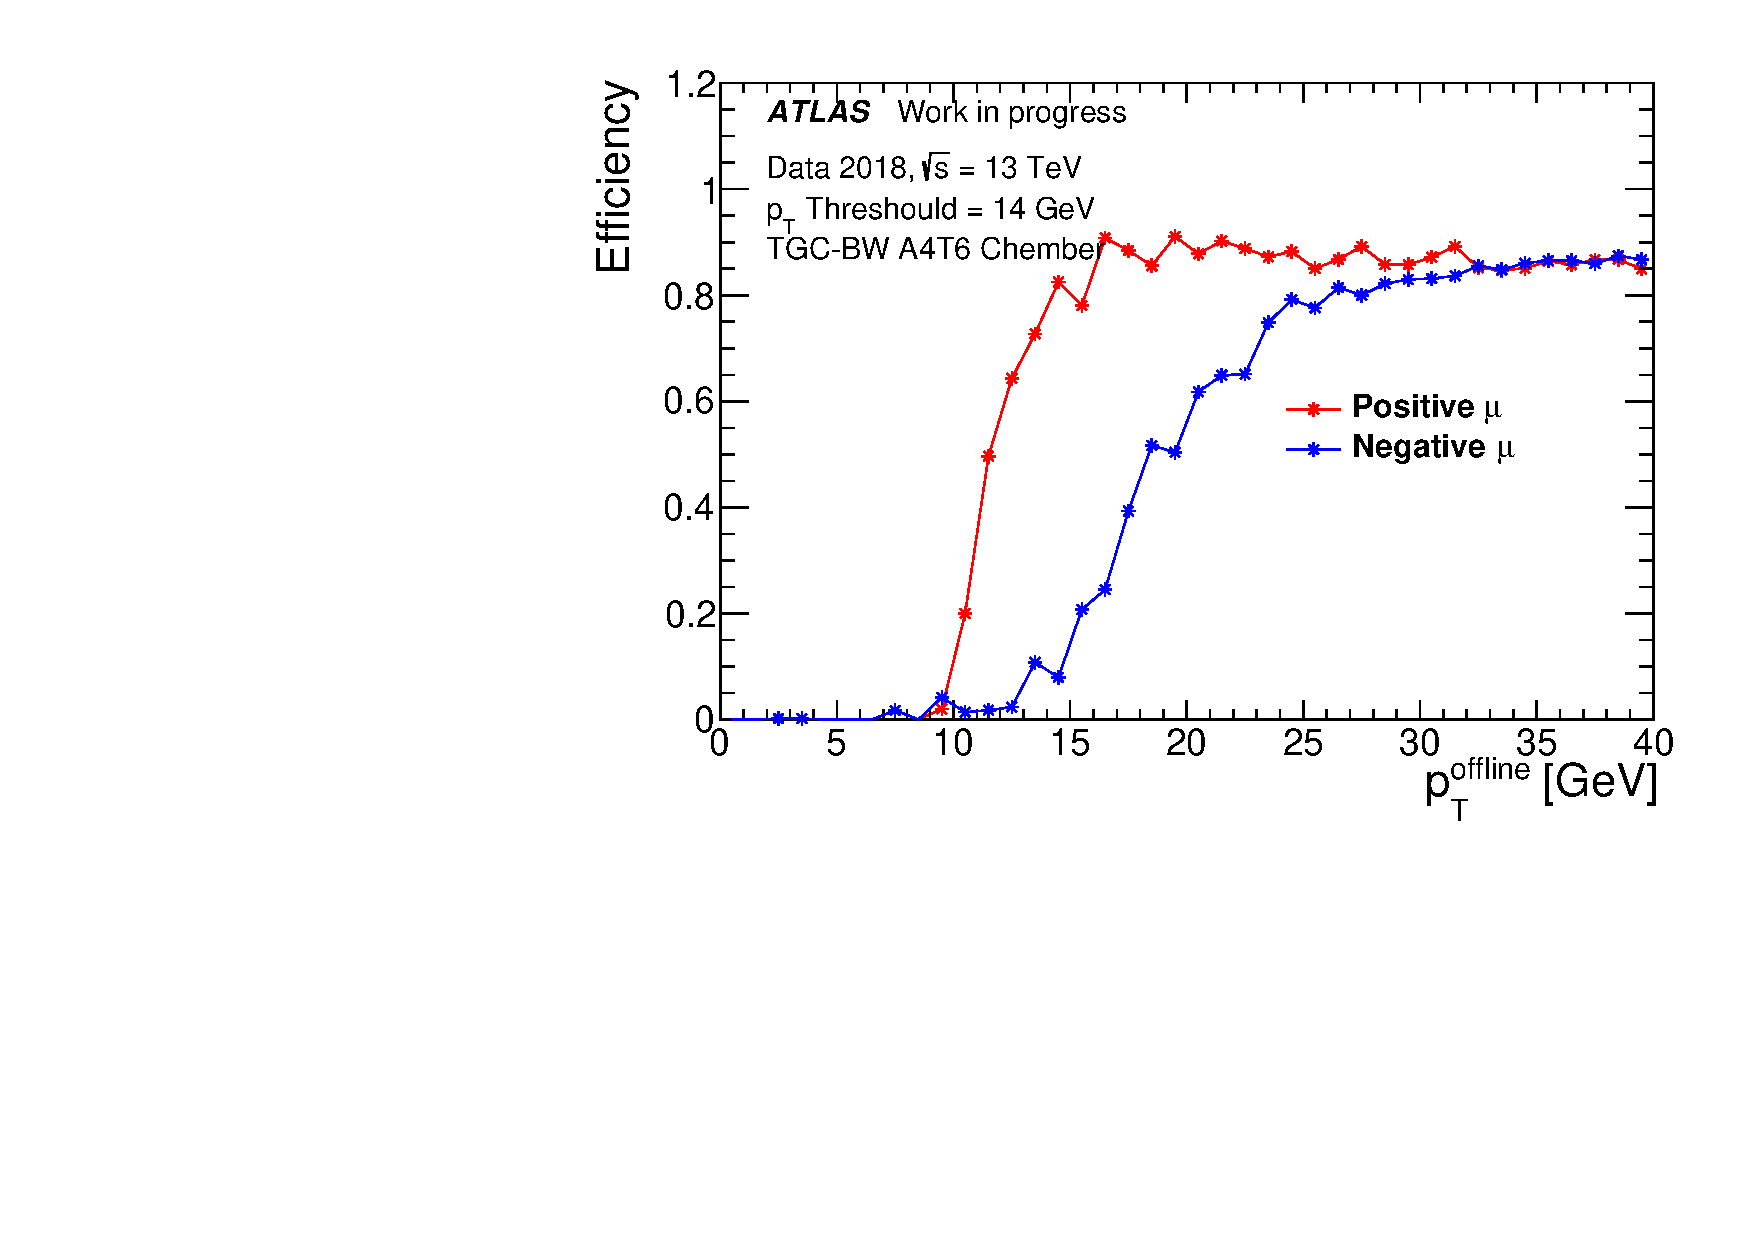
\includegraphics[clip, width=7cm]{fig/5/Eff_PNcharge_v05_phi0eta10_re.pdf}
        %\vspace{5pt}
        \subcaption{$\mathrm{CW_{2022}}$}
        \label{fig:v05_charge}
    \end{minipage}&
    %\hfill
    \begin{minipage}[b]{0.45\hsize}
        %\centering
        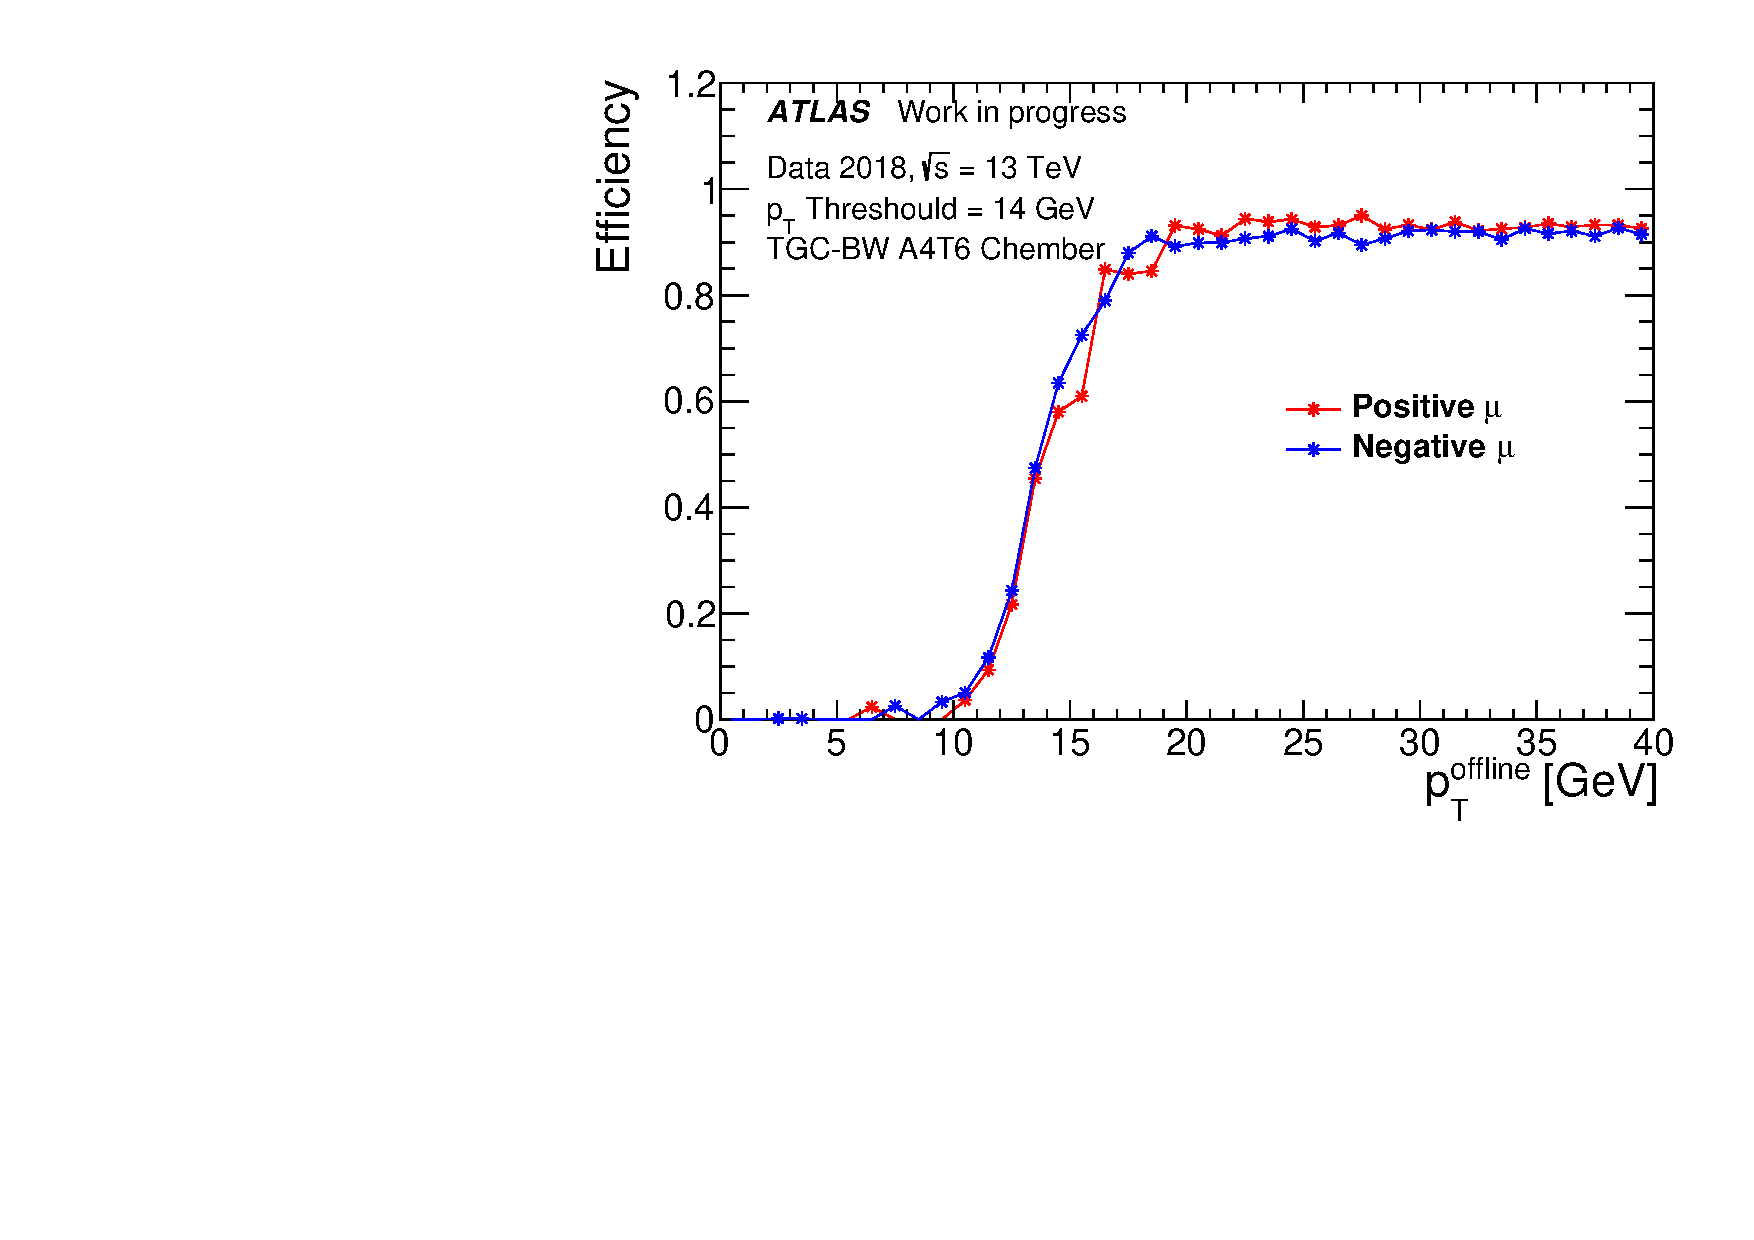
\includegraphics[clip, width=7cm]{fig/5/Eff_PNcharge_MLP_phi0eta10_re.pdf}
        %\vspace{5pt}
        \subcaption{$\mathrm{CW_{Data}}$}
        \label{fig:v06_charge}
    \end{minipage}
    \end{tabular}
    \caption{あるチェンバーにおける電荷別に計算した$p_{\rm{T}}$閾値14~GeVのTurn-on curveの比較。赤が正電荷、青が負電荷。}
    \label{Eff_Chage}
\end{figure}

本研究の手法では、実際のデータを機械学習のトレーニングに用いたことで、TGC 検出器の位置による磁場構造の違いや検出器のズレを自動で補正することができ、CWが最適化されたことを示している。




\subsection{トリガーレートの評価}
次に、本手法で作成したCWを使用したときのトリガーレートの評価を行う。トリガーレートとは、実験データにおけるトリガーが発行された事象数である。
2018年のRun-2データを用いてトリガーレートを計算する。
Run-2データにはHLTでのプリスケールによるバイアスが存在するため、バイアスのない状態でトリガーレートを計算するために、「HLT$\_$noalg$\_$L1MU4」を要求する。このトリガーはL1トリガーにおいて$p_{\rm{T}}$閾値が4GeV以上を要求するが、HLTによる事象選別のない(Passthrough)トリガーチェインである。
その後、HLT$\_$noalg$\_$L1MU4が鳴ったイベントの中でL1$\_$MU$x$が鳴ったイベントがいくら存在するかを調べ、ルミノシティが$2\times10^{43}$~cm$^{-2}$s$^{-1}$の時のL1$\_$MU4のトリガーレート(3400~kHz)をかけることでMU$x$のトリガーレートを見積もる。式~\eqref{equ:トリガーレート}にトリガーレートの計算式を示す。
\begin{equation}
    \rm{MU}xのレート[\rm{kHz}] = \frac{\rm{MU}xが鳴ったイベント数}{HLT\_noalg\_L1MU4が鳴った全イベント数}\times L1\_MU4のレート[kHz]
    \label{equ:トリガーレート}
\end{equation}
図~\ref{fig:Ratev05v06}に2016年で取得されたデータを用いて算出したトリガーレートを示す。

\begin{figure}[tb]
  \centering
  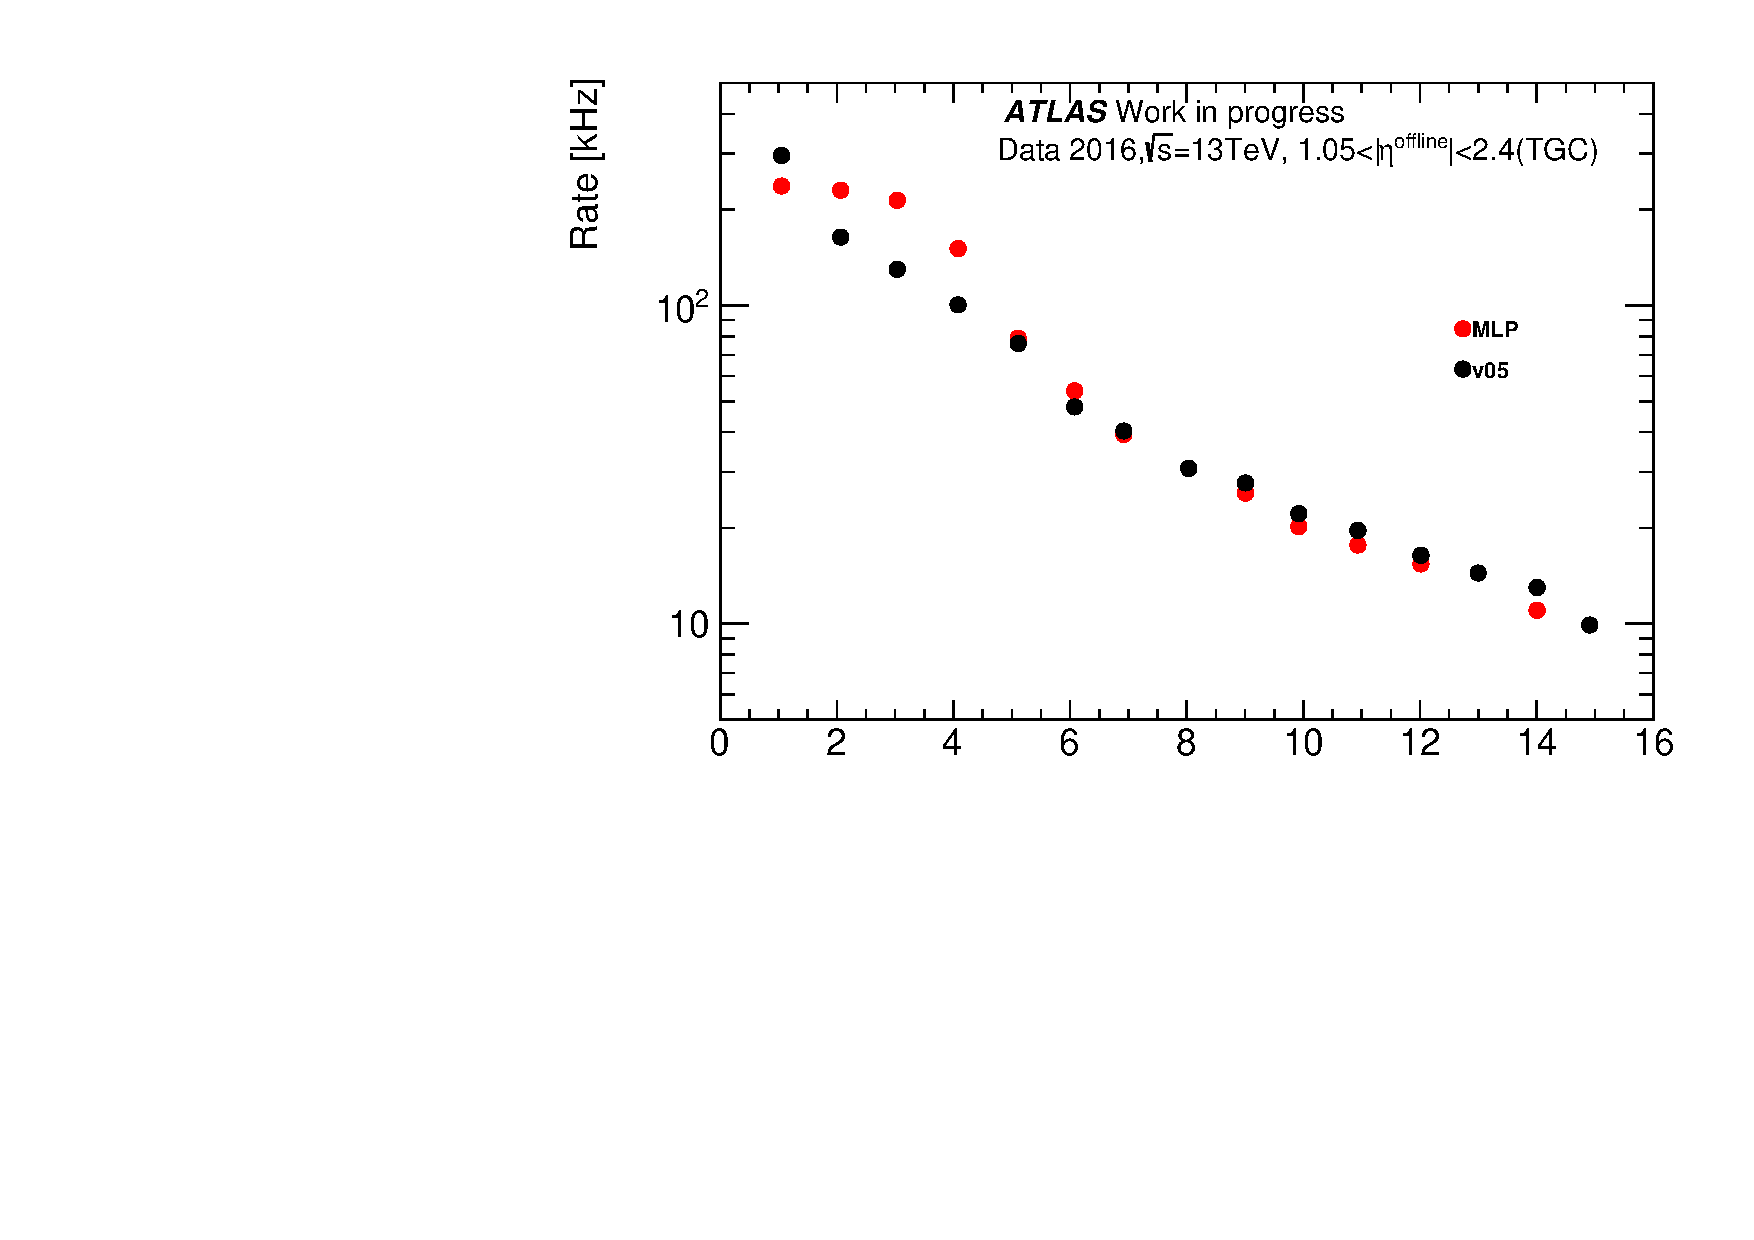
\includegraphics[clip, width=11cm]{fig/5/15rate.pdf}
  \caption{TGCにおけるシングルミューオンのトリガーレート。}
  \label{fig:Ratev05v06}
\end{figure}
プライマリートリガーである$p_{\rm{T}}$閾値14~GeVのトリガーレートは、本研究の手法で作成した$\mathrm{CW_{Data}}$では15~kHz、2022年度Run-2で使用された$\mathrm{CW_{2022}}$では16~kHzとなり、トリガーレートの削減が確認できた。また、$p_{\rm{T}}$閾値7~GeV以上のトリガーにおいて、$\mathrm{CW_{Data}}$のトリガーレートの値は$\mathrm{CW_{2022}}$と同等であることが見て取れる。
しかし、$p_{\rm{T}}$閾値4~GeV、5~GeV、6~GeVのトリガーに関してはトリガーレートの増加が見られた。
これは、\ref{fig:Effictive_thr_v1}で示したように、低いEffective Threshouldへの変換ができていなことが原因で、低い$p_{\rm{T}}$閾値のトリガーの性能が悪くなってしまったと思われる。
ただし、Run-3以降のエンドキャップ部のミューオントリガーでは\ref{section2-2-4}節で述べたようにNSWによるインナーコインシデンスが可能となり、トリガーレートの大幅な削減が見込まれている。そのため、本研究で作成したCWに対してもインナーコインシデンスを用いることで、$p_{\rm{T}}$閾値4~GeV、5~GeV、6~GeVのトリガーに関してもトリガーレートの削減が可能である。
また、本研究で開発した手法では、$p_{\rm{T}}$閾値を柔軟に選択することができるため、トリガーレートの削減に焦点を置いた$p_{\rm{T}}$閾値の選択をすることでトリガーレートを抑えることのできるCWを作成可能である。



\section{性能評価のまとめ}
本章では作成したCWの評価を行った。
15段階のトリガー効率の評価を、Turn-on CurveのPlateau EfficiencyとResolutionといった観点から評価を行っ結果、
本研究の手法で作成した2種類のCWは$\mathrm{CW_{2022}}$のTurn-on Curveと比べトリガー効率の向上が確認できた。
これは、検出器アライメントの最適化を行うことができていることを示している。
また、L1Muonのプライマリートリガーである$p_{\rm{T}}$閾値14~GeVのトリガー効率について、$\mathrm{CW_{2022}}$はトリガー効率が85.4$\%$であったのに対し、$\mathrm{CW_{Data}}$ではトリガー効率が86.7$\%$となったことから約1$\%$の向上が確認できた。

さらに、$p_{\rm{T}}$分解能の評価を$p_{\rm{T}}$ residualを計算することで評価を行った。
本研究の手法で作成したCWは、2022年度Run-2で使用された$\mathrm{CW_{2022}}$と比べて$p_{\rm{T}}^{\rm{offline}}$分解能のmean値が悪くなっているが、Resolutionを比べると改善されていることから、機械学習の出力からの$p_{\rm{T}}$閾値の選択方法を変更することによってmean値においても改善が見込まれる。

また、本研究の手法で期待される機械学習による最適化の評価を行った。
ミューオンの電荷別にトリガー効率を算出したところ、トリガー効率の電荷の依存性が見られなくなった。
このことから、検出器アライメントの最適化が行えていることが確認できた。

トリガーレートに関して、プライマリートリガーである$p_{\rm{T}}$閾値14~GeVのトリガーレートは、本研究の手法で作成した$\mathrm{CW_{Data}}$では約15~kHz、2022年度Run-2で使用された$\mathrm{CW_{2022}}$では約16~kHzとなり、トリガーレートの削減が確認できた。また、$p_{\rm{T}}$閾値7~GeV以上のトリガーにおいて、$\mathrm{CW_{Data}}$のトリガーレートの値は$\mathrm{CW_{2022}}$と同等であることが見て取れる。

以上より、本研究の手法である機械学習を用いた手法は、従来の手法と同様に15段階の閾値を持ったCWの作成を可能とし、さらに検出器アライメントに対する補正を自動的に行うことができることを示した。


本研究の手法では将来、検出器やシステムのアップグレードが行われた際に本研究の手法が有効である。
実際のデータ

%\begin{figure}[htbp]
%    %\centering
%    \begin{tabular}{cc}
%    \begin{minipage}[b]{0.45\hsize}%
%        %\centering
%        \hspace*{-1cm}
%        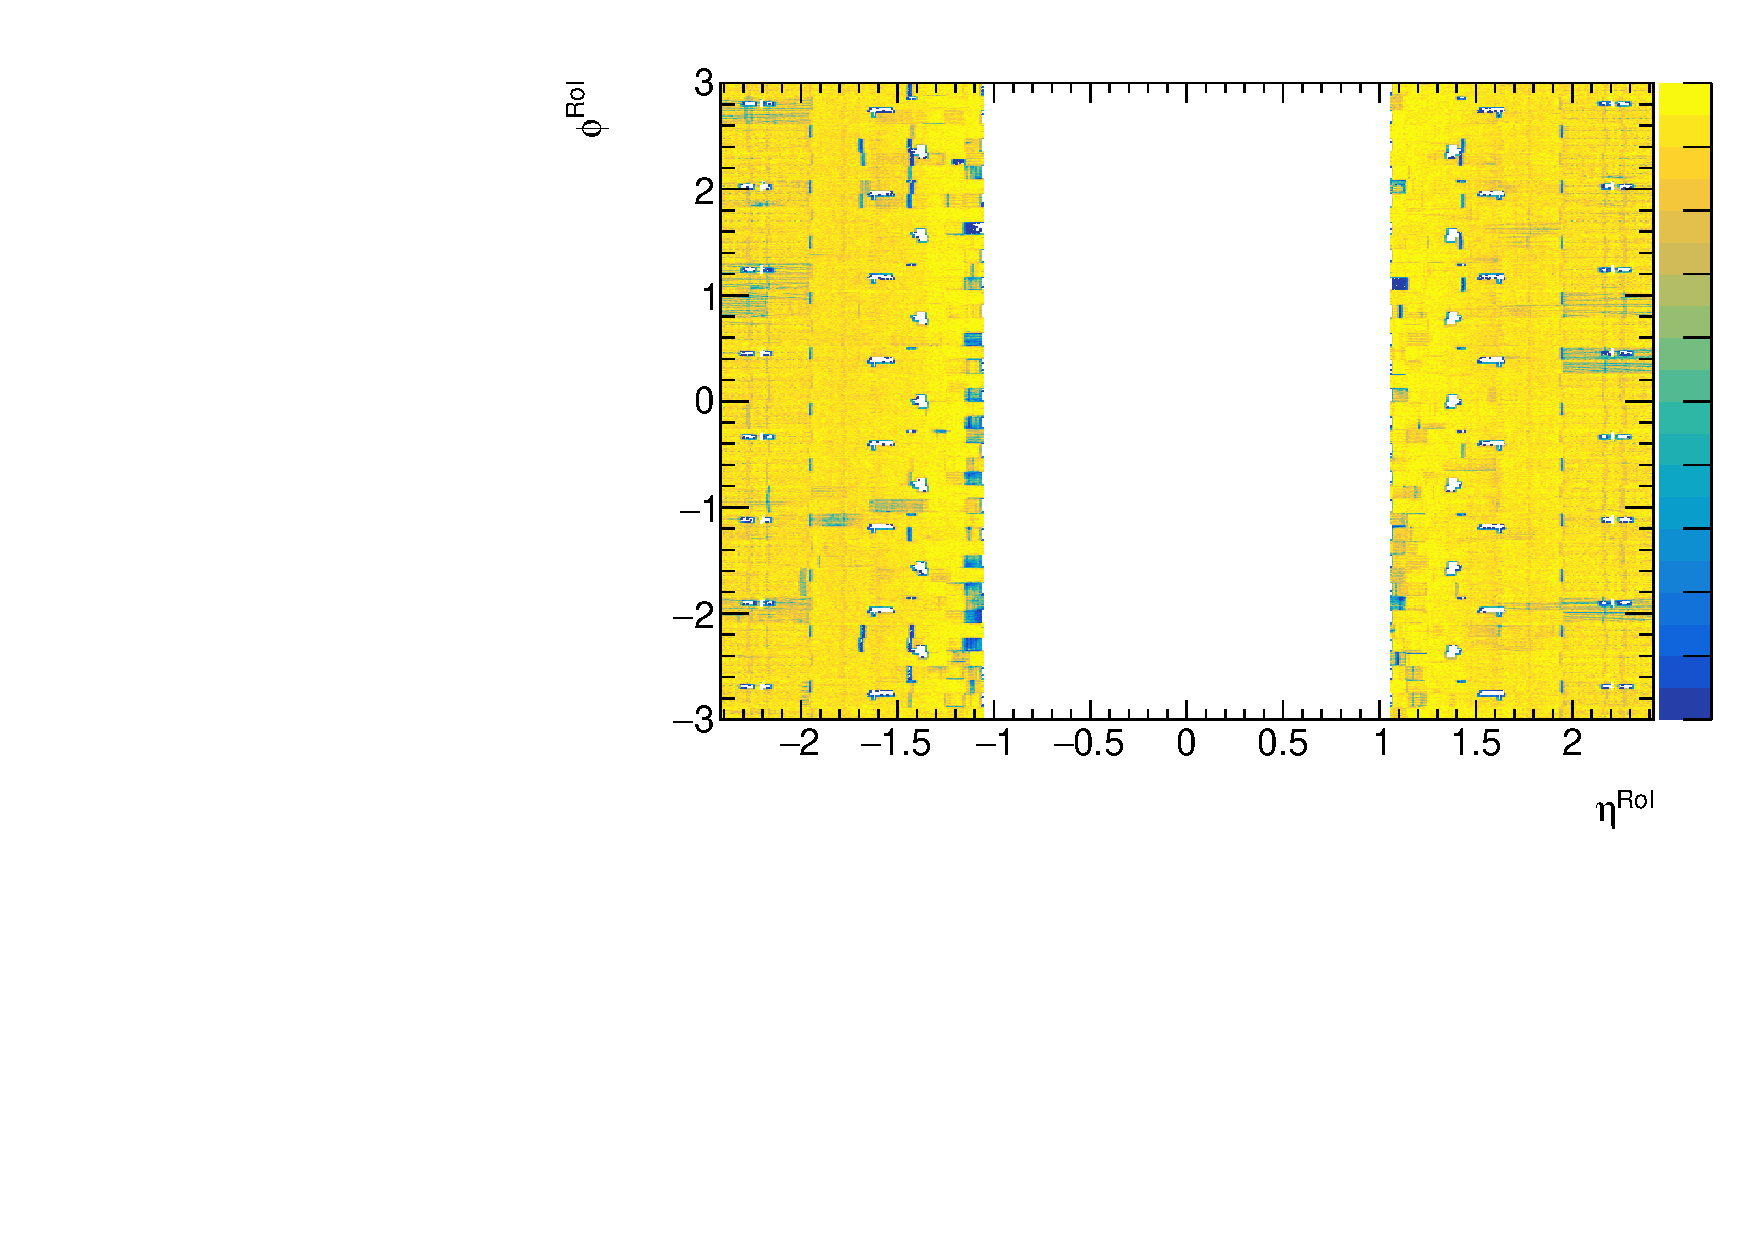
\includegraphics[clip, width=7cm]{fig/5/h2_Data14_Eff.pdf}
%        %\vspace{5pt}
%        \subcaption{}
%        \label{fig:dataEffMU14}
%    \end{minipage}%
%    %\hfill
%    \begin{minipage}[b]{0.55\hsize}%
%        %\centering
%        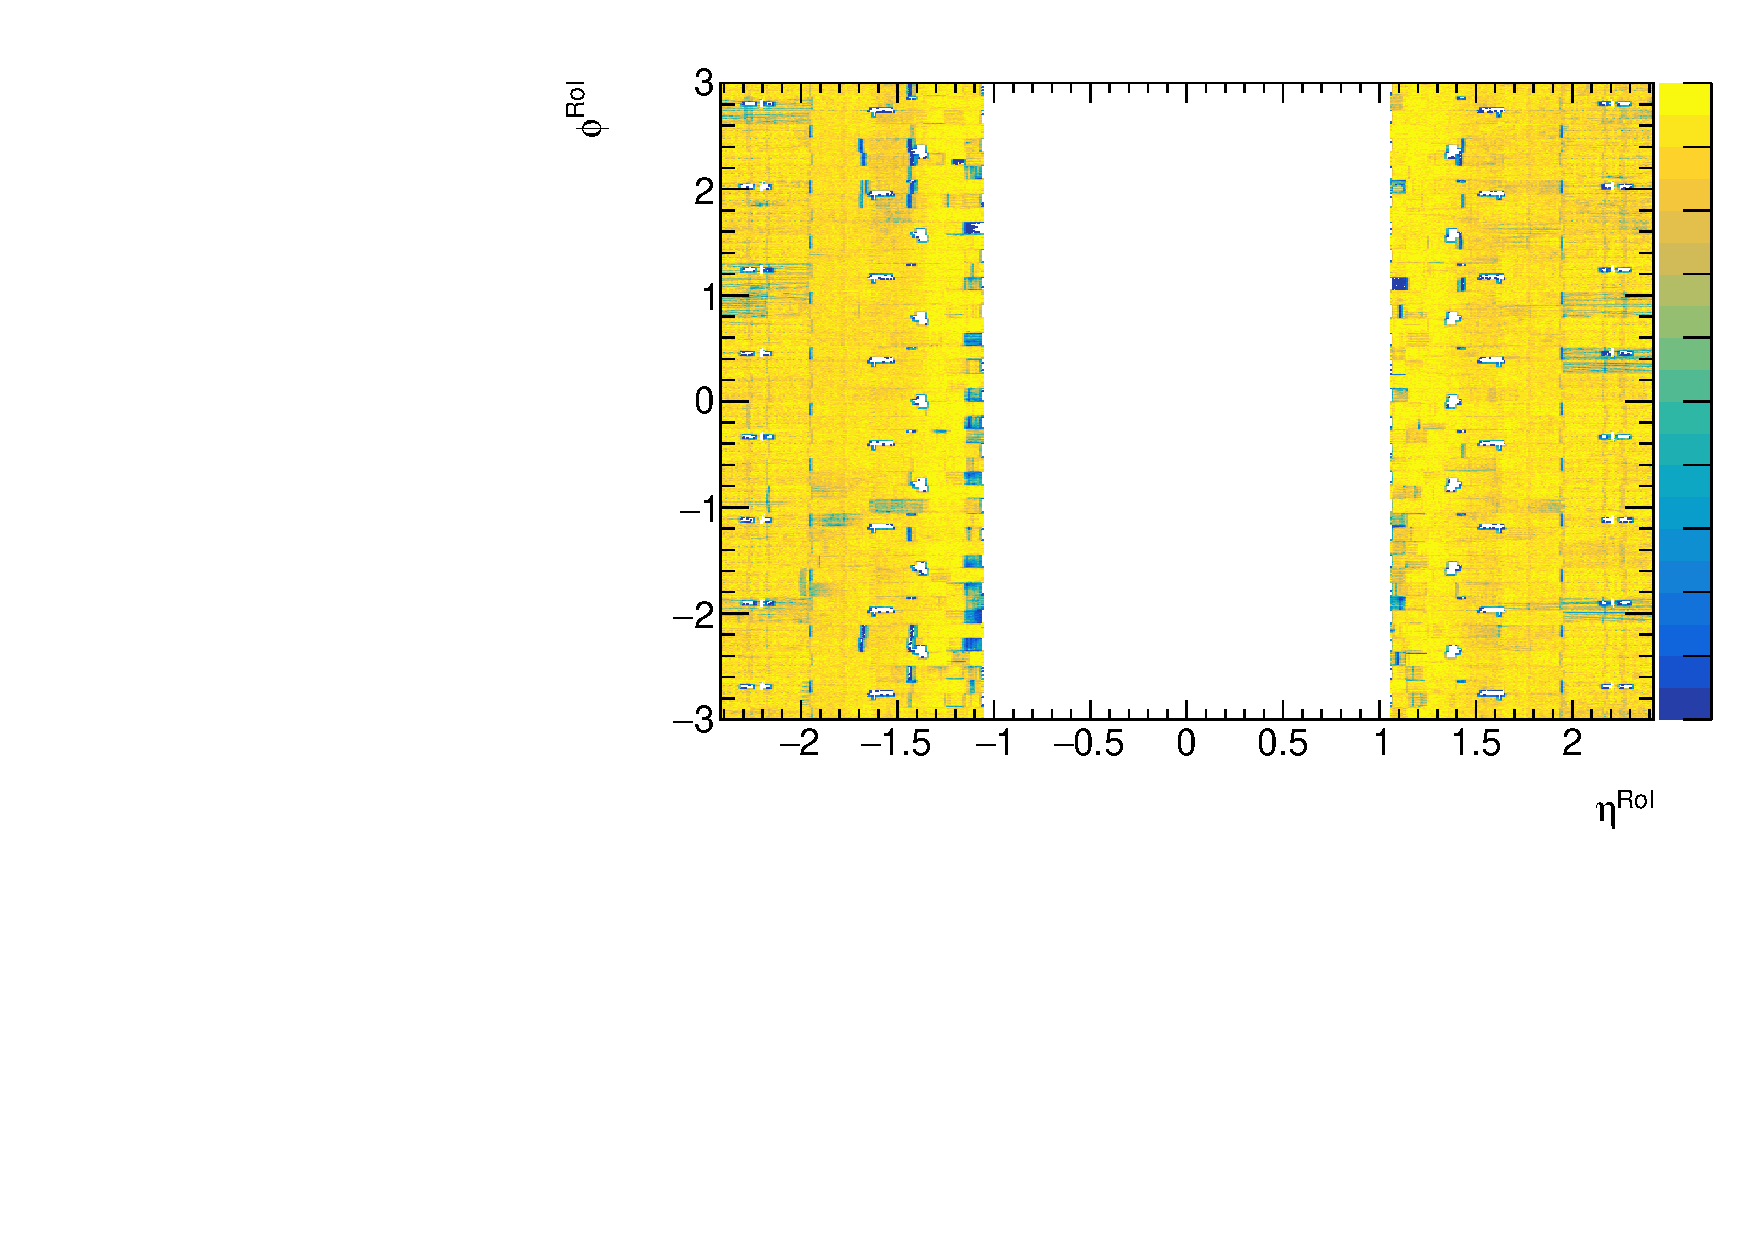
\includegraphics[clip, width=7cm]{fig/5/h2_v0514_Eff.pdf}
%        %\vspace{5pt}
%        \subcaption{}
%        \label{fig:v05EffMU14}
%    \end{minipage}%
%    \end{tabular}
%    \caption{TGCのRoIにおけるトリガー効率。分母を$p_{\rm{T}}$が20~GeV以上のオフライン再構成されたミューオンとし、その中で$p_{\rm{T}}$閾値14~GeVのトリガーを鳴らしたミューオンの割合を表している。(a):$\mathrm{CW_{Data}}$(b):$\mathrm{CW_{2022}}$}
 %   \label{EffMU14}
%\end{figure}



%低い$p_{\rm{T}}$閾値のトリガーに対しての課題があるが、トレーニングデータの低い$p_{\rm{T}}$のミューオン数を増加させることや、適切な重みをつけてトレーニングを行うことで、

%\include{chapter6}
%\include{chapter7}

\chapter{結論と展望}\label{chapter6}



\newpage
\chapter*{謝辞}
\addcontentsline{toc}{chapter}{謝辞}

\newpage
\bibliography{ref.bib}
%\bibliographystyle{unsrturl}
%\bibliographystyle{junsrt}
\bibliographystyle{atlasBibStyleWithTitle.bst}
\newpage

\newpage
\thispagestyle{empty}
%~
%\newpage
    
\end{comment}

\end{document}